\documentclass[12pt,titlepage,dvipdfmx]{jarticle}

%お好みに合わせて変えてください
\usepackage[top=30truemm,bottom=30truemm,left=25truemm,right=25truemm]{geometry}
\usepackage{hyperref}
\usepackage{amsmath,amssymb}
\usepackage[utf8]{inputenc}
\usepackage{physics}
\usepackage{color}
\usepackage{url}
\usepackage{here}
\usepackage{ascmac}
\usepackage[dvipdfmx]{graphicx}
\usepackage{siunitx}
\usepackage{cite}
\usepackage{here}


\hypersetup{
    colorlinks=true,
    linkcolor=blue,
    filecolor=magenta,      
    urlcolor=cyan,
    pdftitle={Sharelatex Example},
    %bookmarks=true,
    pdfpagemode=FullScreen,
}

\title{カゴメ格子上の$J_1 - J_2$古典$XY$反強磁性体の有限温度相図}
\author{埼玉大学大学院理工学研究科 博士前期課程\\物理機能系専攻 物理学コース\\20MP104 柿澤文哉 }

\begin{document}

\maketitle

\newpage

\begin{abstract}
幾何学的フラストレート磁性体における基底状態の巨視的縮退は様々な摂動に対して敏感に破れ、複雑な相構造や豊富な相転移が現れる。
そのため、過去数十年に渡って数多くの研究が行われてきた。
典型的な幾何学的フラストレート磁性体であるカゴメ格子上の最近接古典$XY$反強磁性体もその一つで、基底状態に巨視的な縮退を持つ。
この巨視的縮退は温度によって解消され、系は有限温度でカイラリティ長距離秩序を伴わない八極子準長距離秩序のBKT転移\cite{Berezinskii1972,Kosterlitz1973}を示す\cite{Rzchowski1997}。
また、次近接相互作用は絶対零度において巨視的縮退を解消し、$q=0$秩序や$\sqrt{3}\times\sqrt{3}$秩序といったカイラリティ長距離秩序を伴う磁気秩序が現れる\cite{Harris1992}。
一方で、巨視的縮退に対する次近接相互作用と温度の協奏効果という基本的な物理は未解明であった。
本研究では、次近接相互作用と温度の協奏効果が巨視的縮退に与える影響を数値的に解明するため、ループ更新や非平衡緩和法を用いた大規模古典モンテカルロ計算によってカゴメ格子上の$J_1-J_2$古典$XY$反強磁性体の有限温度相図を作成した。
その結果、$-7\times10^{-2}\le J_2\le-7.5\times10^{-3}$に明確な一次転移を発見した。
また、$J_2=0$における八極子秩序が$q=0$相と$\sqrt{3}\times\sqrt{3}$相との間に中間相を形成していることを確認した。
さらに、一次転移の低温側の臨界終点は常磁性相・$q=0$相・八極子相の相境界に近接している。これは低温での一次転移消失と八極子相の存在の間の関係を示唆している。
   


\end{abstract}

\tableofcontents

\newpage

\newpage 

\section{イントロダクション}
\subsection{相転移現象}
相転移現象(以降、単に相転移)は、何らかのパラメータを連続的に変化させたとき、ある値を境に系の定性的な性質が不連続に変化する現象を指す。
相転移前後の同一の性質を示すパラメータ領域を相という。
それぞれの相は相の秩序構造を反映した物理量である秩序変数によって特徴づけられ、相転移は秩序変数の不連続変化によって記述される。
また、相転移は次数によっても特徴づけられる。$n$次相転移は自由エネルギー$F$の$n$階微分$\pdv*[n]{F}{X}$が転移点$X=X_{\mathrm{c}}$で発散することと定義される。
相転移は自発的対称性の破れの有無で大別される。

後者の代表例が水における固体--液体相転移(固液相転移)と気体--液体相転移(気液相転移)である。
水の場合はパラメータとして圧力$P$と温度$T$を使うことが多く、$P-T$平面($P-T$相図)に固相・液相・気相が存在する。
大気圧下では$0\si{\degreeCelsius}$において固液相転移、$100\si{\degreeCelsius}$において気液相転移を示す。
(摂氏温度における$0\si{\degreeCelsius}$と$100\si{\degreeCelsius}$の定義)。
ここでの秩序変数は密度であり、$0\si{\degreeCelsius}$と$100\si{\degreeCelsius}$で不連続に変化する。
固液相転移と気液相転移はともに一次相転移である。

そして、前者の代表例が磁性体における常磁性--強磁性相転移である。
このような磁性体は高温では熱ゆらぎによって強磁性を示さないが、転移温度($T=T_{\mathrm{c}}$)を境にゼロ磁場下で自発磁化($m=\pm m_{\mathrm{s}})$を示す。
$m=m_{\mathrm{s}}$を与える状態と$m=-m_{\mathrm{s}}$を与える状態は全スピン反転対称性によって結ばれており、同等のエネルギーを持つ。
しかし、常磁性--強磁性転移の際には外的要因なしに(自発的に)$m=\pm m_{\mathrm{s}}$のどちらかが選ばれ実現する。
これが自発的対称性の破れである。秩序変数は自発磁化$m_{\mathrm{s}}$である。
また、多くの場合、自発的対称性の破れを伴う相転移は二次相転移となる。

一方で、磁性体における相転移が必ずしも自発的対称性の破れを伴うわけではない。
むしろ、自発的対称性の破れを伴う相転移が禁制された状況下で、系独自の秩序や相転移を示す点に磁性体研究の面白さがある。
本研究は磁性体における相転移を対象とする。

\subsection{{古典スピン模型}}
一般的に、相転移は巨視的な数の構成要素が相互作用して起きる協働現象である。
したがって、磁性体における相転移を記述するためには、磁性体内部の構成要素と、それらの間の相互作用を記述する微視的模型が必要となる。
古典統計力学の範囲でこの役割を果たすのが(局在)古典スピン模型である。
%磁性は原子・電子が持つスピン自由度がマクロな数存在することによって発現する。
%現代の磁性研究の主流は、ミクロな構成要素であるスピンとスピン間の相互作用から出発し、磁性というマクロな性質を説明することである。
%物質中のスピン間の相互作用を記述するのが(局在)古典スピン模型である。
$N$個のスピン系を仮定すると、最大$N$体の相互作用が考えられるが、二体の交換相互作用のみを考えれば、
強磁性など典型的な磁性現象を説明できる。ハミルトニアンは以下で与えられる。
\begin{align}
   H = \sum_{(ij)} J_{ij} \vec{S}_i\cdot \vec{S}_j.
\end{align}
$\vec{S}_i$は格子点$i$上で定義される単位ベクトルを表し、$J_{ij}$は交換相互作用を表す。
$(ij)$は互いに交換相互作用を及ぼすスピンの組を表す。
理論上、$\vec{S}$の次元に制限はないが、磁性研究では三次元までが対象となることが多く、次元に応じて
\begin{itemize}
   \item $\vec{S}=(0,0,S^z)$の場合、イジング(Ising)スピン
   \item $\vec{S}=(S^x,S^y,0)$の場合、$XY$スピン
   \item $\vec{S}=(S^x,S^y,S^z)$の場合、ハイゼンベルグ(Heisenberg)スピン
\end{itemize}
と呼ばれる。
%スピンがイジング/$XY$/ハイゼンベルグスピンであるとき、古典スピン模型もイジング/$XY$/ハイゼンベルグ模型と呼ばれることがある。

\subsection{古典スピン模型による常磁性--強磁性転移の説明}
磁性体における常磁性--強磁性転移は交換相互作用のみを考慮した古典スピン模型によって説明できる。
説明のために隣り合う格子点(最近接格子点)上のスピン間のみに強磁性的交換相互作用が働くことを仮定する。
\begin{align}
   H_{\mathrm{NN}} = \sum_{\ev{ij}} J_{ij} \vec{S}_i\cdot \vec{S}_j,\ J_{ij}<0\ (\forall{\ev{ij}}).
\end{align}
統計力学によると、絶対零度($T=0$)では内部エネルギー最低の状態(基底状態)が最大のボルツマン重みを持つ。
これは$\vec{S}_i\cdot\vec{S}_j=1\ (\forall{\ev{ij}})$を満たす、すべてのスピンが同方向に揃った強磁性状態である。
一方で、高温極限ではエントロピーが大きい常磁性状態が最大ボルツマン重みを持つ。
よって、高温極限と絶対零度の間で最大ボルツマン重みを持つ状態が常磁性状態から強磁性状態に切り替わり、常磁性--強磁性転移が起こる。
また、$J_{ij}<0$はスピンの方向を揃えることから強磁性的交換相互作用という。

%これはすべてのスピンが同方向に揃った強磁性状態である。
%$\vec{S}_i\cdot\vec{S}_j=1\ (\forall{ij})$を満たす状態が最低エネルギーとなるが、
%これはすべてのスピンが同方向に揃った強磁性状態である。
%一方で、$J_{ij}>0\ (\forall{ij})$のとき、$\vec{S}_i\cdot\vec{S}_j=-1\ (\forall{ij})$の状態が最低エネルギーとなるが、
%これは隣り合うすべてのスピンが互いに逆方向を向いた反強磁性状態である。
%これを以て$J_{ij}<0$を強磁性的、$J_{ij}>0$を反強磁性的(交換相互作用)と呼ぶ。
%
%上の議論から$J_{ij}=0\ (\forall{ij})$を境に系の最低エネルギー状態が強磁性/反強磁性状態から反強磁性/強磁性状態へ定性的に変化する。
%(厳密には$J_{ij}=0$の最低エネルギー状態は任意のスピン配置なので、$J_{ij}=0$は含まない。)
%また、これまでの議論では暗に絶対零度($T=0$)を仮定していたが、高温極限$(J/T<<1)$ではスピンが何ら秩序を示さない常磁性状態が支配的となり、
%系は常磁性を示す。したがって、絶対零度から温度を上昇させていったとき、ある温度を境に系の磁性が(反)強磁性から常磁性へ定性的に変化することが想像される。
%このように何らかのパラメータを連続的に変化させたとき、ある値を境に系の性質が定性的かつ不連続に変化する現象を相転移現象という。

%次節では相転移現象一般について述べた後、特に磁性体に関連する過去の相転移研究の結果を紹介する。

%\newpage

%\subsection{相転移現象}
%相転移現象(以降、単に相転移)は、何らかのパラメータを連続的に変化させたとき、ある値を境に系の性質が定性的かつ不連続に変化する現象を指す。
%より詳細に述べると、相転移前後の同一の性質を示すパラメータ領域を相といい、パラメータ変化に伴い、
%相間を移ることによって、系の性質が定性的かつ不連続に変化する。
%現代の相転移研究では、それぞれの相は相の秩序構造を反映した物理量である秩序変数によって特徴づけられ、相転移は秩序変数の不連続変化によって記述されることが多い。
%また、相転移は次数によっても特徴づけられる。$n$次相転移の定義は自由エネルギー$F$の$n$階微分$\pdv*[n]{F}{X}$が転移点$X=X_{\mathrm{c}}$で発散することである。
%
%
%相転移の最も身近な例として水における相転移が挙げられる。
%水の場合はパラメータとして圧力$P$と温度$T$を使うことが多く、$P-T$平面($P-T$相図)に固相・液相・気相が存在する。
%大気圧下では$0\si{\degreeCelsius}$において固体ー液体相転移、$100\si{\degreeCelsius}$において液体ー気体相転移を示す。
%(摂氏温度における$0\si{\degreeCelsius}$と$100\si{\degreeCelsius}$の定義)。
%ここでの秩序変数は密度であり、$0\si{\degreeCelsius}$と$100\si{\degreeCelsius}$で不連続に変化することが知られている。
%固体ー液体相転移と液体ー気体相転移はともに一次相転移である。
%
%本題である磁性体に関する相転移について説明する。
\subsection{マーミン・ワグナーの定理}
常磁性--強磁性と同様に、離散対称性と連続対称性の自発的破れも古典スピン模型によって説明できる。
まず、離散対称性の場合を議論する。
簡単のため、強磁性的な最近接相互作用のみを考慮した二次元正方格子上のイジング模型を考える。
この模型は厳密解が存在し、有限温度$T=T_{\mathrm{c}}$で二次相転移を示すことが分かっている。
$T<T_{\mathrm{c}}$では強磁性状態が支配的となり、$T=0$では全てのスピンが$S_i^z=1$あるいは$S_i^z=-1$に揃っている。
これら二つの状態はエネルギー的に縮退しているため、エネルギーの損得はないが、必ずどちらかが選ばれる。
よって、全スピンに対する反転対称性(離散対称性)が自発的に破れている。
同じように、$XY$/ハイゼンベルグ模型などの連続対称性を示す模型において、基底状態から唯一つ状態が選ばれることを連続対称性の自発的破れという。

磁性体における相転移に関する最も重要な定理の一つにマーミン・ワグナーの定理\cite{Mermin1966}がある。
この定理は以下を主張している。
\begin{center}
   二次元以下の格子では、有限温度で連続対称性の自発的破れを伴う相転移は存在しない。
\end{center}

%対称性の自発的破れについては前述した。
%ここでは古典スピン模型を用いて、繰り返しを恐れず、離散対称性と連続対称性の自発的破れについて議論する。
%まず、離散対称性の場合を議論する。
%簡単のため、最近接相互作用のみの二次元正方格子上のイジング模型を考える。強磁性的な相互作用を仮定する。
%この模型は厳密解が存在し、有限温度$T=T_{\mathrm{c}}$で二次相転移を示すことが分かっている。
%$T<T_{\mathrm{c}}$では強磁性状態が支配的となり、$T=0$では全てのスピンが$S_i^z=1$あるいは$S_i^z=-1$に揃っている。
%これら二つの状態はエネルギー的に縮退しているため、エネルギーの損得はないが、必ずどちらかが選ばれる。
%この状況を全スピンに対する反転対称性が自発的に破れている、という。
%同じように、$XY$/ハイゼンベルグ模型などの連続対称性を示す模型において基底状態から唯一つ状態が選ばれることを連続対称性の自発的破れという。
%マーミン・ワグナーの定理は二次元以下の格子系において、そのような連続対称性の破れを伴う有限温度での相転移が存在しないことを主張している。

%%では、マーミン・ワグナーの定理があるため、二次元以下の格子上の$XY$/ハイゼンベルグ模型について、もはや
%%興味深い問題は残っていないのだろうか。
%%答えは否で、本研究で扱う幾何学的フラストレート磁性体という複数の相互作用が拮抗するスピン模型は
%%\begin{itemize}
%%   \item BKT転移[発見者3名の名前を忘れた。後で調べておく。]
%%   \item (幾何学的)フラストレート磁性体
%%   \item カイラリティなどの、離散対称性を示す新規秩序
%%\end{itemize}
%%が挙げられる。本節ではBKTについてのみ説明し、残りの二つは次節以降で説明する。
%
%%\newpage
%
\subsection{幾何学的フラストレート磁性体}
相互作用によるエネルギー利得を局所的に最大化する条件が系全体で同時に満足できない状況を、フラストレーションがあるという。
一般的に、磁性体はフラストレーションの有無で大別される。
フラストレーションがない磁性体の代表例が二次元正方格子上の反強磁性イジング模型である。
最近接相互作用のみを考慮すると、ハミルトニアンは
\begin{align}
   H = J\sum_{\ev{ij}}\vec{S}_i\cdot\vec{S}_j,\ J>0.
\end{align}
この模型の基底状態は隣り合うスピンが互いに逆方向を向いた状態である。
このとき、すべての局所的な相互作用利得が最大の$-J$になるため、フラストレーションはない。

フラストレーションがある磁性体の代表例が三角形上の反強磁性イジング模型である。
先程と同じハミルトニアンを考える。
基底状態の例として、まず上サイトにアップスピン、左下サイトにダウンスピンを配置する。
このとき、右下サイトにアップスピンとダウンスピンを配置したどちらの状態も基底状態となる。
しかし、アップスピンの場合は上サイトと、ダウンスピンの場合ば左下サイトとの相互作用利得を損する。
したがって、どのような基底状態にも相互作用利得が$J$となる組が存在するため、フラストレーションがある。
特に、フラストレーションが格子の幾何学的特徴に起因するとき、その磁性体を幾何学的フラストレート磁性体という。
三角形上の反強磁性イジング模型は最も簡単な幾何学的フラストレート磁性体である。

また、強磁性的な相互作用を考慮した模型ではフラストレーションは生じない。
よって、以降は特に注意しない限り、反強磁性的な最近接相互作用を考慮する。
%上サイトのスピンとの相互作用利得を最大化するためにはダウンスピンを配置すればよいが、このとき左下サイトのスピンとは最大化できない。
%アップスピンを配置した場合でも事情は同様である。
%したがって、三つのスピンが互いに逆向きであるという局所的エネルギー利得最大化条件を系全体で同時に満足できない。
%この状況を指して、系にフラストレーションがあるといい、さらにフラストレーションが三角形という幾何学的特徴に由来するため、この系には幾何学的フラストレーションがある、という。
%特に、格子の幾何学的特徴によるフラストレーションを幾何学的フラストレーション、磁性体を幾何学的フラストレート磁性体という。
%最も簡単な幾何学的フラストレート磁性体は三角形上の反強磁性イジング模型である。この模型を用いて(幾何学的)フラストレーションを説明する。

\begin{figure}[H]
 \begin{minipage}{0.5\hsize}
  \begin{center}
   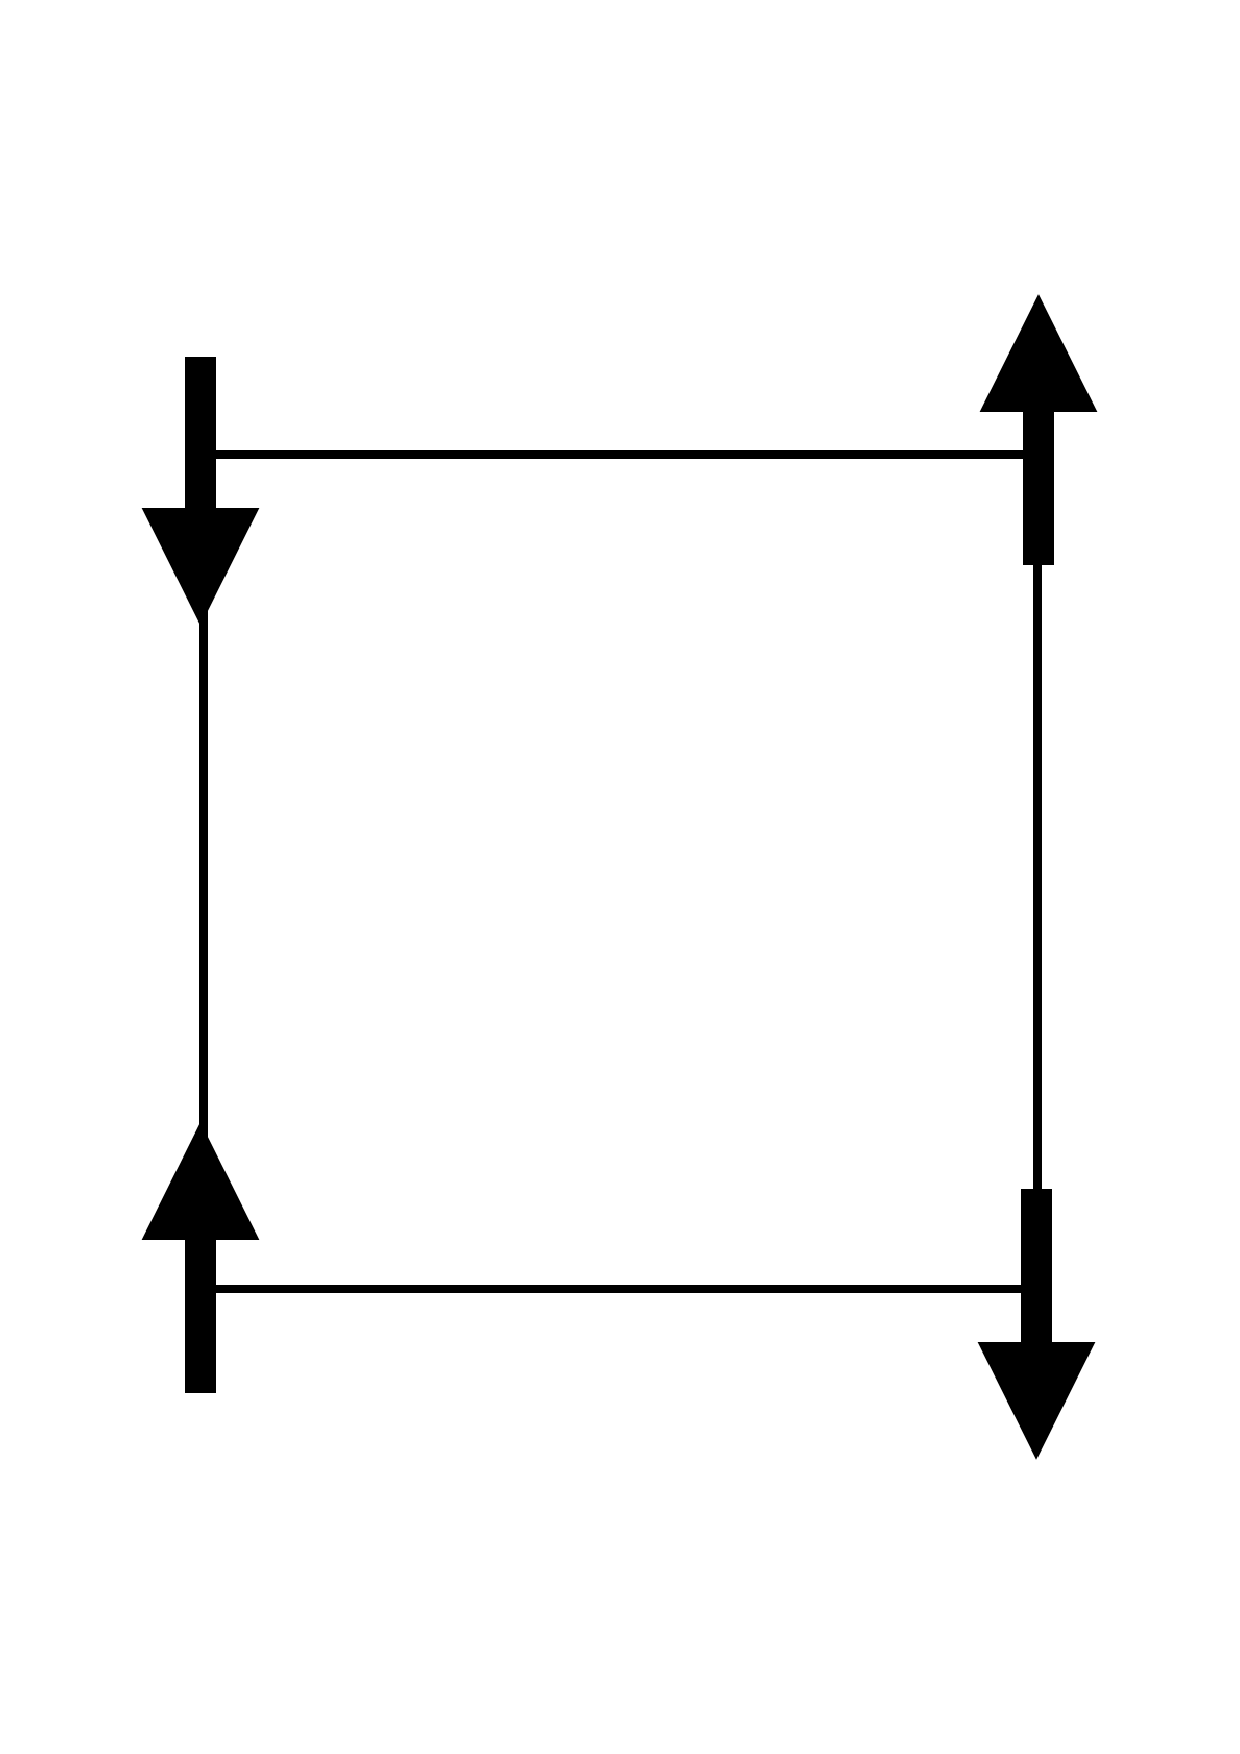
\includegraphics[width=43mm]{figure/square_ising_afm.pdf}
  \end{center}
  \caption{正方格子上の反強磁性イジング模型}
  %\label{fig:one}
 \end{minipage}
 \begin{minipage}{0.5\hsize}
  \begin{center}
   \includegraphics[width=55mm]{figure/triangle_ising_afm.pdf}
  \end{center}
  \caption{三角形上の反強磁性イジング模型}
  %\label{fig:two}
 \end{minipage}
\end{figure}
   
%まず、相互作用を得するよう、上サイトにアップスピン、左下サイトにダウンスピンを配置する。右下のサイトにスピンを配置する。
%上サイトのスピンとの相互作用利得を最大化するためにはダウンスピンを配置すればよいが、このとき左下サイトのスピンとは最大化できない。
%アップスピンを配置した場合でも事情は同様である。
%したがって、三つのスピンが互いに逆向きであるという局所的エネルギー利得最大化条件を系全体で同時に満足できない。
%この状況を指して、系にフラストレーションがあるといい、さらにフラストレーションが三角形という幾何学的特徴に由来するため、この系には幾何学的フラストレーションがある、という。

いくつかの幾何学的フラストレート磁性体は、マクロ系において基底状態の縮退数が格子点数に対して指数関数的に増加するという顕著な性質を示す。
これを基底状態の巨視的縮退という。
特にフラストレーションが強いカゴメ格子では、$XY$スピンなどの連続スピン模型においても巨視的縮退が残る。
本研究ではカゴメ格子上の$XY$反強磁性体を扱う。

%巨視的縮退数は格子やスピンの種類で変化する。
%本研究の主題であるカゴメ格子上の古典反強磁性$XY$模型は次節以降に譲り、本章では三角格子とカゴメ格子上の古典反強磁性イジング模型について過去の結果を整理する。
%\subsection{基底状態の巨視的縮退}
%フラストレート系の最大の特徴は、三角形を結合したマクロな格子系において、基底状態の縮退数がスピン数に対して指数関数的に増加することである。
%このような縮退を巨視的縮退という。
%本節では、まず非自明な縮退について述べ、二つの三角形を結合したフラストレート系において三角形模型よりも基底状態の縮退数が増加することを見て、
%最後にマクロなフラストレート系の代表例である三角格子とカゴメ格子の巨視的縮退について過去の結果を紹介する。
%
%非自明な縮退を考える前に、まず自明な縮退として、正方格子上の反強磁性イジング模型における基底状態の縮退を考える。
%この模型の基底状態はアップスピンとダウンスピンが交互に並ぶ状態であるが、この状態は全てのスピンが反転した状態とだけ縮退している。
%この縮退はハミルトニアンの対称性から明らかであるため、自明な縮退である。
%非自明な縮退として、やはり三角形上の反強磁性イジング模型における基底状態の縮退を考える。
%この模型の基底状態は異なる三つの状態にそれぞれ自明な二重縮退があり、六重縮退している。
%三つの状態は全スピン反転によって互いに行き来できないため、ハミルトニアンの対称性に由来しない非自明な縮退となっている。
%
%自明な縮退における縮退数は高々ハミルトニアンの対称性程度$\mathcal{O}(1)$であるため、マクロな格子系における巨視的縮退をもたらすのは非自明な縮退である。
%ここから、辺共有結合三角形上の反強磁性イジング模型(辺共有模型、図2)と頂点共有結合三角形上の反強磁性イジング模型(頂点共有模型、図3)を用いて、
%非自明な縮退がある場合、どちらの模型の基底状態においても縮退数が三角形模型より増加すること、辺共有模型よりも頂点共有模型の方が縮退数が多いことを示す。
%
%\begin{figure}[H]
% \begin{minipage}{0.5\hsize}
%  \begin{center}
%   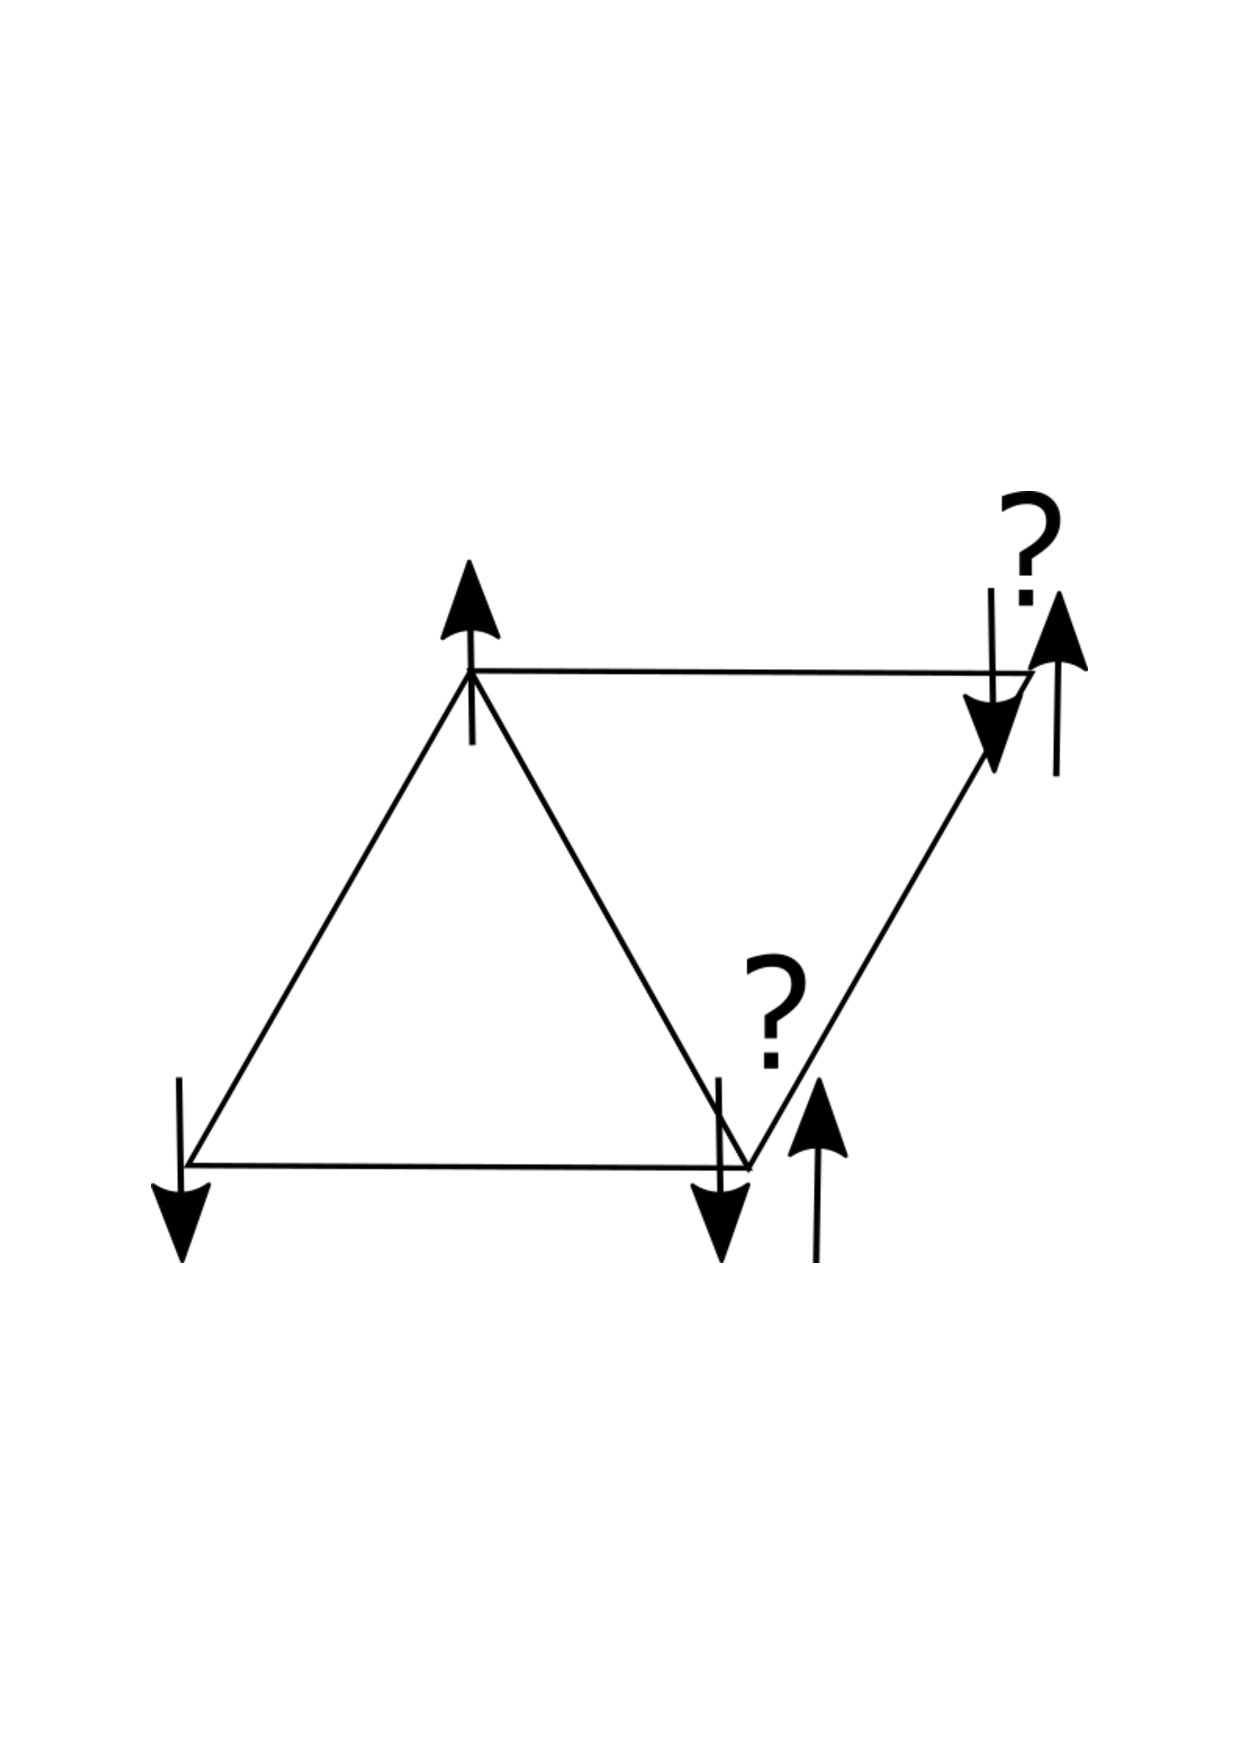
\includegraphics[width=50mm]{figure/edge_shared_triangle.pdf}
%  \end{center}
%  \caption{辺共有三角形上のイジング模型}
%  \label{fig:one}
% \end{minipage}
% \begin{minipage}{0.5\hsize}
%  \begin{center}
%   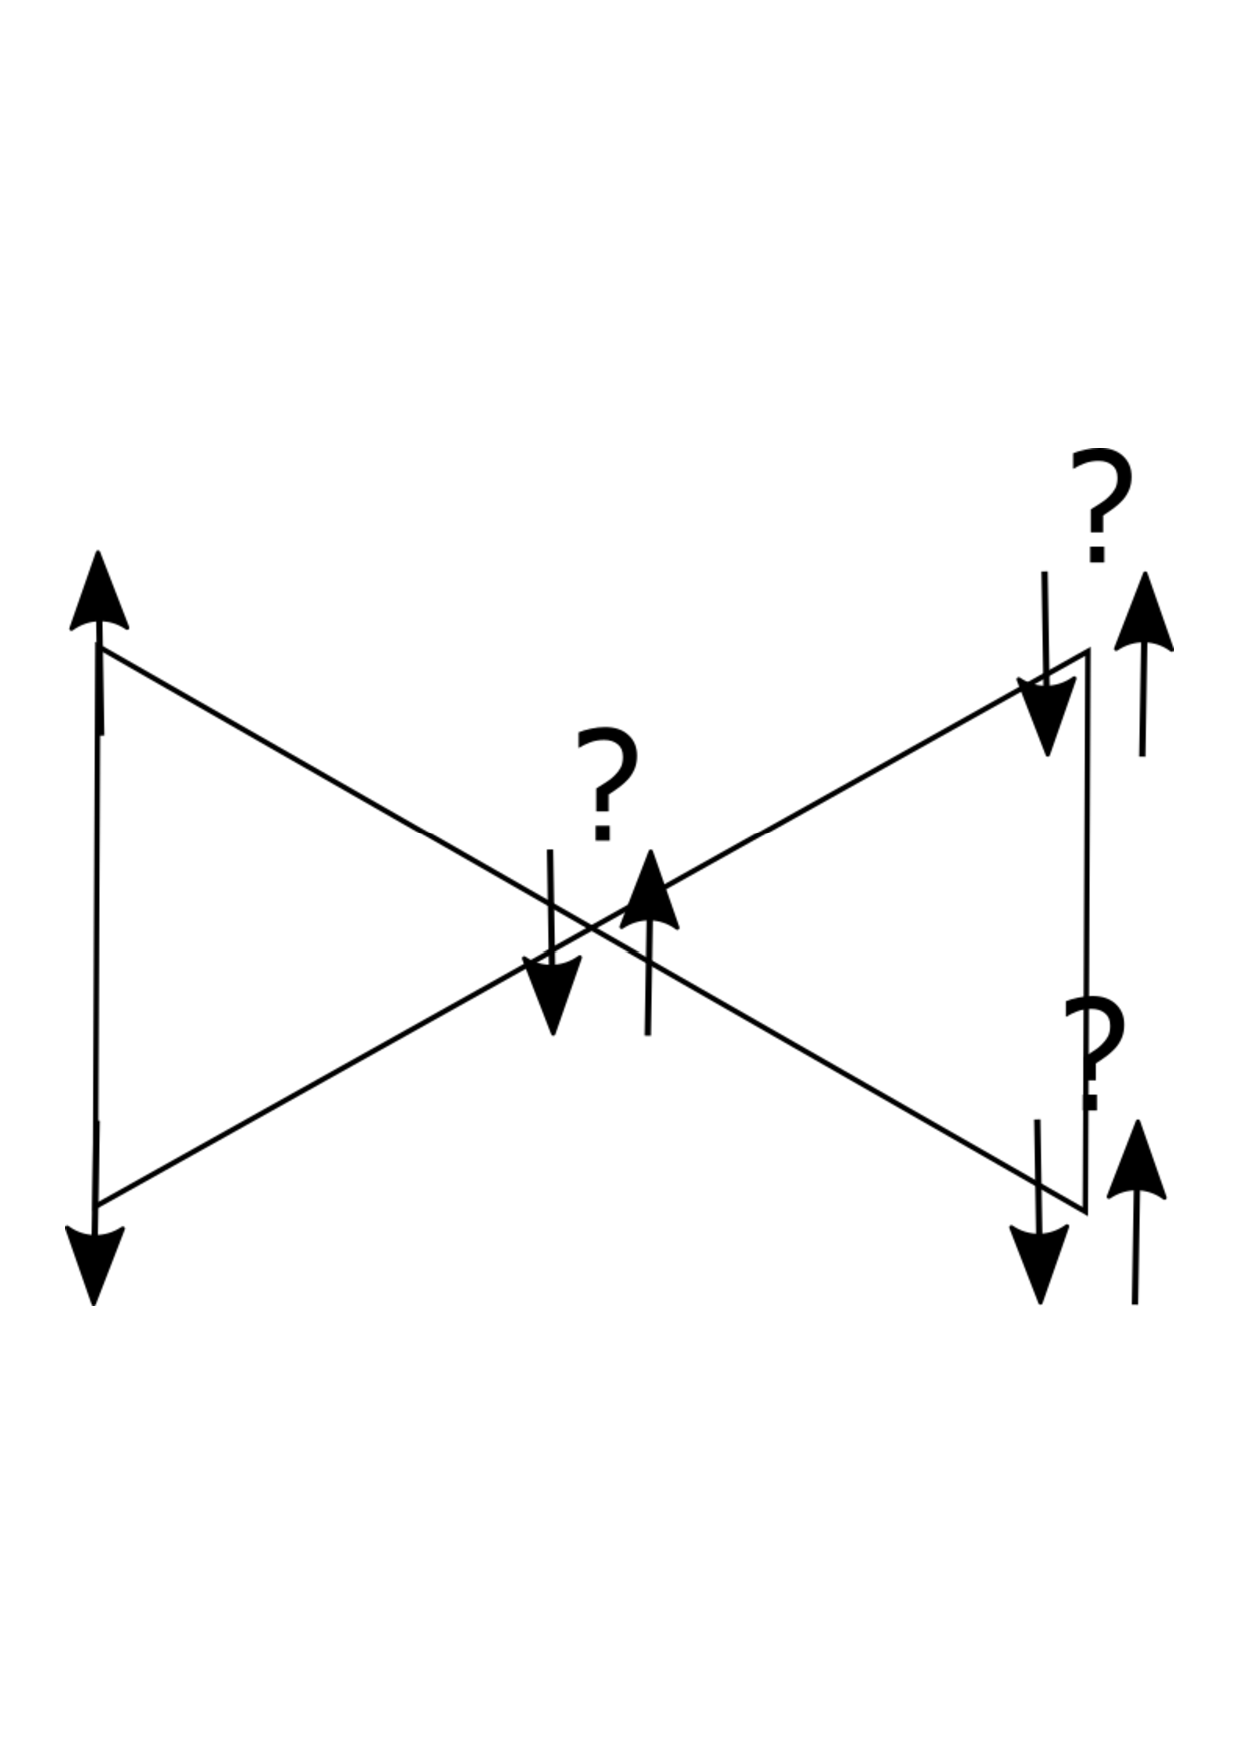
\includegraphics[width=55mm]{figure/top_shared_triangle.pdf}
%  \end{center}
%  \caption{頂点共有三角形上のイジング模型}
%  \label{fig:two}
% \end{minipage}
%\end{figure}
%
%まず辺共有模型の基底状態を考える。図2の上向き三角形だけを見れば三角形模型と同じであるから、図1と同じようにスピンを配置すればよい。
%右上のサイトにはどちらのスピンを配置すればよいか。右下サイトにアップスピンが入った場合はダウンスピンを配置すればよい。
%問題はダウンスピンが入った場合で、このときは右上のサイトがフラストレートしてしまう。したがって辺共有模型は三角形模型より基底状態における縮退数が多い。
%次に頂点共有模型を考える。先と同様に図3の左の三角形に図1と同じようにスピンを配置しよう。残った右の三角形の上下サイトにスピンを配置する。
%共有サイトとエネルギー利得を最大化するように上サイトにスピンを配置すると、下サイトは三角形模型と同じ理由でフラストレートする。
%はじめに下サイトにスピンを配置しても事情は同じである。したがって頂点共有模型も三角形模型より基底状態における縮退数が多い。
%また、辺共有模型と頂点共有模型を比べると頂点共有模型の方が縮退数が多い。
%これは共有しているサイトが少なく、フラストレートしているサイトのうち一つのスピンを決めても、これによってスピンが決まるサイトが少ないためである。
%
%最後に、マクロなフラストレート系の代表例である三角格子上の反強磁性イジング模型(三角格子模型、図xx)と
%カゴメ格子上の反強磁性イジング模型(カゴメ模型、図xx)における基底状態の巨視的縮退について過去の結果を紹介する。
%
%ここまで見てきたように、マクロなフラストレート系において、基底状態が巨視的に縮退し、絶対零度まで相転移が抑制される場合がある。
%これを踏まえて、初期のフラストレート系研究では縮退数や低温下のスピン相関の空間構造などが研究されてきたが、
%近年になって、巨視的縮退が外部磁場や異方性などの摂動によって敏感に解消され、有限温度において相転移を示すことが分かってきた。
%
%本研究では摂動としてより一般的かつ現実的な次近接相互作用$J_2$を導入し、有限温度での振る舞いを調べた。研究に用いた模型、先行研究、動機の詳細は次章で述べる。
%
\newpage

%\section{先行研究}
\section{カゴメ格子上の$J_1-J_2$古典反強磁性$XY$模型}
\subsection{$J_2=0$}
ハミルトニアンは最近接相互作用のみの場合、
\begin{align}
   H_{\mathrm{NN}} = J_1\sum_{\ev{ij}}\vec{S}_i\cdot\vec{S}_j .
\end{align}
$\ev{ij}$は最近接格子点の組を表す。反強磁性相互作用$J_1=1$のみを考える。
\subsubsection{$T=0$}
ハミルトニアンを副格子ごとの和で書き直す。
\begin{align}
   H_{\mathrm{NN}} = \sum_{\mathrm{sublattice}} (\vec{S}_1+\vec{S}_2+\vec{S}_3)^2 + \mathrm{const.}
\end{align}
添字は副格子内の格子点を表す。よって、各副格子内で以下の条件を満たす全ての状態が基底状態となる。
\begin{align}
   \vec{S}_1+\vec{S}_2+\vec{S}_3 = 0
\end{align}
この条件を満たす副格子内のスピン配置として、以下の$120^\circ$構造がある。
\begin{figure}[H]
   \centering
   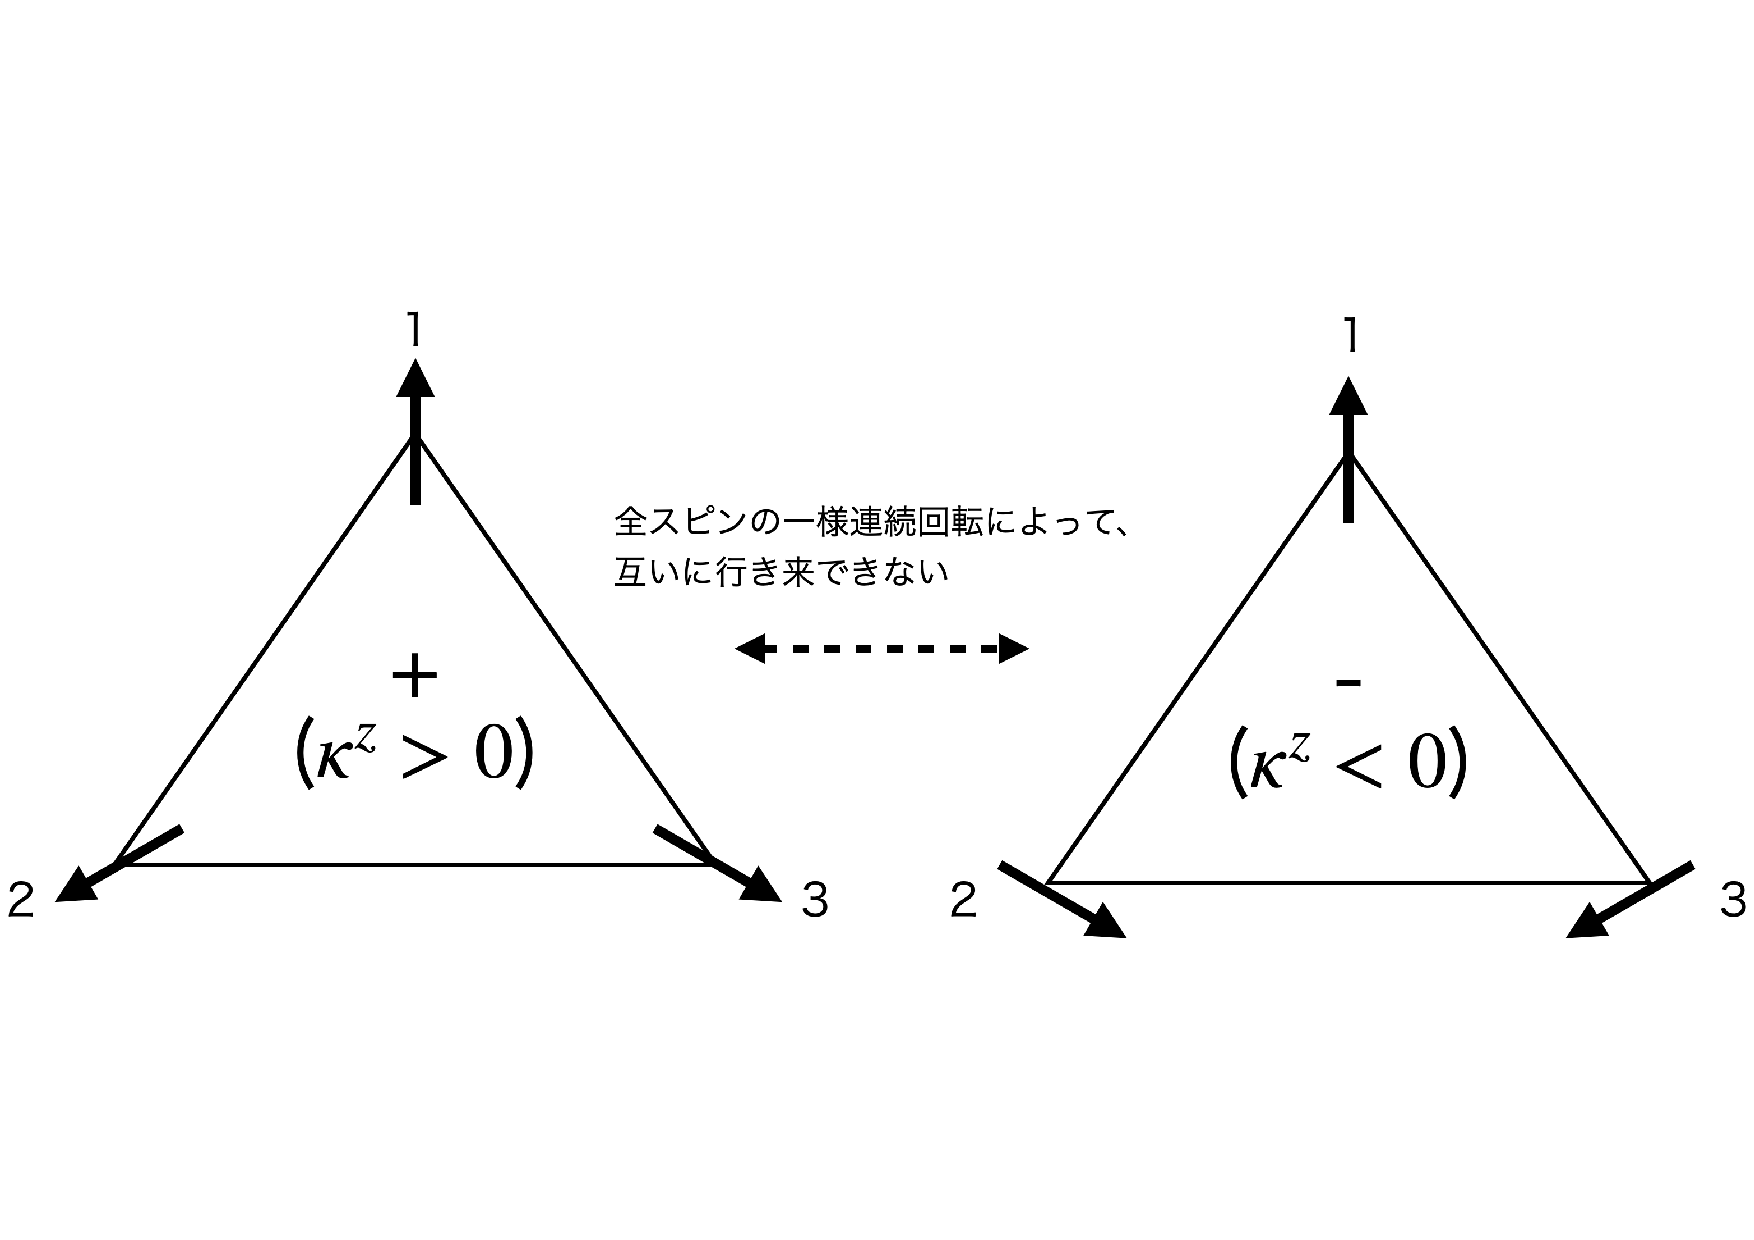
\includegraphics[width=10cm]{figure/120degs_structures.pdf}
   \caption{カイラリティ符号が異なる二つの$120^\circ$構造}
\end{figure}

$120^\circ$構造はカイラリティ自由度によって特徴づけれられる。
カイラリティは副格子ごとに
\begin{align}
   \kappa \equiv \frac{2}{3\sqrt{3}}(\vec S_1 \times \vec S_2 + \vec S_2 \times \vec S_3 + \vec S_3 \times \vec S_1)
\end{align}
で定義される。
全系の基底状態は各副格子に$120^\circ$構造を配置して得られる。
基底状態の縮退数$N_{\mathrm{GS}}$は三色問題の解であり、格子点数を$N$として
\begin{align}
   N_{\mathrm{GS}} = 1.13471^{N}
\end{align}
となる\cite{Baxter2003}。よって、本模型は$J_2=0$において基底状態の巨視的縮退を示す。

%[田畑氏のレビューによると、Baxterの数値は間違っていて、後年修正されたという。]
%・三角格子状の反強磁性$XY$模型の基底状態は巨視的縮退を示さない。


\subsubsection{$T\neq0$}
%幾何学的フラストレート磁性体における基底状態の巨視的縮退は有限温度での長距離相転移を抑制する。
一般的に、基底状態の巨視的縮退は有限温度での長距離相転移を抑制する。
一方で、この巨視的縮退は様々な摂動に対して敏感に破れ、その際、系は独自の秩序を示す。
この現象はゆらぎによる秩序(order by disorder)と呼ばれる。
代表的なゆらぎである熱ゆらぎは八極子秩序をもたらす\cite{Huse1992}。
八極子秩序の特徴は各副格子が$120^\circ$構造を持ち、かつカイラリティの長距離秩序を示さない点である。
さらに、八極子秩序は有限温度でBerezinskii-Kosterlitz-Thouless(BKT)転移\cite{Berezinskii1972,Kosterlitz1973}を示す。
BKT転移は、スピン相関関数が距離に対して指数関数的に減衰する長距離相転移と異なり、冪的に減衰する。
そのため、BKT転移を示す秩序は準長距離秩序となる。
八極子準長距離秩序のBKT転移温度は$T = 0.070\sim0.076$と報告されている\cite{Rzchowski1997}。
\begin{figure}[H]
   \centering
   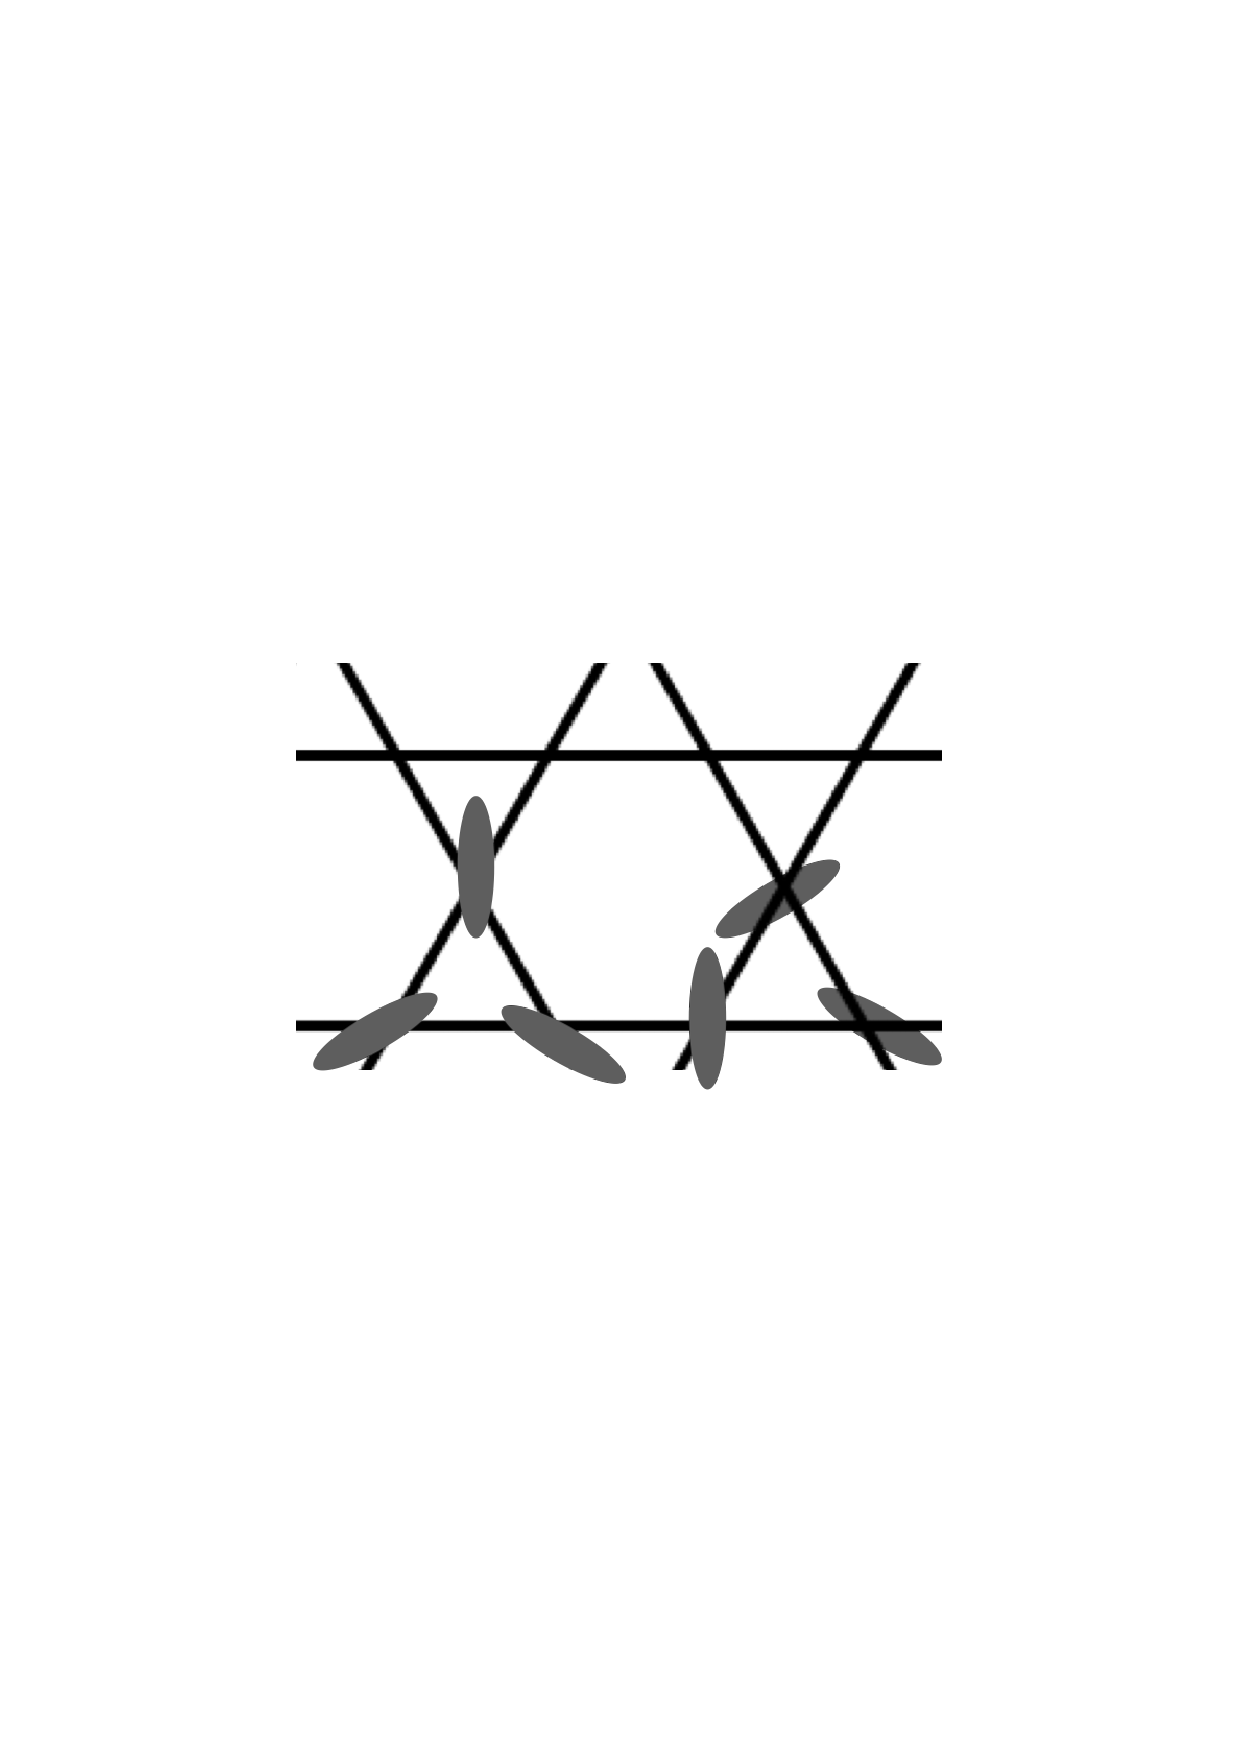
\includegraphics[scale=0.5]{figure/schematic_octupole_order.pdf}
   \caption{八極子秩序のスピン配置の概念図}
\end{figure}

%\begin{itemize}
%   \item 有限温度での八極子準長距離秩序のBKT転移が存在する
%   \item 八極子相は磁気的準長距離秩序が存在しつつ、カイラリティ長距離秩序が存在しない相である。
%   \item_
%\end{itemize}


\subsection{$J_2\neq0$}
ハミルトニアンは$J_2\neq0$の場合、
\begin{align}
   H = J_1\sum_{\ev{ij}}\vec{S}_i\cdot\vec{S}_j + J_2\sum_{\ev{\ev{ij}}}\vec{S}_i\cdot\vec{S}_j .
\end{align}
$\ev{\ev{ij}}$は次近接格子点の組を表す。
\subsubsection{$T=0$}
次近接相互作用$J_2$によって$J_2=0$における基底状態の巨視的縮退が解消される。
$J_2/J_1<0$の場合は$q=0$状態、$J_2/J_1>0$の場合は$\sqrt{3}\times\sqrt{3}$状態が基底状態となる\cite{Harris1992}。
%網掛け部分が磁気的秩序のユニットセルである。また、区別のため$120^\circ$構造の三種類のスピンを三色に塗り分けた。
これら二つの状態はそれぞれ磁気秩序とカイラリティ秩序を示す。
各図の網掛け部分が磁気秩序のユニットセルに対応する。
さらに、$q=0$状態は強磁性的な、$\sqrt{3}\times\sqrt{3}$は反強磁性的なカイラリティ$\kappa^z$の符号秩序を示す。
このように連続スピン系でありながら、基底状態が離散対称性の秩序を示す点が$J_2\neq0$の特徴である。
%カイラリティ秩序は符号秩序であるため、あたかも各副格子の中心にイジングスピンが存在し、それらが(反)強磁性秩序を示している、と見ることもできる。

%\begin{itemize}
%   \item 次近接相互作用$J_2$によって$J_2=0$における基底状態の巨視的縮退が解消される。
%   \item $J_2/J_1<0$の場合は$q=0$状態、$J_2/J_1>0$の場合は$\sqrt{3}\times\sqrt{3}$状態が基底状態となる。
%   \item 二つの状態はそれぞれ磁気秩序とカイラリティ秩序を示す。
%   \item 磁気秩序のユニットセルは各図の網掛け部分に対応する。
%   \item 副格子ごとのカイラリティ符号
%   \item $q=0$では
%   \item $\sqrt{3}\times\sqrt{3}$では
%   \item よって
%   
%\end{itemize}

\begin{figure}[H]
   \begin{minipage}{0.5\hsize}
    \begin{center}
     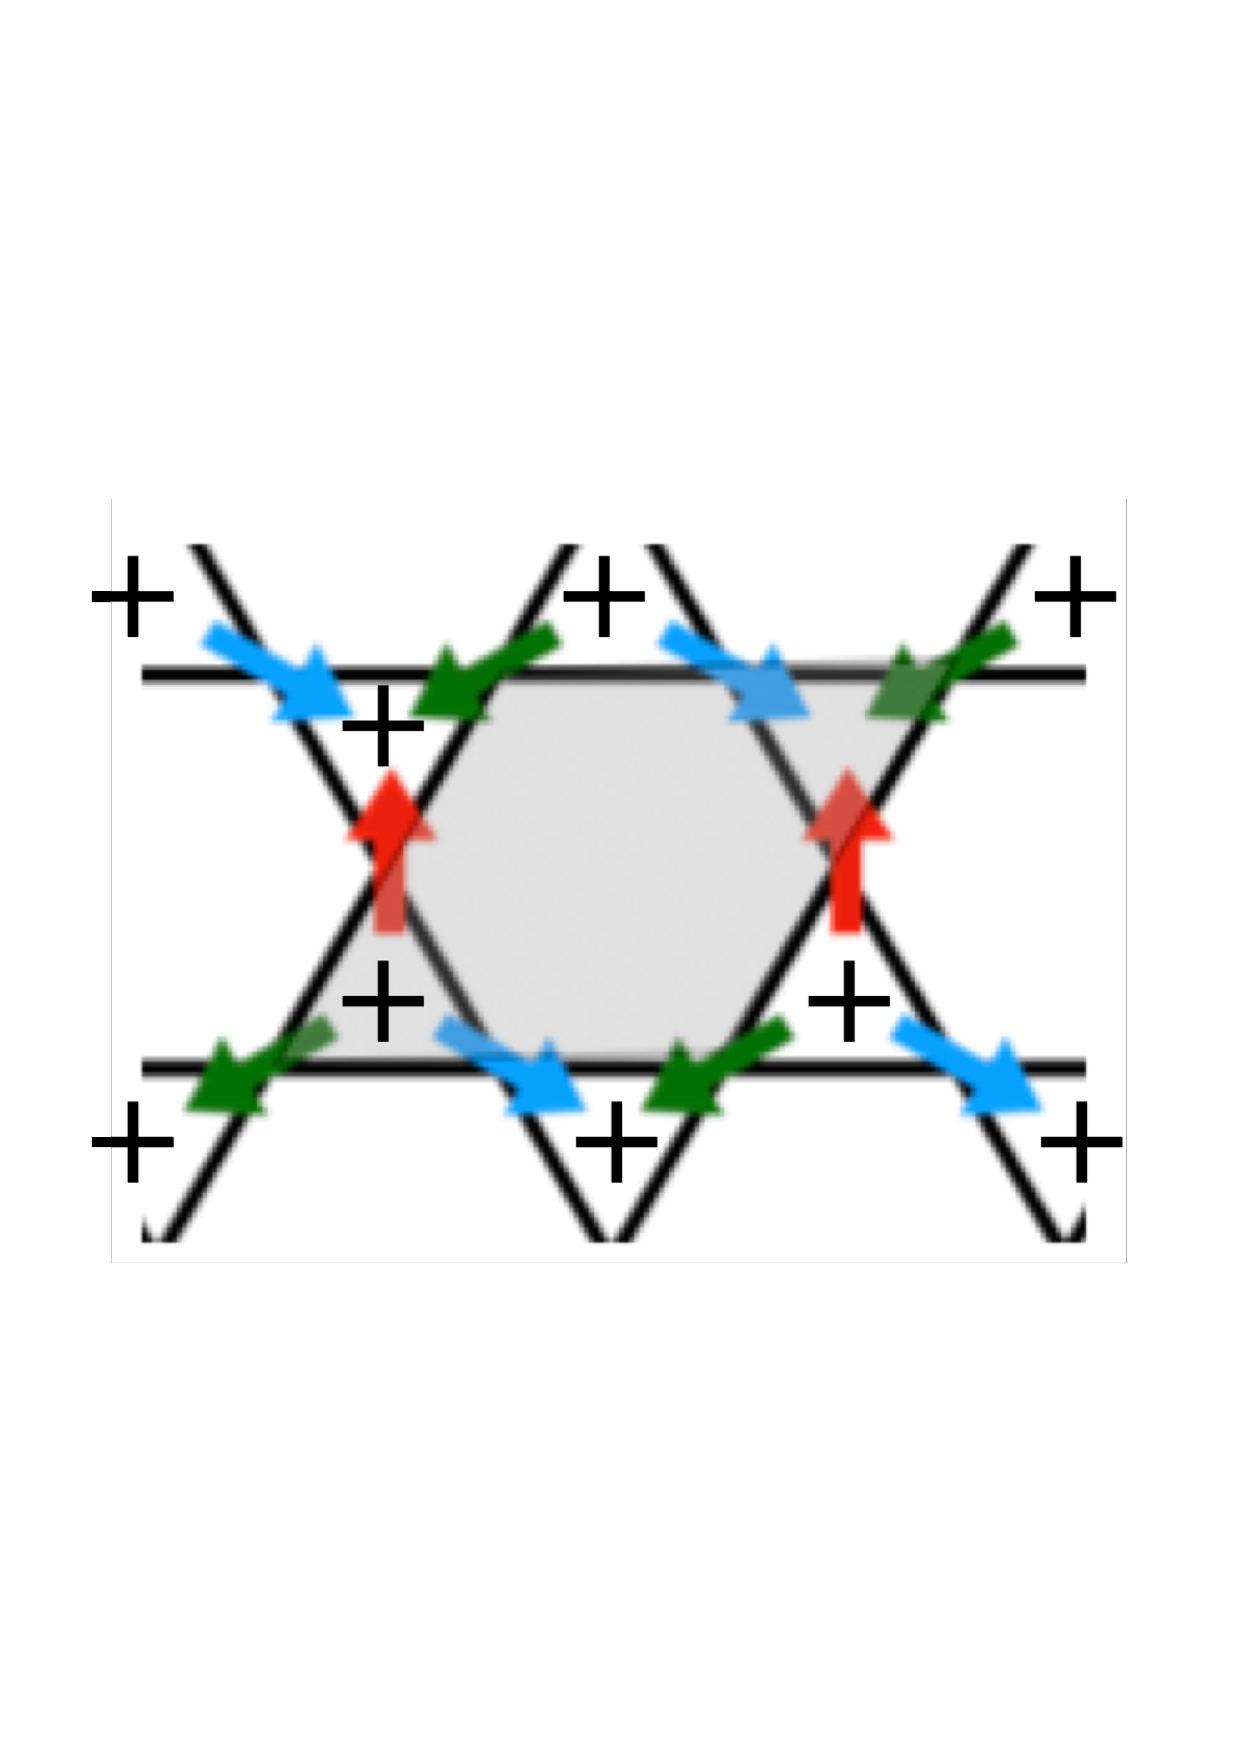
\includegraphics[width=6cm]{figure/q0.pdf}
    \end{center}
    \caption{$q=0$構造}
    %\label{fig:one}
   \end{minipage}
   \begin{minipage}{0.5\hsize}
    \begin{center}
     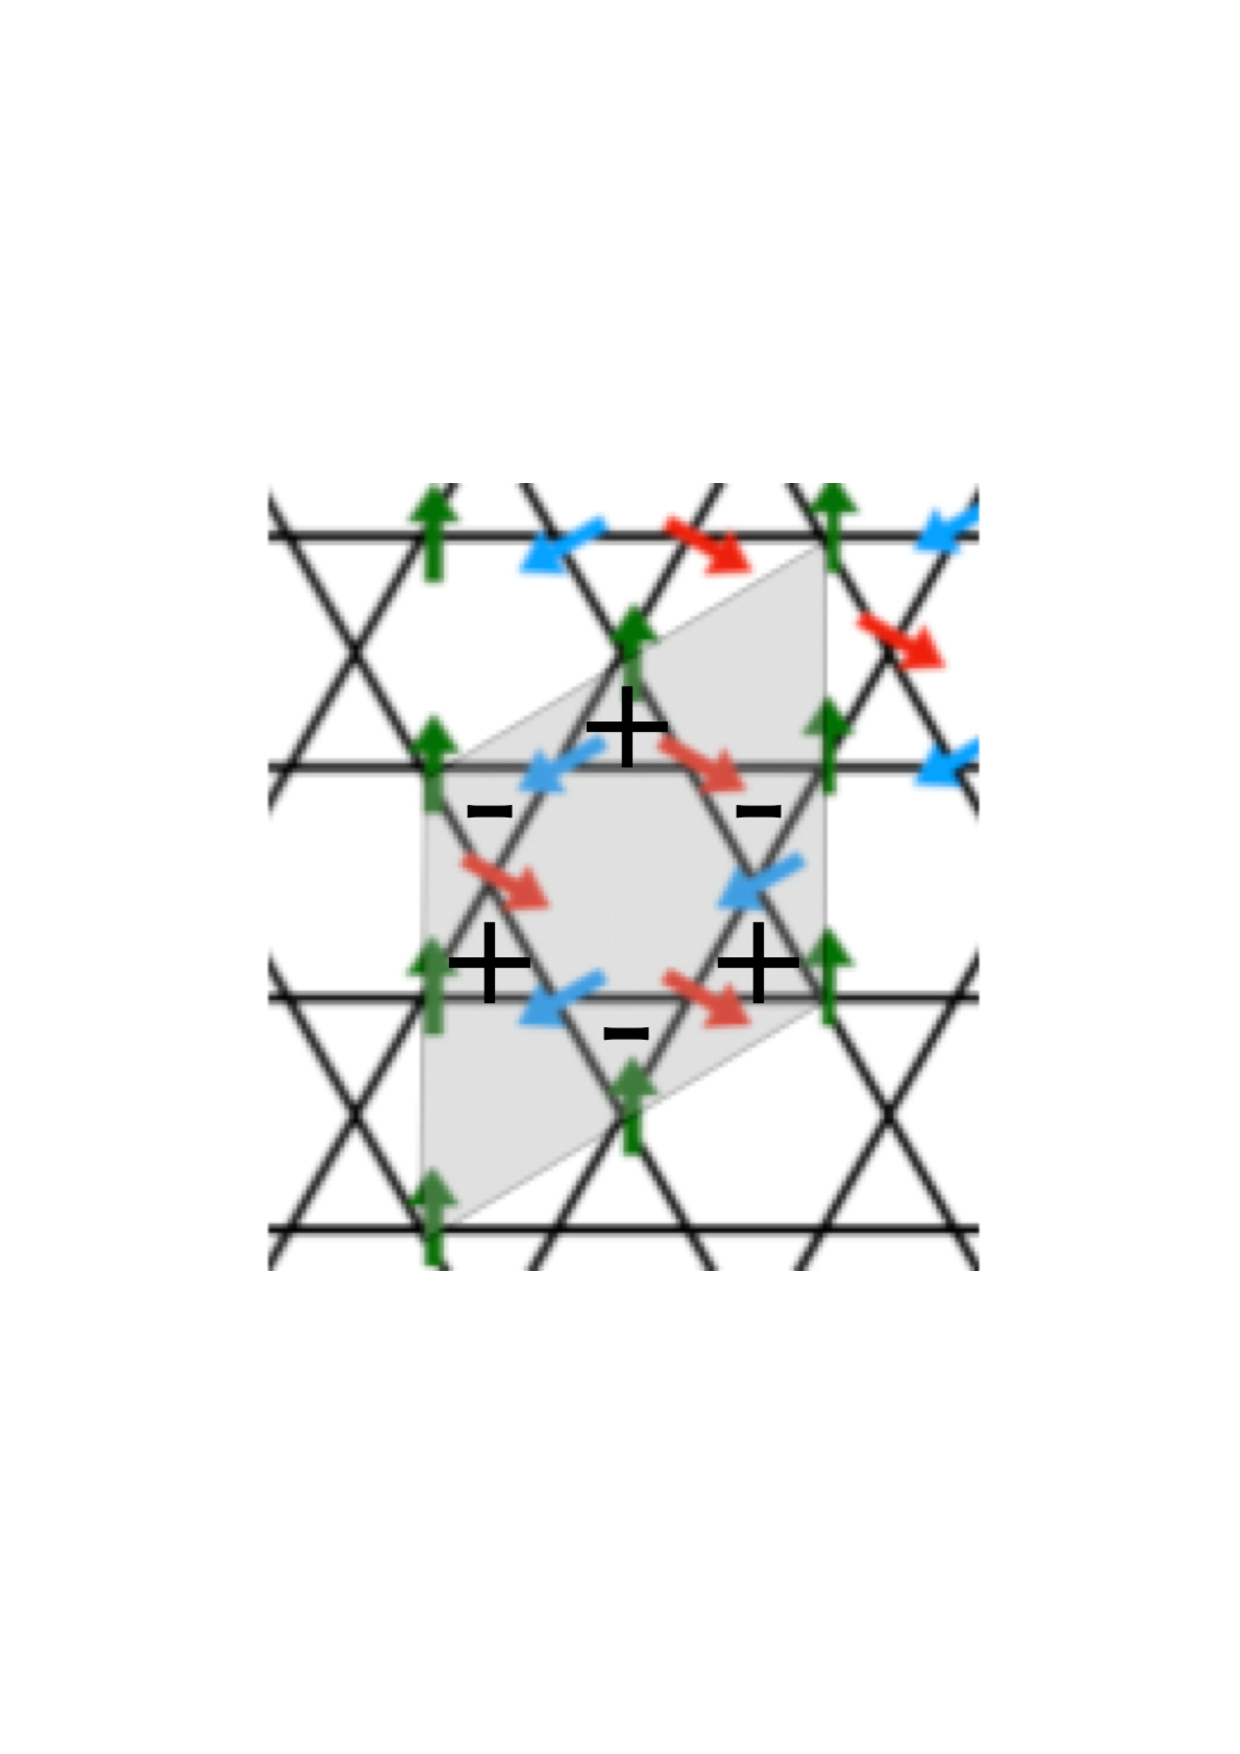
\includegraphics[width=5cm]{figure/sqrt3.pdf}
    \end{center}
    \caption{$\sqrt{3}\times\sqrt{3}$構造}
    %\label{fig:two}
   \end{minipage}
\end{figure}

%\begin{itemize}
%   \item 基底状態の巨視的縮退が$J_2$によって解消され、$\sqrt{3}\times\sqrt{3}(J_2/J_1>0)$構造、$q=0(J2/J1<0)$構造が基底状態となる。
%   \item $\sqrt{3}\times\sqrt{3}$構造は反強磁性的カイラリティ、$q=0(J_2/J_1<0)$構造は強磁性的カイラリティを示す。
%\end{itemize}


\subsubsection{$T≠0$}
現象論的な先行研究によって得られた概念的$J_2-T$相図を示す\cite{Korshunov2002}。実線が(反)強磁性的カイラリティ転移温度、破線が八極子秩序のBKT転移温度を表す。
この相図は$q=0$(強磁性的カイラリティ)相、$\sqrt{3}\times\sqrt{3}$(反強磁性カイラリティ)相、八極子相、常磁性相の四相からなる。
まず、$T=0$における$q=0$と$\sqrt{3}\times\sqrt{3}$の長距離秩序が有限温度では準長距離秩序に変化し、BKT転移を示す。
(反)強磁性カイラリティ長距離秩序もそれぞれ対応する磁気秩序とほぼ同時に転移するが、$J_2/J_1$が大きい領域では転移温度が分離している。
次に、$J_2=0$における八極子秩序が$-10^{-3}\le J_2/J_1\le 10^{-4}$という非常に狭い領域に残り、$q=0$相と$\sqrt{3}\times\sqrt{3}$相との間に中間相を形成している。
また、八極子相の転移温度は$J_2/J_1$に依存せず一定である。
最後に、相図の原点近傍で$\sqrt{3}\times\sqrt{3}$相が一度$J_2/J_1<0$に張り出し、低温で再び$J_2/J_1=0$線にマージしている。
すなわち、本模型は原点近傍において低温から$q=0$相--八極子相--$\sqrt{3}\times\sqrt{3}相$--八極子相--常磁性相という複雑な相構造を持つ。
\begin{figure}[H]
   \centering
   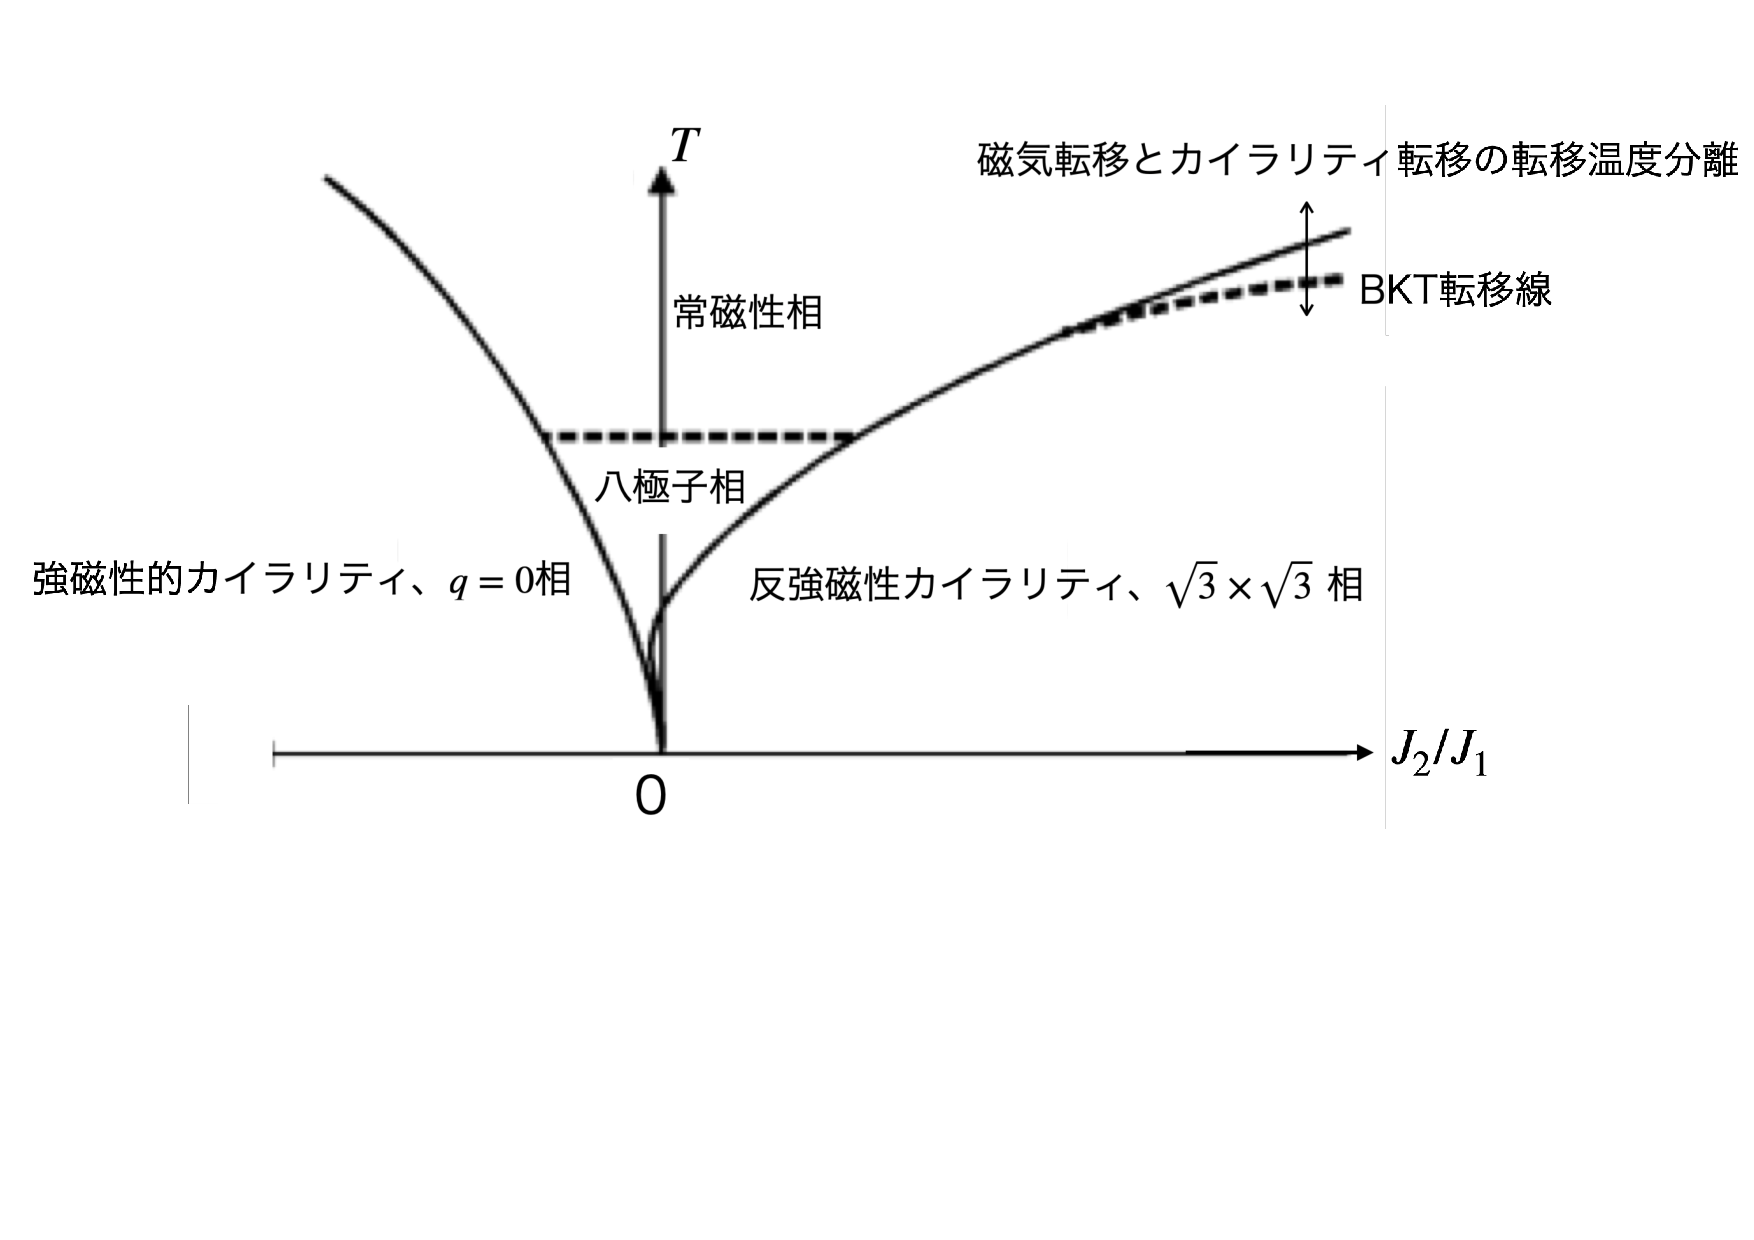
\includegraphics[scale=0.5]{figure/schematic_phase_diagram.pdf}
   \caption{現象論的$J_2-T$相図}
\end{figure}

%\begin{itemize}
%   \item S.E.Korshunovによる現象論によって得られた概念的な$J_2-T$相図を示す。
%   \item 磁気的準長距離秩序($\sqrt{3}\times\sqrt{3}$秩序と$q=0$秩序)は有限温度でBKT転移を示す。
%   \item カイラリティ長距離秩序も磁気的準長距離秩序と同時に転移する。
%   \item $J_2=0$での八極子転移が$J_2\neq0$にも残り、$\sqrt{3}\times\sqrt{3}$相と$q=0$相との中間相となる。
%   \item 八極子相の転移温度は$J_2$に依存せず一定である。
%   \item 相図の原点近傍に$\sqrt{3}\times\sqrt{3}$相が$J_2/J_1<0$側に張り出す構造がある。
%\end{itemize}

\newpage

\section{本研究の動機・目的}
本研究の目的はカゴメ格子上の最近接古典反強磁性XY模型の基底状態の巨視的縮退に対する温度と次近接相互作用の協奏効果を数値的・定量的に解明することである。
これまで述べたように、温度単体・次近接相互作用単体の効果は盛んに研究され、八極子秩序のBKT転移温度など定量的な理解が進んでいる。
一方で、温度と次近接相互作用の協奏効果については、定性的な$J_2-T$相図が提案されたものの、定量的な理解には至っていない。
そこで、本研究では平衡法と非平衡緩和法を組み合わせた大規模な古典モンテカルロ計算を行い、数値的な$J_2-T$相図を作成する。
また、作成した$J_2-T$相図を通して、温度と次近接相互作用の協奏効果を数値的・定量的に解明する。
%先行研究の疑問点を列挙していくと
%\begin{itemize}
%   \item 八極子相が非常に狭い領域($-10^{-3}\le J_2/J_1\le 10^{-4}$)に存在するのは確かか。また、BKT転移温度は$J_2/J_1$に依存せず一定であるのは確かか。
%   \item $J_2/J_1<0$において、$q=0$秩序のBKT転移と強磁性的カイラリティ転移の転移温度は分離しないか。
%   \item 強磁性的カイラリティ転移と反強磁性カイラリティ転移では、転移の次数などは同じか。
%   \item 原点近傍において低温から$q=0$相--八極子相--$\sqrt{3}\times\sqrt{3}相$--八極子相--常磁性相という複雑な相構造を持つのは確かか。
%\end{itemize}
%上記の点を明らかにするため、ループアップデートや非平衡緩和法を利用した大規模な古典モンテカルロ計算を行い、数値的な$J_2-T$相図を作成した。
%
%先行研究を踏まえ、本研究で取り組むべき問題を再定義する。
%その前に、先行研究で分かった点と分からなかった点をそれぞれ整理しておこう。
%
%分かった点。$J2_T$相図を見れば分かることは書かない。
%\begin{itemize}
%   \item $J_2=0$の基底状態は巨視的縮退を示す。
%   \item 警告。書き方に迷うので後回しにする。忘れるなかれ。
%   \item 八極子-常磁性転移のBKT温度$T_{\mathrm{BKT}}$は$J_2$によらず一定。
%\end{itemize}
%
%分からなかった点
%\begin{itemize}
%   \item 転移温度$T_c$の数値
%   \item 相転移の特徴
%   \item $J_2<0(\abs{J_2}\ll1)$のでっぱり。
%   \item 相転移の機構
%\end{itemize}



\newpage

%\section{計算手法}
\section{計算手法}
数値計算にはモンテカルロ法を用いた。モンテカルロ法は乱数を用いた数値計算手法の総称である。
以下の事情から、本研究では平衡法と非平衡緩和法の二つを用いた。
一般的に、平衡熱力学は、十分時間が経過しこれ以上変化しない状態(熱平衡状態)と熱平衡状態間の遷移を扱う。
また、系の詳細によらない普遍的な現象を扱うため、系の大きさを無限大にする理想化を行う。
すなわち、平衡熱力学は時間とシステムサイズの両方を無限大化した系に対して厳密な理論となる。
一方で、計算資源と計算能力の制限から、現実の計算機ではこのような理想化した系をそのまま扱うことはできない。
また、適当な有限化を行って尚、時間とシステムサイズを同時に大きく取る計算は難しい。
そこで、小さな系を長時間計算する平衡法と、大きな系を短時間計算する非平衡緩和法を相補的に組み合わせ、
理想化された系の熱力学的性質を明らかにする。

続く二節で、平衡法と非平衡緩和法について、それぞれ計算する物理量と具体的な手続きを説明する。

%\section{平衡法}
\subsection{平衡法}
%\subsection{計算する物理量}
\subsubsection{計算する物理量}

平衡法では物理量$Q$の熱力学平均
\begin{align}
   \ev{Q} \equiv \frac{\sum_{S\in\Omega}e^{-\beta H(S)}Q(S)}{\sum_{S\in\Omega}e^{-\beta H(S)}}
\end{align}
を計算できる。ここで、$\Omega$は状態空間、$S$は状態、$H$は系のハミルトニアン、$\beta=1/k_{\mathrm{B}}T$は逆温度である。
以降、$k_{\mathrm{B}}=1$とする。本研究で計算する物理量とそれぞれの定義を以下に列挙する。(順不同)

比熱
\begin{align}
   C \equiv \frac{\ev{E^2}-\ev{E}^2}{N_{\mathrm{site}}T^2}.
\end{align}
$N_{\mathrm{site}}$は格子点の総数を表す。

磁気秩序変数
\begin{eqnarray}
   m^2_{\mathrm{\sqrt3\times\sqrt3}} &=& 
   \frac{1}{3N^2_{\mathrm{triangle}}}\sum_{l}\left[\sum_{i} \vec S_l^i \exp\left( \frac{2\pi\mathrm{i}}{3}(x_l^i+y_l^i)\right)\right]^2,\\
   m^2_{q=0}                         &=& 
   \frac{1}{3N^2_{\mathrm{triangle}}}\sum_{l}\left(\sum_{i} \vec S_l^i \right)^2.
\end{eqnarray}
添字$l$は副格子内の格子点番号を表す。

八極子秩序変数
\begin{align}
   m^2_{\mathrm{octupole}} \equiv 
\frac{1}{N_{\mathrm{site}}^2}\left[ \left(\sum_i \cos 3\theta_i \right)^2+\left(\sum_i\sin 3\theta_i\right)^2\right].
\end{align}
$\theta_i$は$i$番目のスピンの$x$軸から測った角度を表す。

(反)強磁性的カイラリティ秩序変数
\begin{eqnarray}
   \kappa_{\mathrm{AFM}}^2 &=& 
   \left[ \frac{1}{N_{\Delta}}\sum_{\mathrm{all}\Delta}\kappa{\Delta} - \frac{1}{N_{\nabla}}\sum_{\mathrm{all}\nabla}\kappa_{\nabla}\right]^2,\\
   \kappa_{\mathrm{FM}}^2  &=& 
   \left[ \frac{1}{N_{\Delta}}\sum_{\mathrm{all}\Delta}\kappa{\Delta} + \frac{1}{N_{\nabla}}\sum_{\mathrm{all}\nabla}\kappa_{\nabla}\right]^2.
\end{eqnarray}
$\kappa_{\Delta,\nabla}$は前述したカイラリティで、計算する副格子(上向三角形$\Delta$と下向三角形$\nabla$)を明記した量である。
すなわち
\begin{align}
   \kappa_{\Delta,\nabla} = \frac{2}{3\sqrt{3}}(\vec S_1 \times \vec S_2 + \vec S_2 \times \vec S_3 + \vec S_3 \times \vec S_1)_{\Delta,\nabla}.
\end{align}
$N_{\Delta},N_{\nabla}$はそれぞれ上向三角形と下向三角形の数を表す($N_{\mathrm{triangle}}=N_{\Delta}+N_{\nabla}$)。

%\subsection{シングルスピンフッリプアップデート}
\subsubsection{シングルスピンフッリプアップデート}
本研究で使用したシングルスピンフリップアップデートを以下にまとめた。

\begin{itembox}[1]{シングルスピンフリップアップデート}
   \begin{enumerate}
       \item 適当な初期状態$\vec{C}_0=(\vec{S}_1,\vec{S}_2,\cdots,\vec{S}_{N_{\mathrm{spin}}})$を用意する。
       \item $\vec{C}_0$のエネルギー$E$を計算する。
       \item $\vec{S}_1$を選ぶ。
       \item $\vec{S}_1$と相互作用するスピンから有効磁場$\vec{h}_{\mathrm{eff}} = \sum _{(1,j)}J_{1j}\vec{S}_j$を計算する。
       \item 新しいベクトル$\vec{S}'_1$を提案する。(一様ランダムフリップ\cite{Liu1988}、ガウシアンムーブ\cite{Evans2014})
       \item 提案前後のエネルギー差$\Delta E = (\vec{S'}_1 - \vec{S}_1) \cdot \vec{h}_{\mathrm{eff}}$を計算する。
       \item 乱数$r(0\le r<1)$を発生させ、$r < P (= \exp(-\beta \Delta E))$であればベクトルを更新する。$r\ge P$であれば元のベクトルに「更新」する。
       \item 更新前後のエネルギー差$\Delta E$を$E$に加える。
       \item $\vec{h}_{\mathrm{eff}}$まわりに$\vec{S}_1$を$\pi$だけ回転させる。(オーバーリラクゼーション\cite{Creutz1987})
       \item 次のスピンに移り、$4\sim9$を繰り返す。
   \end{enumerate}
\end{itembox}


\newpage

%\subsection{レプリカ交換法}
\subsubsection{レプリカ交換法}
%一般に、フラストレート磁性体は低温で複雑なエネルギーランドスケープを持つ。
%一般に、状態が局所的なエネルギー極小地点にトラップされた場合、シングルスピンフリップアップデートのみでは効率的な状態遷移が難しくなる。
一般に、フラストレート磁性体は低温で高温よりも複雑なエネルギー構造を持つ。
また、シングルスピンフリップアップデートのみではエネルギー的なローカルミニマムから効率的に脱出できない。
%したがって、本研究では低温計算において、この問題が顕著になる。
そこで、温度のみが異なる複数の系(レプリカ)を用意し、適宜温度を交換することによって、ローカルミニマムへのトラップを回避する。
この手法をレプリカ交換法\cite{Hukushima2013}という。
本研究で使用したアルゴリズムを以下にまとめた。
\begin{itembox}[2]{レプリカ交換法}
\begin{enumerate}
    \item $\vec{T}=[T_1,T_2,\cdots,T_n]$を用意し,それぞれのレプリカの初期状態を適当に決める。
    %\item 全てのレプリカに対してシングルスピンフリップアップデートを一斉かつ適当な回数行う。
    \item $\vec{T}$の一つ目に対応するレプリカを選ぶ。
    \item 現在のレプリカと右隣のレプリカの状態から$\Delta = (1/T_1 - 1/T_{2})\left(\mathcal{H}(S) - \mathcal{H}(S')\right)$を計算する。
    \item 乱数$r(0\le r<1)$を発生させ、$r<\exp(-\Delta)$であればレプリカを交換する。
    \item 右隣のレプリカに移り4に戻る。右隣にレプリカがない場合6へ進む。
    \item 2に戻る。
\end{enumerate}
\end{itembox}

%\subsection{ループアップデート}
\subsubsection{ループアップデート}
ループアップデートは非局所更新アルゴリズムの一つで、低温で各副格子が$120^\circ$構造をとることと、$120^\circ$構造のうち二種類のスピンを交換してもエネルギー損得がないことを利用する\cite{Schnabel2012}。
下にループアップデートの概念図を示す。三色のシンボルは$120^\circ$構造の三種類のスピンを、赤線は二種類のスピンを結ぶループを表している。
ループ上の緑スピンと青スピンを交換しても、各副格子が$120^\circ$構造をとっている状況は変わらないため、エネルギーが変化しない。
これを利用すればループ上のスピンを同時に更新することができ、局所更新が凍結する低温でも、縮退した状態間を効率的に遷移させることができる。

\begin{figure}[H]
   \centering
   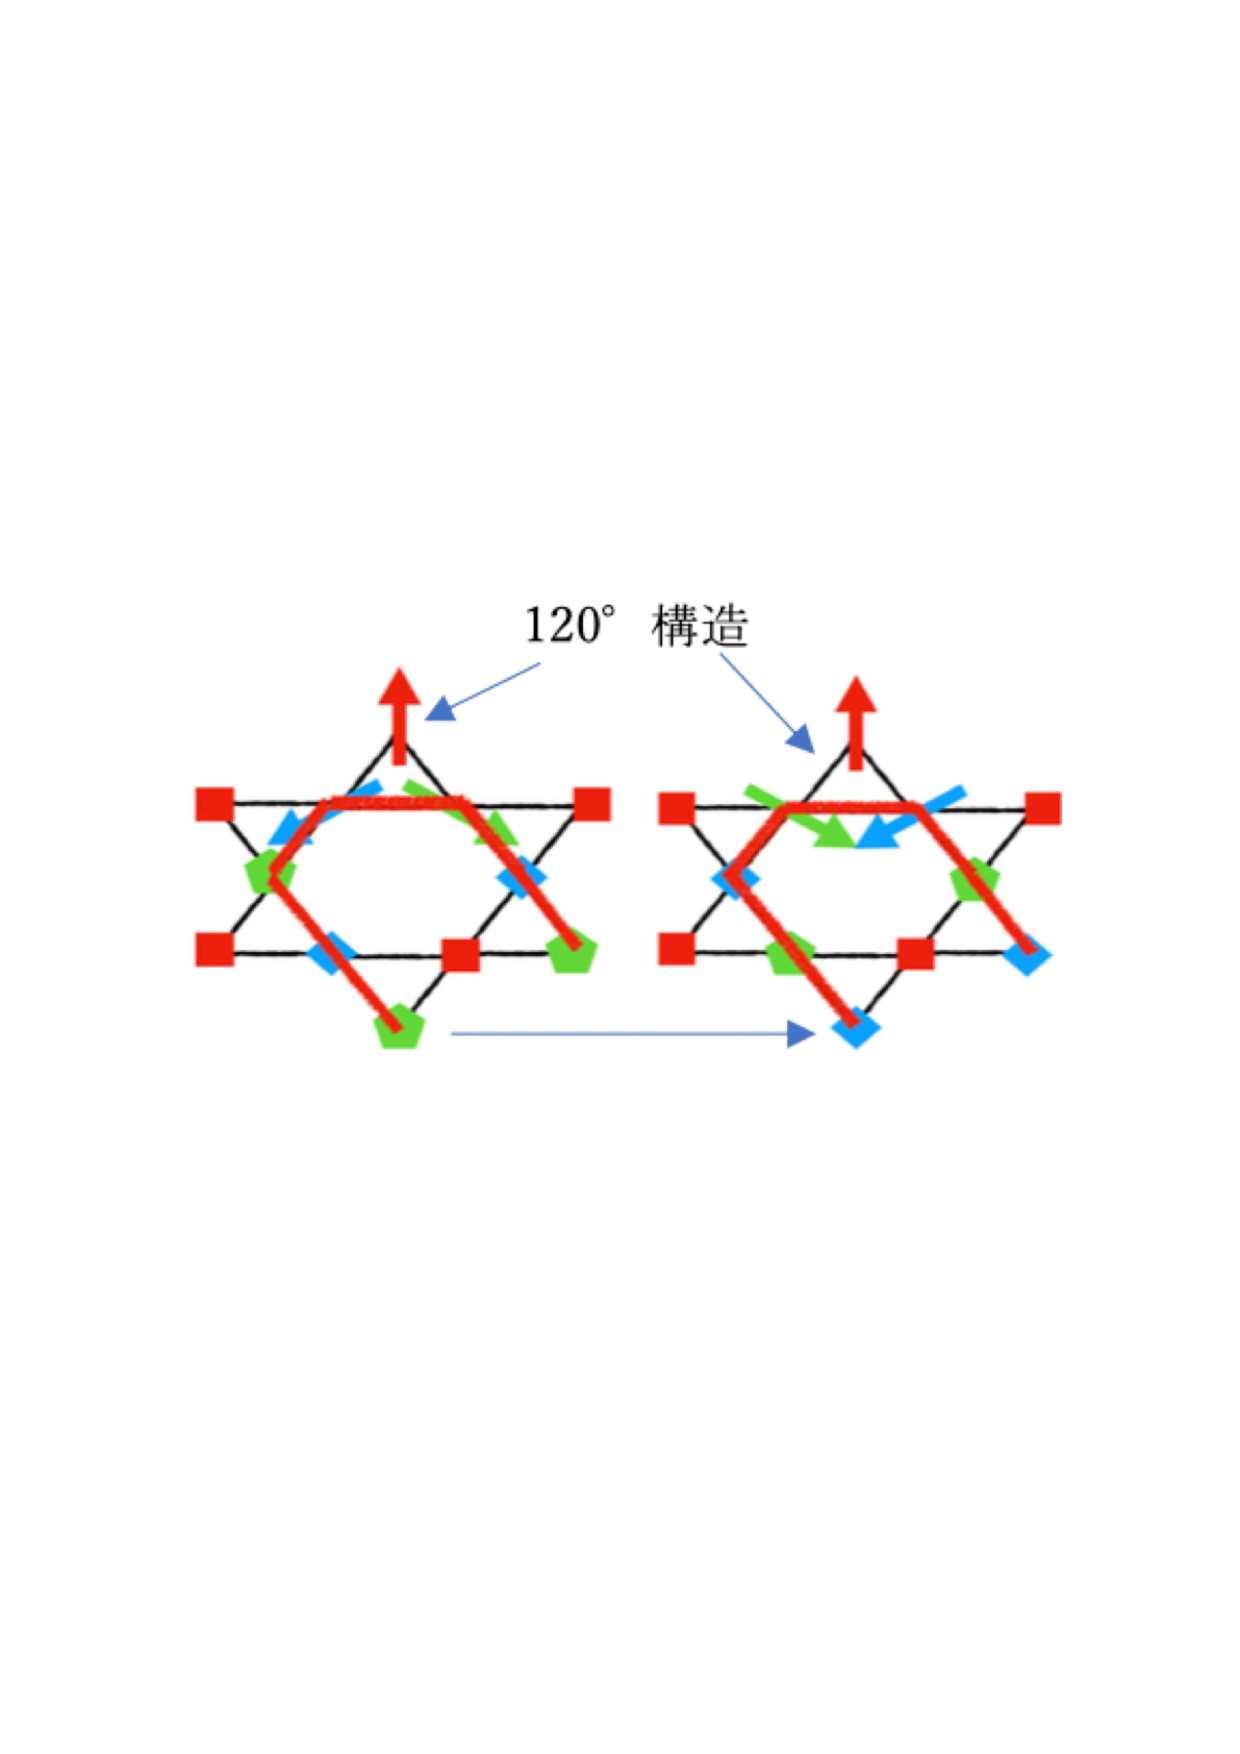
\includegraphics[width=10cm]{figure/loop_update.pdf}
   \caption{ループアップデートの概念図}
\end{figure}

\newpage

%\section{非平衡緩和法}
\subsection{非平衡緩和法}

%\subsection{計算する物理量}
\subsubsection{計算する物理量}
非平衡緩和法では以下で定義される秩序変数$O$の時間相関関数$G_O(t)$を計算する。
\begin{align}
   G_{O}(t) \equiv \ev{O(t) \cdot O(0)}.
\end{align}
時刻$t$は1MC stepを単位に測る。
1MC stepはすべてのスピンに対して一度シングススピンフリップアップデートを試行することと定義する。
$O(t)$は時刻$t$における秩序変数$O$の値を表す。
$\ev{\cdots}$はサンプル平均で、システムサイズが有限であることに起因するゆらぎを抑制するためにとる。
非平衡緩和法は$G_O(t)$の時間変化(緩和過程)から転移温度$T_{\mathrm{c}}$を推定する手法である。
%熱力学平均$\ev{O}$を計算しない、すなわち平衡分布への収束を必要としないため、平衡法に比べて大きなサイズの系を扱うことができる。

%\subsection{非平衡緩和法の一般論}
\subsubsection{非平衡緩和法の一般論}

$T>T_{\mathrm{BKT}}$では$G(t)$は指数関数的に減衰すると期待される。(空間相関関数からの類推)
\begin{align}
   G(t) =  a \ \mathrm e^{-t/\tau}.
\end{align}
$\tau$を緩和時間という。両辺の対数を取ると
\begin{align}
   \ln{G(t)} = \ln{a}-\frac{1}{\tau}t.
\end{align}
$\ln{G(t)}$から$\tau$を推定する。
$\tau$の温度依存性は転移温度近傍$T\sim T_{\mathrm{BKT}}$で
\begin{align}
   \tau = b \ \exp [c/(T-T_{\mathrm{BKT}})^{1/2}].
\end{align}
同じく両辺の対数を取って
\begin{align}
   \ln{\tau} = \ln{b} + \frac{c}{\sqrt{T-T_{\mathrm{BKT}}}}.
\end{align}
$\ln{\tau}$から$T_{\mathrm{BKT}}$を推定する\cite{Levenberg1944method,Marquardt1963algorithm}。
以下に示す二つの図が非平衡緩和法の典型的な結果である(二次元正方格子上の$XY$模型\cite{Ozeki2003})。
%\cite{Ozeki2003}で行われた二次元正方格子上の$XY$模型に対する非平衡緩和法の結果を示す。
ただし、$m(t)$は
\begin{align}
   m(t) \equiv \frac{1}{N}\sum_i\ev{\cos{\qty[\theta_i(t) - \theta_i(0)]}}
\end{align}
で、$G(t)$に対応する。$N$は格子点数、$\theta_i$は格子点$i$のスピンを$x$軸から測った角度である。
%カイラリティ転移の場合、転移温度近傍での$\tau$の温度依存性のみBKT転移と異なる。
%\begin{align}
%   \tau = b \ (T-T_{\mathrm{c}})^{-z\nu}.
%\end{align}
%
%本研究ではスケーリング則を利用し複数温度の$G(\tau)$から$\tau$を同時に推定する。

\begin{figure}[H]
   \begin{minipage}{0.5\hsize}
    \begin{center}
     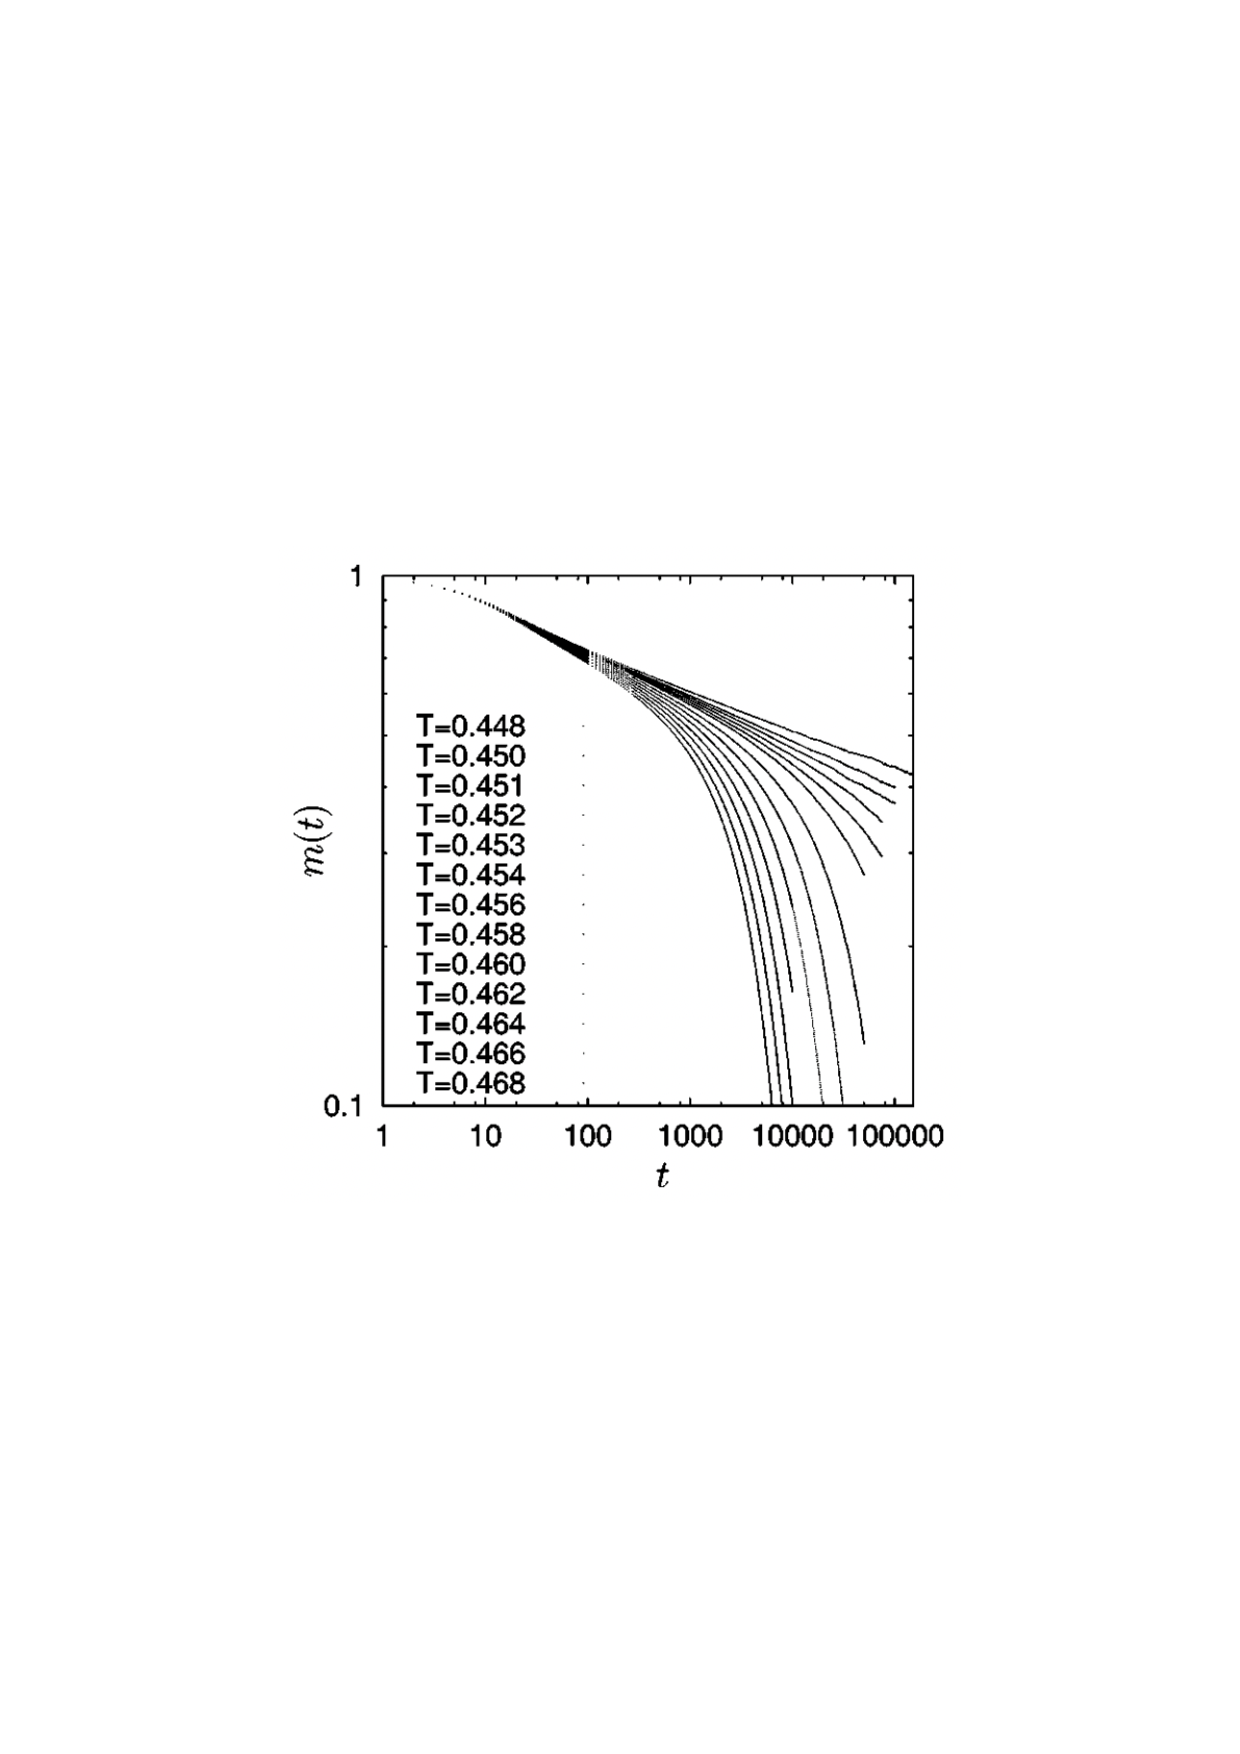
\includegraphics[width=7.5cm]{figure/typical_Gt.pdf}
    \end{center}
    \caption{磁気秩序変数の時間相関関数}
    %\label{fig:one}
   \end{minipage}
   \begin{minipage}{0.5\hsize}
    \begin{center}
     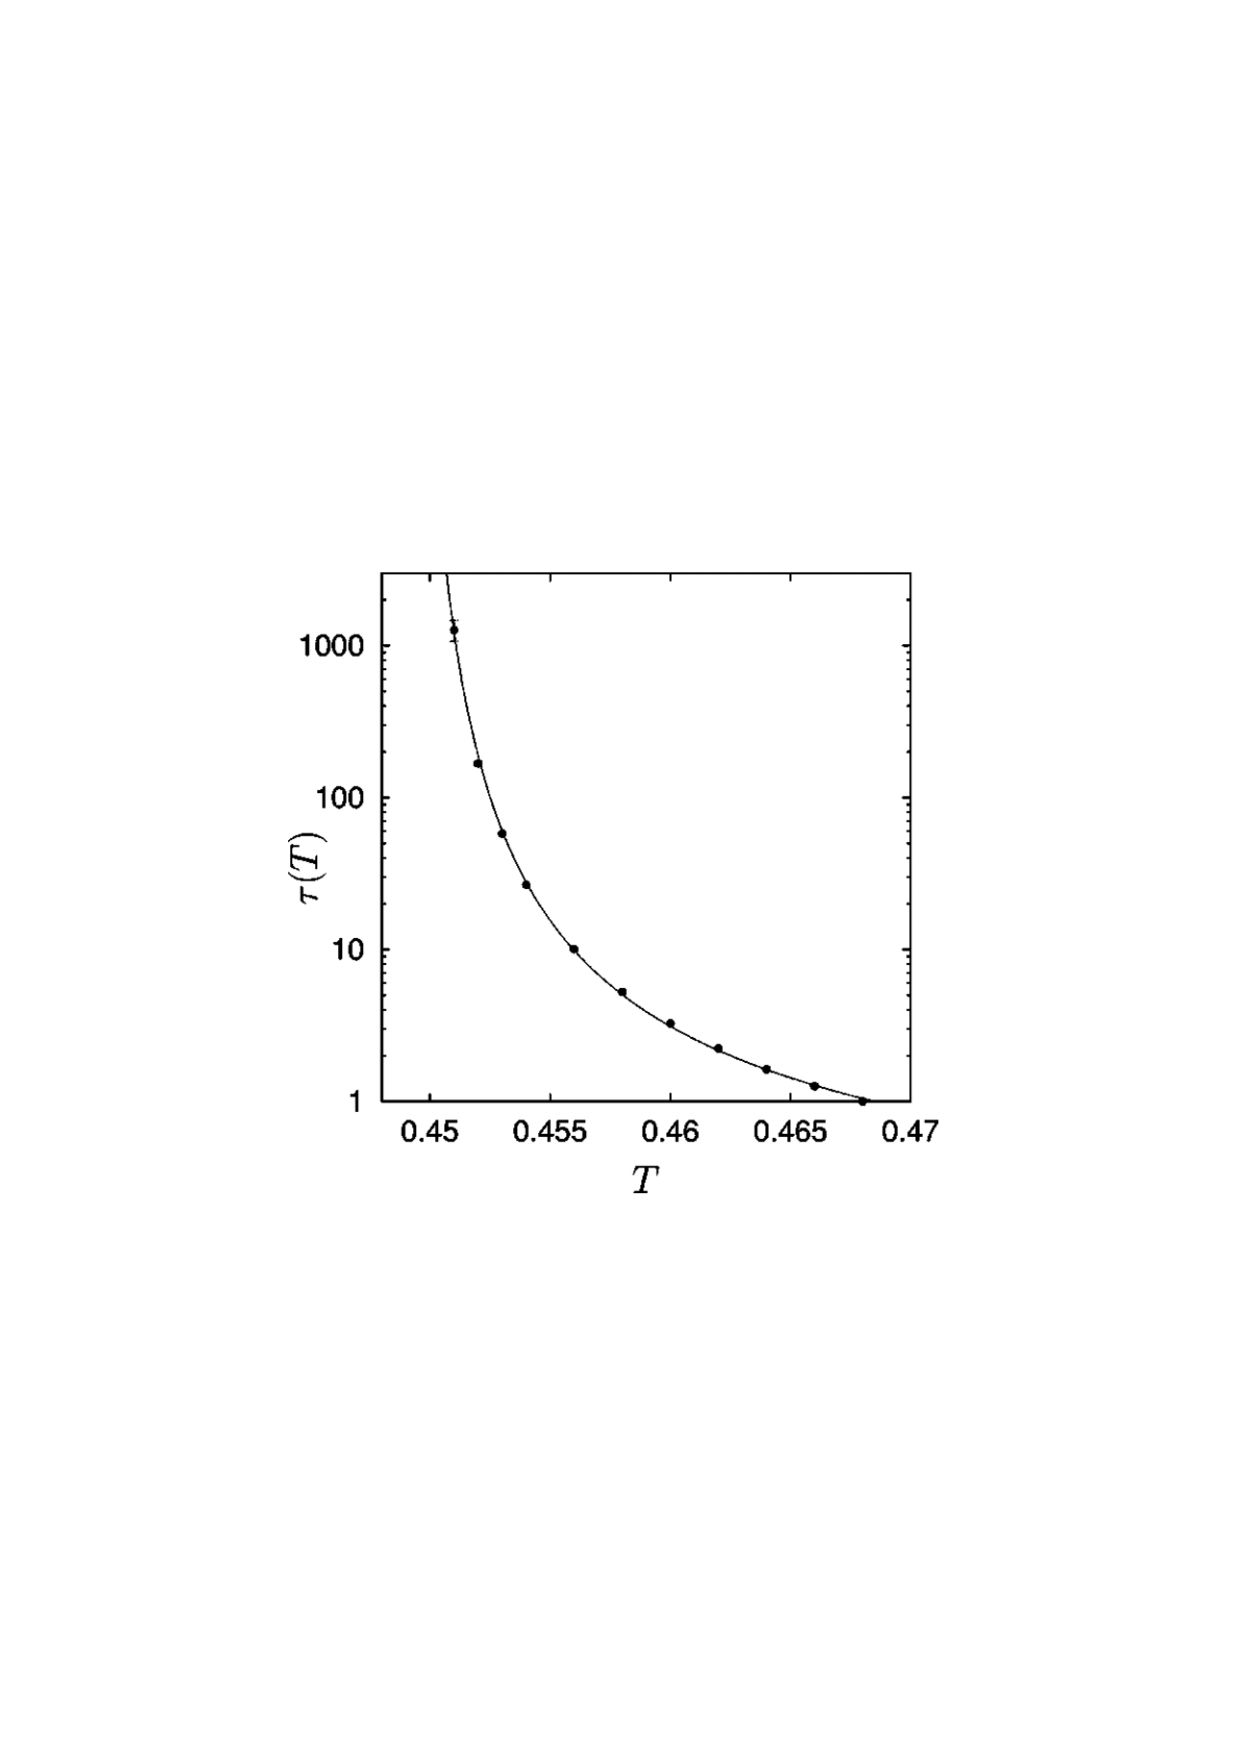
\includegraphics[width=7.5cm]{figure/typical_relaxation_time.pdf}
    \end{center}
    \caption{緩和時間の温度依存性}
    %\label{fig:two}
   \end{minipage}
\end{figure}

カイラリティ転移の場合、転移温度近傍での$\tau$の温度依存性のみBKT転移と異なる。
\begin{align}
   \tau = b \ (T-T_{\mathrm{c}})^{-z\nu}.
\end{align}

本研究ではスケーリング則を利用し複数温度の$G(\tau)$から$\tau$を同時に推定する。

%\newpage

%\subsection{スケーリング則を利用した緩和時間の推定}
\subsubsection{スケーリング則を利用した緩和時間の推定}

$T>T_{\mathrm{BKT}}$において、各温度の$G(t)$は以下のスケーリング則に従うと期待される\cite{Ozeki2003}。
\begin{align}
   g(t/\tau) = \tau_{\mathrm{exact}}^{\lambda}G(t).
\end{align}
$\tau_{\mathrm{exact}}$は厳密な緩和時間、$\lambda$は$G(t)$の動的臨界指数を表す。
%$\lambda$は時間と温度に依存しないと仮定する[動的臨界指数だとすると、by definiton?]
この式によると、$T>T_{\mathrm{BKT}}$において、各温度の$G(t)$と$\tau_{\mathrm{exact}}$から計算される
$\tau_{\mathrm{exact}}^{\lambda}G(t)$はすべての温度で一致する。
したがって、$\tau^{\lambda}G(t)$が一致するように$\tau$を最適化すれば$\tau\sim\tau_{\mathrm{exact}}$が得られると期待される。
カイラリティ転移の場合も同様の手続きで解析する。
\begin{itembox}[1]{スケーリング則を利用した緩和時間$\tau$の推定アルゴリズム}
   \begin{enumerate}
       %\item 解析に用いる温度列[T_1,T_2,\cdots,T_n]を選び、適当な初期配列[\tau_1,\tau_2,\cdots,\tau_n]を用意する。
       \item 計算結果$\vec{G}(t)=[G_1(t),G_2(t),\cdots,G_n(t)]$から、計算に用いる温度を選ぶ。
       \item 適当な初期配列$\vec{\tau}=[\tau_1,\tau_2,\cdots,\tau_n]$を用意する。$n$は温度の点数を表す。
       \item $\vec{G}(t)$と$\vec{\tau}$から$\vec{g}(t,\vec{\tau})=[g_1(t/\tau_1),g_2(t/\tau_2),\cdots,g_n(t/\tau_n)]$を構成する。
       \item $\vec{g}(t,\vec{\tau})$を時刻$t$について内挿し、$g_{\mathrm{mean}} = \qty(1/n) \sum_n g_n(t/\tau_n)$を計算する。
       \item $\sum_n \norm{\vec{g}(t,\vec{\tau})-g_{\mathrm{mean}}}^2/\norm{g_{\mathrm{mean}}}^2$が最小となるように$\vec{\tau}$を最適化する\cite{10.1093/comjnl/7.4.308}。
   \end{enumerate}
\end{itembox}
%[$\lambda$の扱いについて説明する。・$\lambda$も変分パラメータに含めたこと・その理由(動的臨界指数の値を知らない)・動的臨界指数の普遍性からおそらく時間/温度依存性がないと期待されること]
\newpage

\section{結果}
\subsection{$J_2-T$相図}
本研究で作成した数値的な$J_2-T$相図を示す。
$q=0$相の相境界を比熱のピーク温度から、それ以外を非平衡緩和法によって決定した。
大域的な相構造は先行研究と整合するが、$-7\times10^{-2}\le J_2/J_1\le -7.5\times10^{-3}$に報告のない明確な一次転移が存在する。
また、八極子相は報告よりも広い$-5\times10^{-3}<J_2/J_1\le2\times10^{-2}$に存在する。
さらに、一次転移の低温側の臨界終点は$q=0$相・八極子相・常磁性相の相境界に近接している。
これは低温での一次転移消失と八極子相の存在の間の関係を示唆している。
また、$J_2=0.02$において$2\times10^{-3}\si{\kelvin}$程度のカイラリティ転移と$\sqrt{3}\times\sqrt{3}$秩序のBKT転移の転移温度分離が確認された。
原点近傍の複雑な相構造は極低温における更新凍結によって確認されなかった。
%\begin{itemize}
%   \item 本研究で作成した数値的$J_2-T$相図を示す。
%   \item $q=0$相の相境界を比熱のピーク温度から、それ以外を非平衡緩和法によって決定した。
%   \item 大域的な相構造は先行研究と整合する。
%   \item 八極子相は先行研究の報告よりも広い$-5\times10^{-3}<J_2/J_1\le2\times10^{-2}$に存在する。
%   \item $-7\times10^{-2}\le J_2/J_1\le -7.5\times10^{-3}$に報告のない明確な一次転移?が存在する。
%   \item この一次転移?の低温側の臨界終点は$q=0$相・八極子相・常磁性相の相境界に近接している。(これは低温での一次転移消失と八極子相の存在の間の関係を示唆している。)
%   \item 極低温における更新凍結によって原点近傍の複雑な相構造を確認できなかった。
%   \item 
%\end{itemize}
\begin{figure}[H]
   \centering
   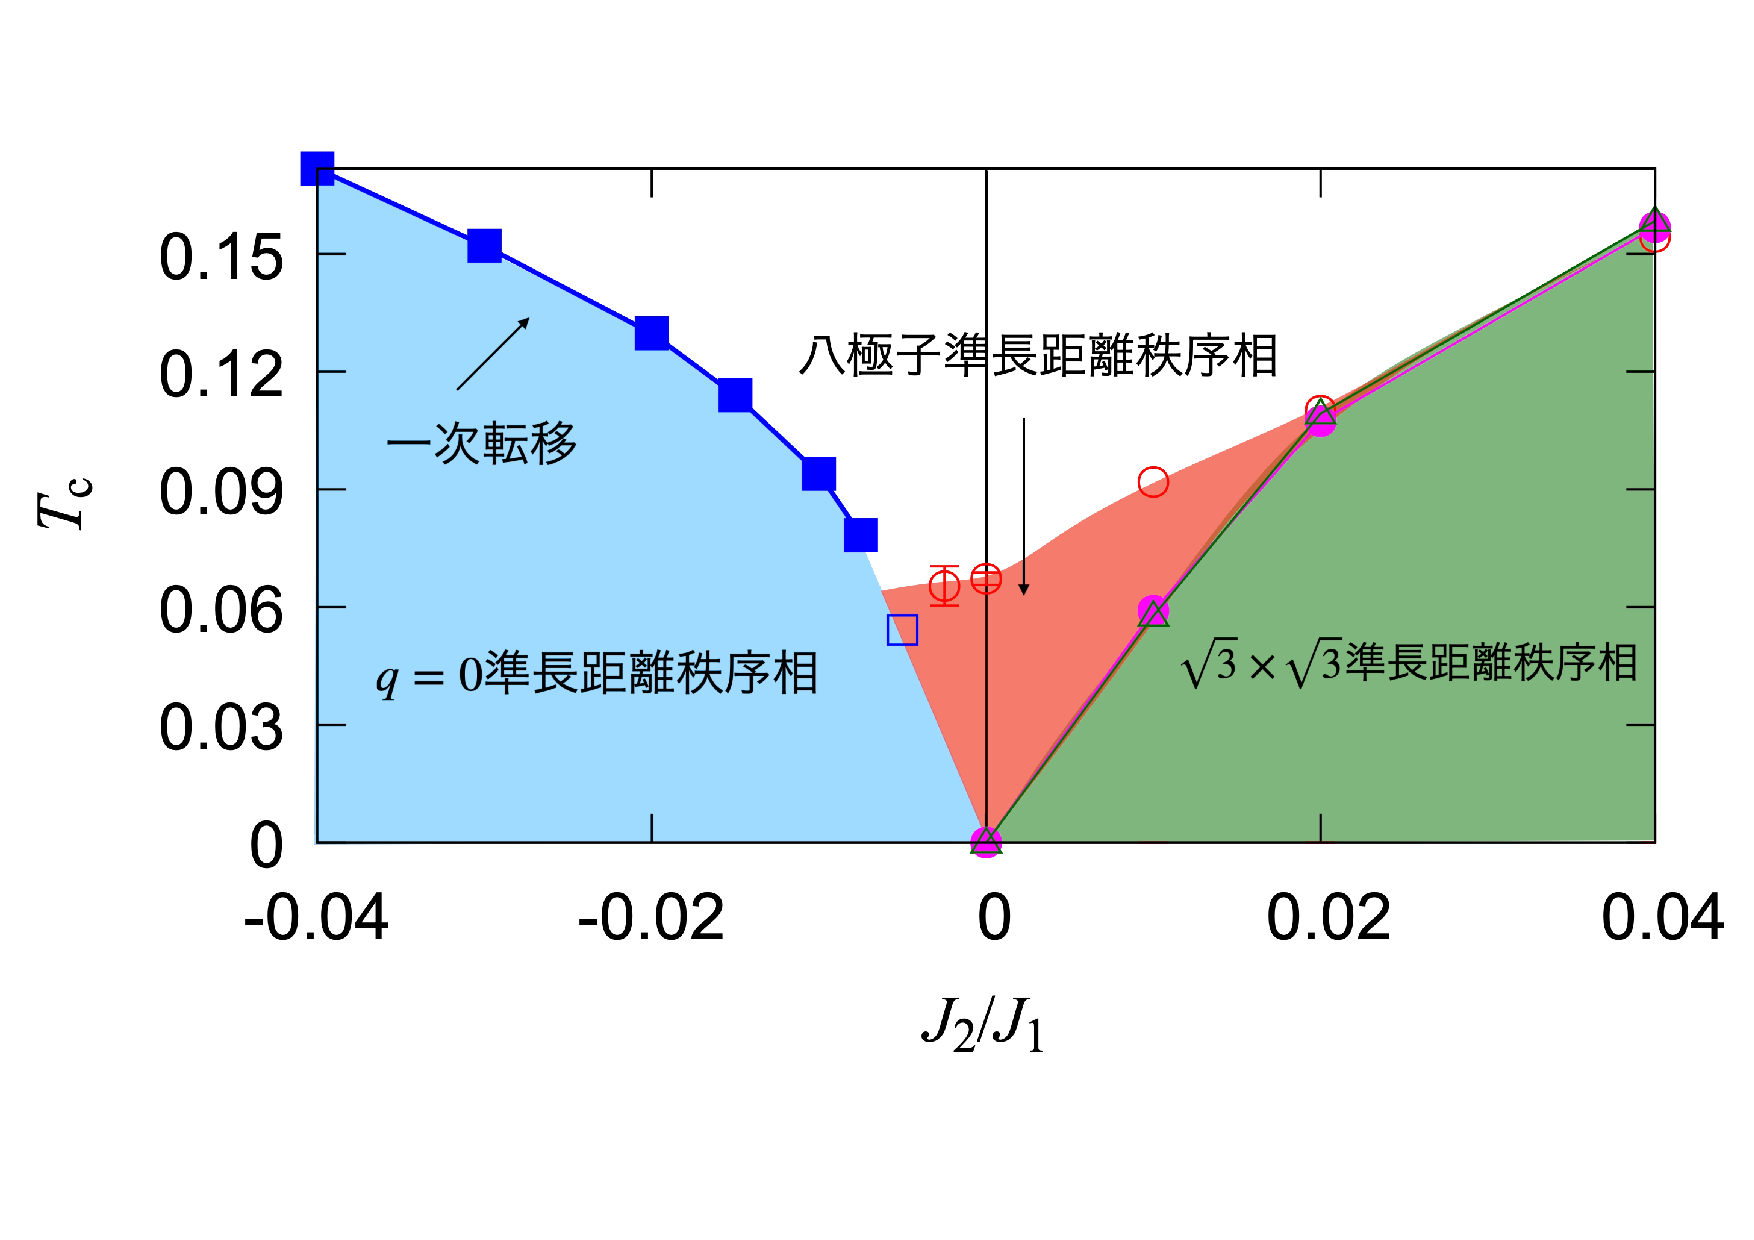
\includegraphics[width=15cm]{figure/phase_diagram_broad.pdf}
   \caption{$J_2-T$相図}
\end{figure}

%\begin{figure}[H]
%   \centering
%   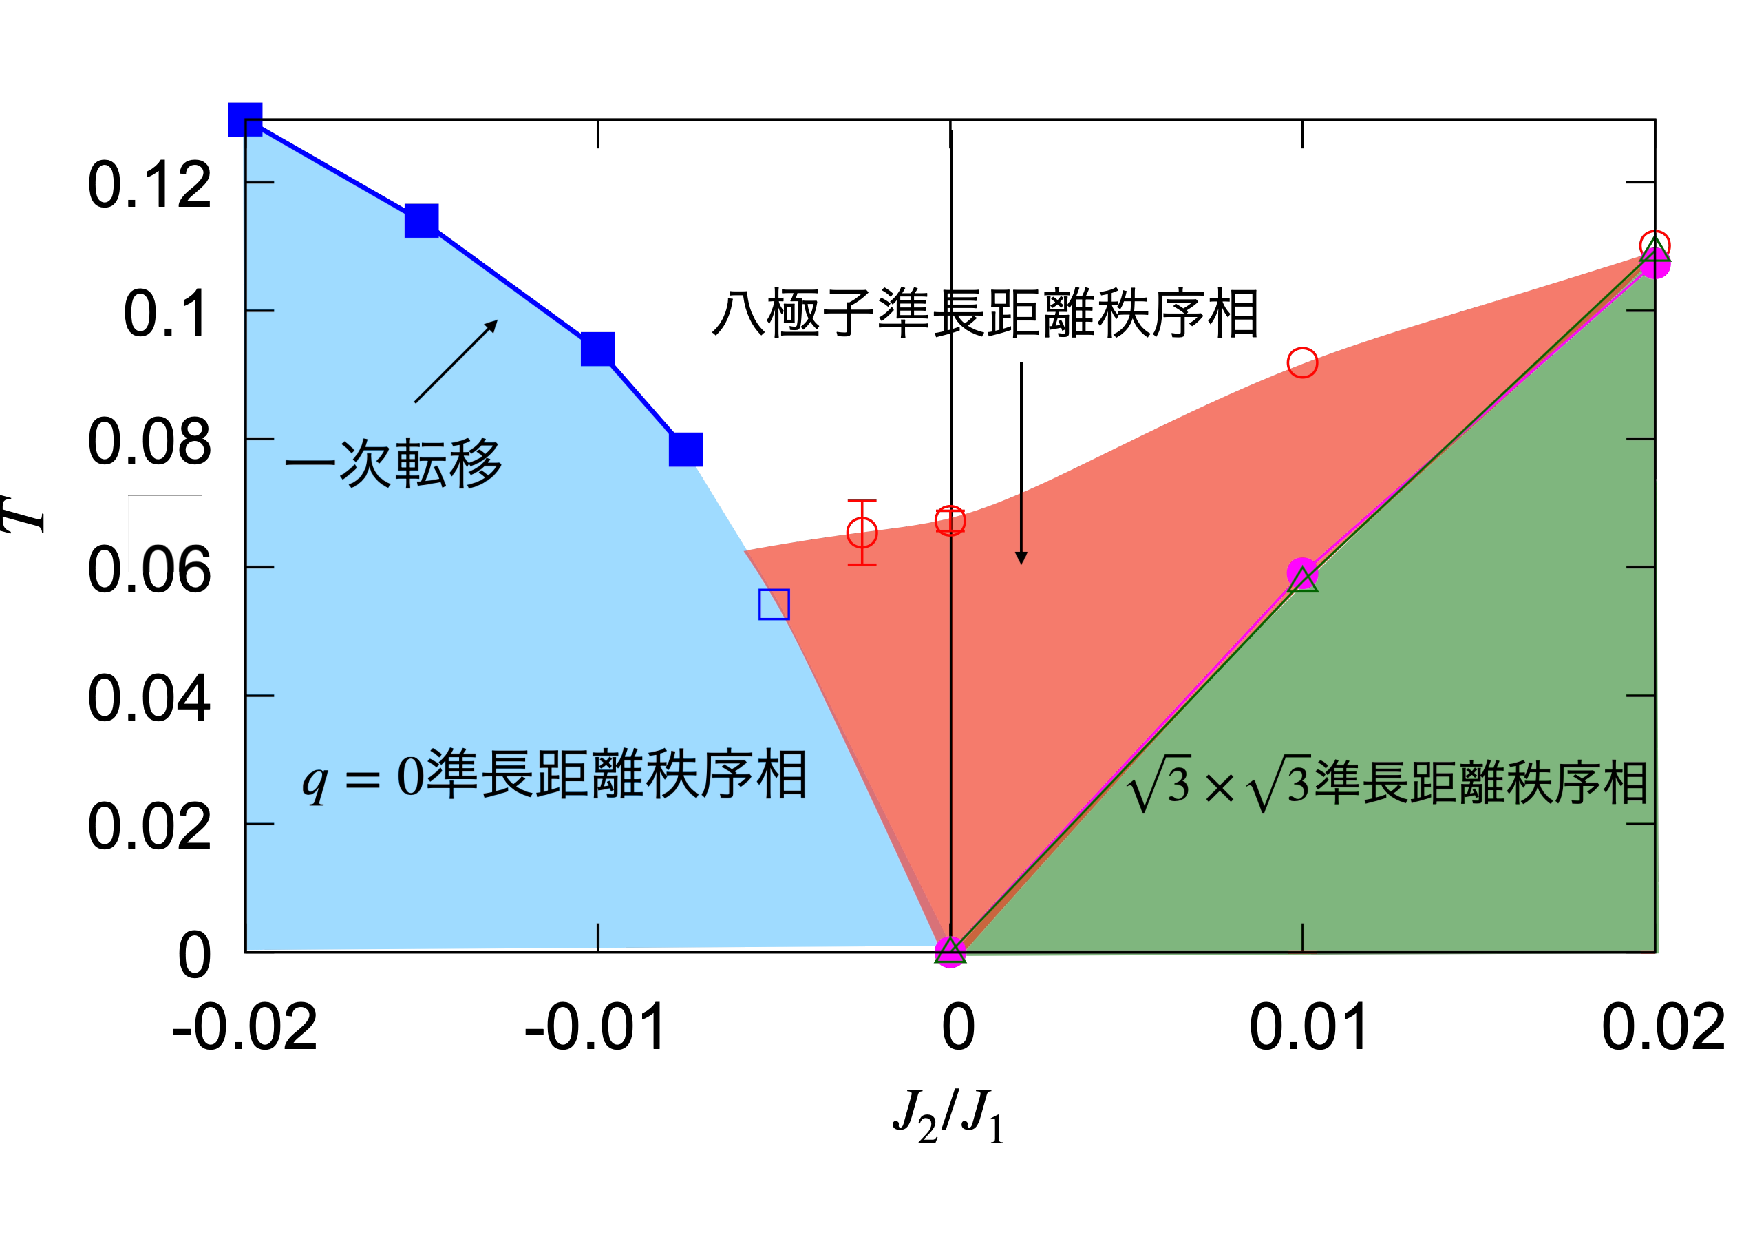
\includegraphics[width=15cm]{figure/phase_diagram.pdf}
%   \caption{$J_2-T$相図}
%\end{figure}

\subsection{比熱}
代表的な$J_2$における比熱の温度とサイズ依存性を示す。
まず、$J_2=-3\times10^{-2}$の比熱はサイズ増加とともに増大する鋭いピークを示す。  
これはこの転移が一次転移であることを強く示唆している。
$J_2=-5\times10^{-3}$の比熱は他の二点と異なり、二つのピークを持つ。
高温側の転移は常磁性--八極子転移、低温側は八極子--$q=0$転移に対応する。
高温側のピークはサイズの増加に伴って減少し、それとは対照的に、低温側のピークは増大する。
サイズ依存性から明らかに、高温側の転移は一次転移ではない。
低温側の転移が一次転移か否かは、低温での一次転移消失と八極子相の関係を調べる上で重要であるが、比熱のデータからは断定できない。
最後に、$J_2=4\times10^{-2}$の比熱は他の二点に比べてサイズ依存性が小さく、緩やかなピークを示す。
これはこの転移が連続転移であることを示唆している。

$J_2=-5\times10^{-3}$の低温側の転移が一次転移か否かを調べるため、比熱のピークのシステムサイズに対するスケーリング解析を行った。
必要に応じて各$J_2$で大サイズ系を数点追加計算した。
一次転移であれば、$L\to\infty$で$C_{\mathrm{peak}}^{-1}$が$L^{-2}$に対して線形となることが知られている\cite{baumgartner2012monte}。
実際、一次転移が強く示唆された$J_2=-3\time10^{-2}$の傾向は$y=x$に一致する。
また、連続転移が示唆された$J_2=4\times10^{-2}$の傾向は明らかに$y=x$に一致しない。
しかし、スケーリング解析によっても$J_2=-5\times10^{-3}$の低温側の転移が一次転移であるか断定できない。

%最後に、エネルギーギャップの$J_2$依存性を調べ、一次転移領域で確認されたエネルギーギャップが$J_2\to 0$でどのように閉じていくかを調べた。
%
%また、$J_2=-0.1$と$J_2=-7\times10^{-2}$のデータから

%\begin{itemize}
%   \item 代表的な$J_2$における比熱の温度とサイズ依存性を示す。
%   \item $J_2=-3\times10^{-2}$の比熱のピークは
%   \item $J_2=-5\times10^{-3}$の比熱は
%   \item 最後に、$J_2=4\times10^{-2}$の比熱は他の二点に比べてピークがブロードで、サイズ依存性が小さい。
%   \item これは$J_2=4\times10^{-2}$の比熱は他の二点に比べてピークがブロードで、サイズ依存性が小さい。
%   \item これは
%\end{itemize}

\begin{figure}[H]
   \centering
   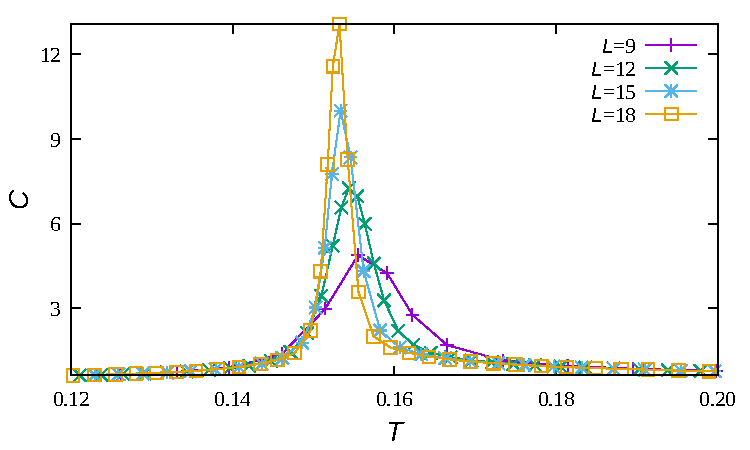
\includegraphics[width=12cm]{figure/c_j2_-3e-2.pdf}
   \caption{$J_2=-0.03$における比熱の温度とサイズ依存性}
\end{figure}

\begin{figure}[H]
   \centering
   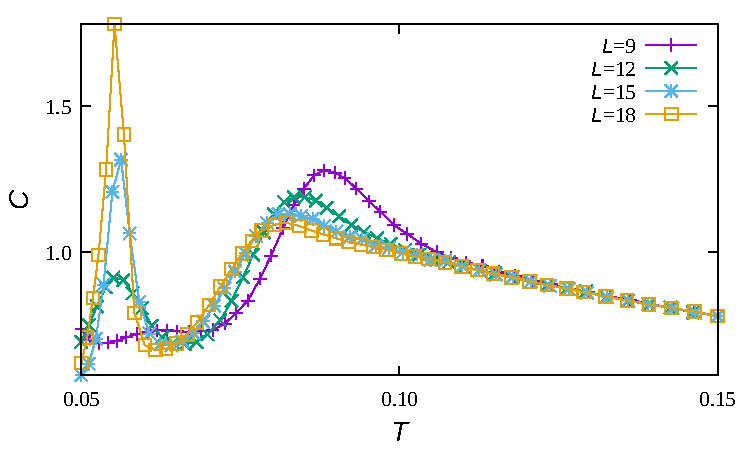
\includegraphics[width=12cm]{figure/c_j2_-5e-3.pdf}
   \caption{$J_2=-0.005$における比熱の温度とサイズ依存性}
\end{figure}

\begin{figure}[H]
   \centering
   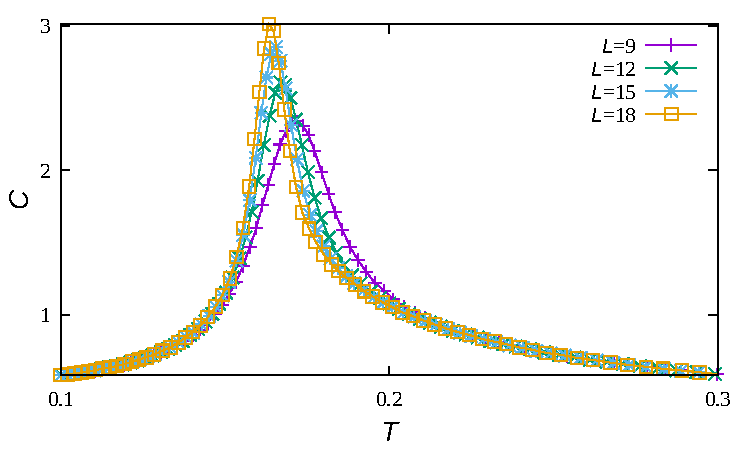
\includegraphics[width=12cm]{figure/c_j2_4e-2.pdf}
   \caption{$J_2=0.04$における比熱の温度とサイズ依存性}
\end{figure}

%\begin{figure}[H]
%   \centering
%   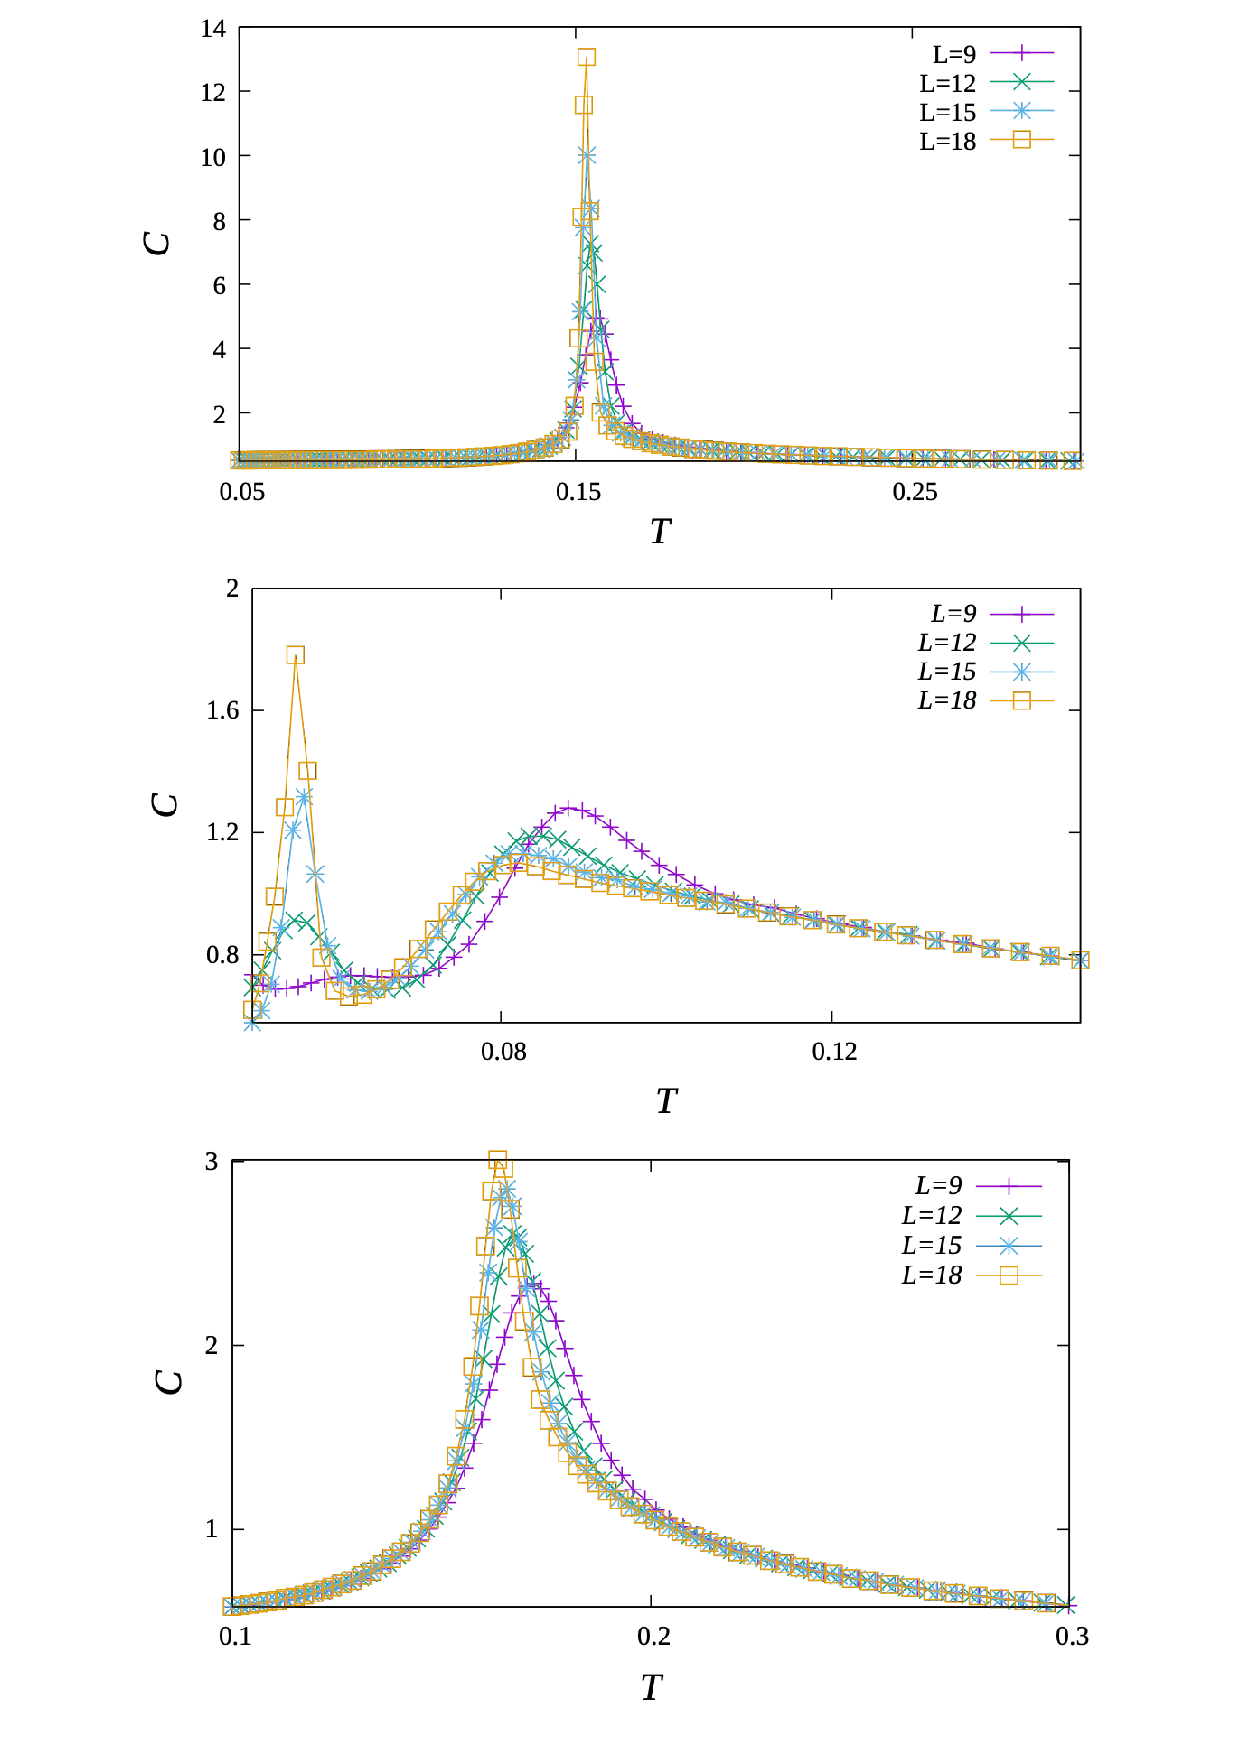
\includegraphics[width=15cm]{figure/specific_heat.pdf}
%   \caption{比熱の温度とサイズ依存性}
%\end{figure}

\begin{figure}[H]
   \centering
   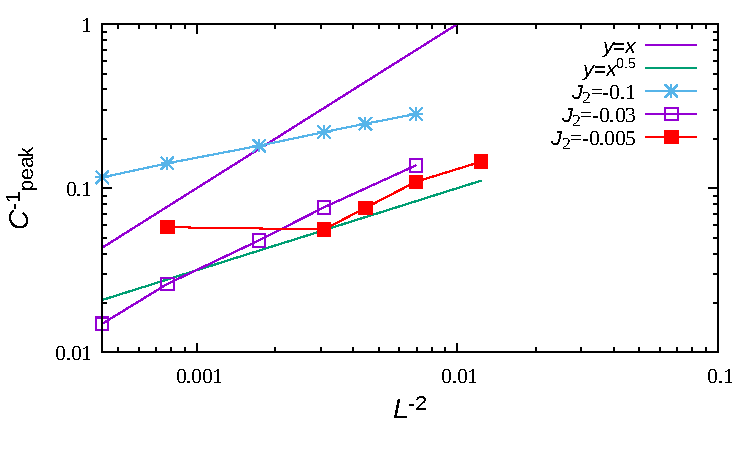
\includegraphics[width=12cm]{figure/scaling_c.pdf}
   \caption{比熱ピークのスケーリング}
\end{figure}

\newpage

\subsection{エネルギーヒストグラム}
$J_2<0$における一次転移領域を明らかにするため、各$J_2$でエネルギーヒストグラムを作成した。
温度は比熱がピークをとる温度を選んだ。
一般に、一次転移領域においてエネルギーヒストグラムはダブルピーク構造を示す。
そこで、各エネルギーヒストグラムを非線形項込みのシングルガウシアンピーク
\begin{align}
   f(x)  = h_1\exp\qty[-\qty{(x-c_1)/w_1}^2 + a_1\qty{(x-c_1)/w_1}^3 + b_1\qty{(x-c_1)/w_1}^4]
\end{align}
と非線形項込みのダブルガウシアンピーク
\begin{align}
   g(x) &= h_1\exp\qty[-\qty{(x-c_1}/w_1)^2 + a_1\qty{(x-c_1)/w_1)}^3 + b_1\qty{(x-c_1}/w_1)^4] \nonumber\\ 
        &+ h_2\exp\qty[-\qty{(x-c_2}/w_2)^2 + a_2\qty{(x-c_2)/w_2)}^3 + b_2\qty{(x-c_2}/w_2)^4]
\end{align}
でフィッティングした。以下、単にシングル(ダブル)ガウシアンピークと省略する。
また、ダブルガウシアンピークフィッティングの結果からエネルギーギャップを計算し、その$J_2$依存性を調べた。
下に代表的な$J_2$におけるエネルギーヒストグラムを示す。

まず、$J_2=-0.1$はデータ自体のゆらぎが大きいピーク近傍を除いてシングルガウシアンピークとダブルガウシアンピークの両方でよくフィッティングできる。これは$J_2=-0.1$における転移が一次転移でないことを示唆しており、$C^{-1}_{\mathrm{peak}}-L^{-2}$スケーリングの結果と一致する。

次に、$J_2=-7\times10^{-2}$において、ごく僅かであるが、$E\sim-0.895$にシングルガウシアンピークではフィッティングできない構造が存在する。
また、ヒストグラムのピークもシングルガウシアンピークではフィッティングできていない。
これは一次転移の高温側の終点が$J_2=-7\times10^{-2}$近傍に存在することを示唆している。
一方で、有限サイズ効果によって$J_2\le-7\times10^{-2}$でもエネルギーギャップが有限に残る。
そのため、一次転移の高温側終点を精密に決定するのは難しいと考えられる。

最後に、$J_2=-7.5\times10^{-3}$は他二点に見られない顕著なダブルピーク構造を示す。
$E\sim-0.96$にダブルガウシアンピークでもフィッティングできない構造があるが、シングルガウシアンピークでは完全にフィッティングできない。
よって、$J_2=-7.5\times10^{-3}$の転移は一次転移である。
また、$J_2<-7.5\times10^{-3}$でダブルピーク構造は確認されなかった。
したがって、一次転移の低温側の終点は$J_2=-7.5\times10^{-3}$近傍に存在する。

以上を踏まえて、エネルギーギャップの$J_2$依存性を整理する。
まず、一次転移の低温側終点である$J_2=-7.5\times10^{-3}$から$J_2=-2\times10^{-2}$まで$\abs{J_2}$の増加とともに$\Delta E$が単調に増加する。
対照的に、$J_2=-2\times10^{-2}$から一次転移の高温側終点である$J_2=-7.5\times10^{-3}$まで$\abs{J_2}$の増加とともに$\Delta E$が単調に減少する。
最後に、$J_2<-7\times10^{-2}$では一次転移性を示さないが、有限サイズ効果によって$\Delta E$が有限に残る。


\begin{figure}[H]
   \centering
   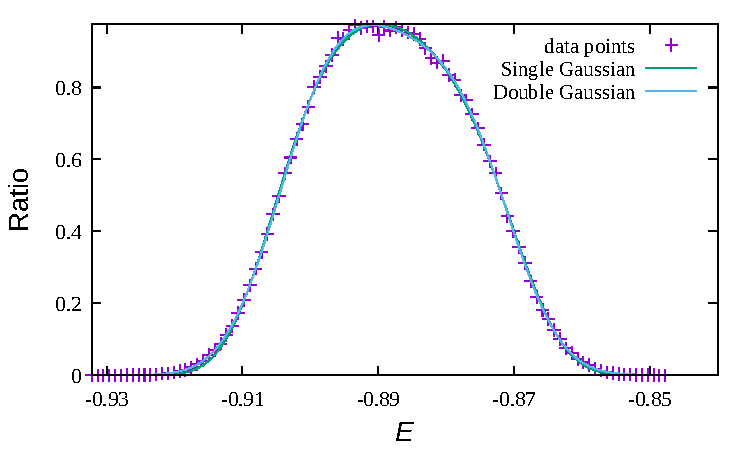
\includegraphics[width=12cm]{figure/energy_histogram_j2_-1e-1.pdf}
   \caption{$J_2=-0.1$のエネルギーヒストグラム}
\end{figure}

\begin{figure}[H]
   \centering
   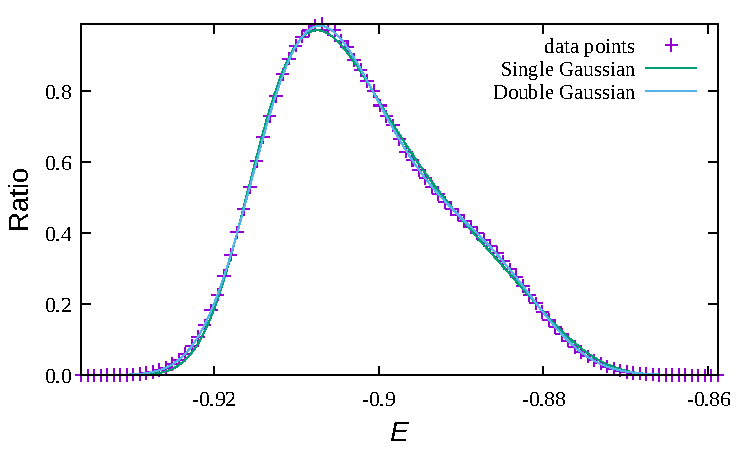
\includegraphics[width=12cm]{figure/energy_histogram_j2_-7e-2.pdf}
   \caption{$J_2=-7\times10^{-2}$のエネルギーヒストグラム}
\end{figure}

\begin{figure}[H]
   \centering
   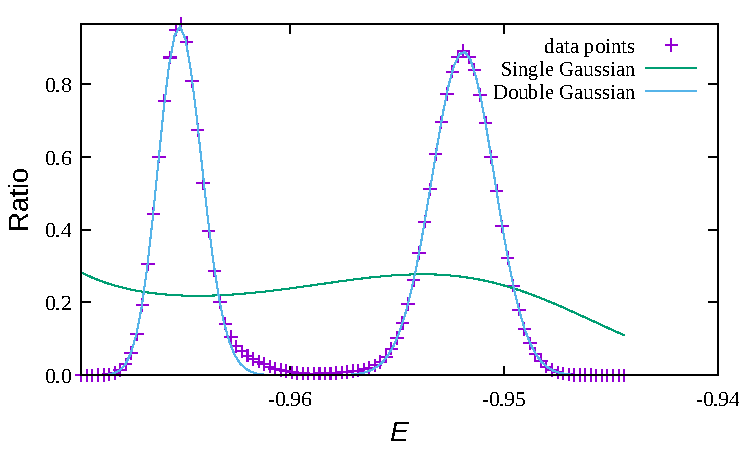
\includegraphics[width=12cm]{figure/energy_histogram_j2_-7.5e-3.pdf}
   \caption{$J_2=-7.5\times10^{-3}$のエネルギーヒストグラム}
\end{figure}

\begin{figure}[H]
   \centering
   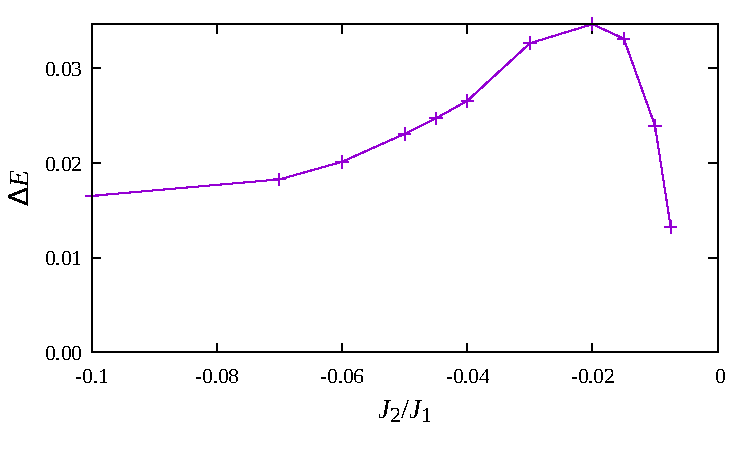
\includegraphics[width=12cm]{figure/energy_gap.pdf}
   \caption{エネルギーギャップの$J_2$依存性}
\end{figure}

%\begin{figure}[H]
%   \centering
%   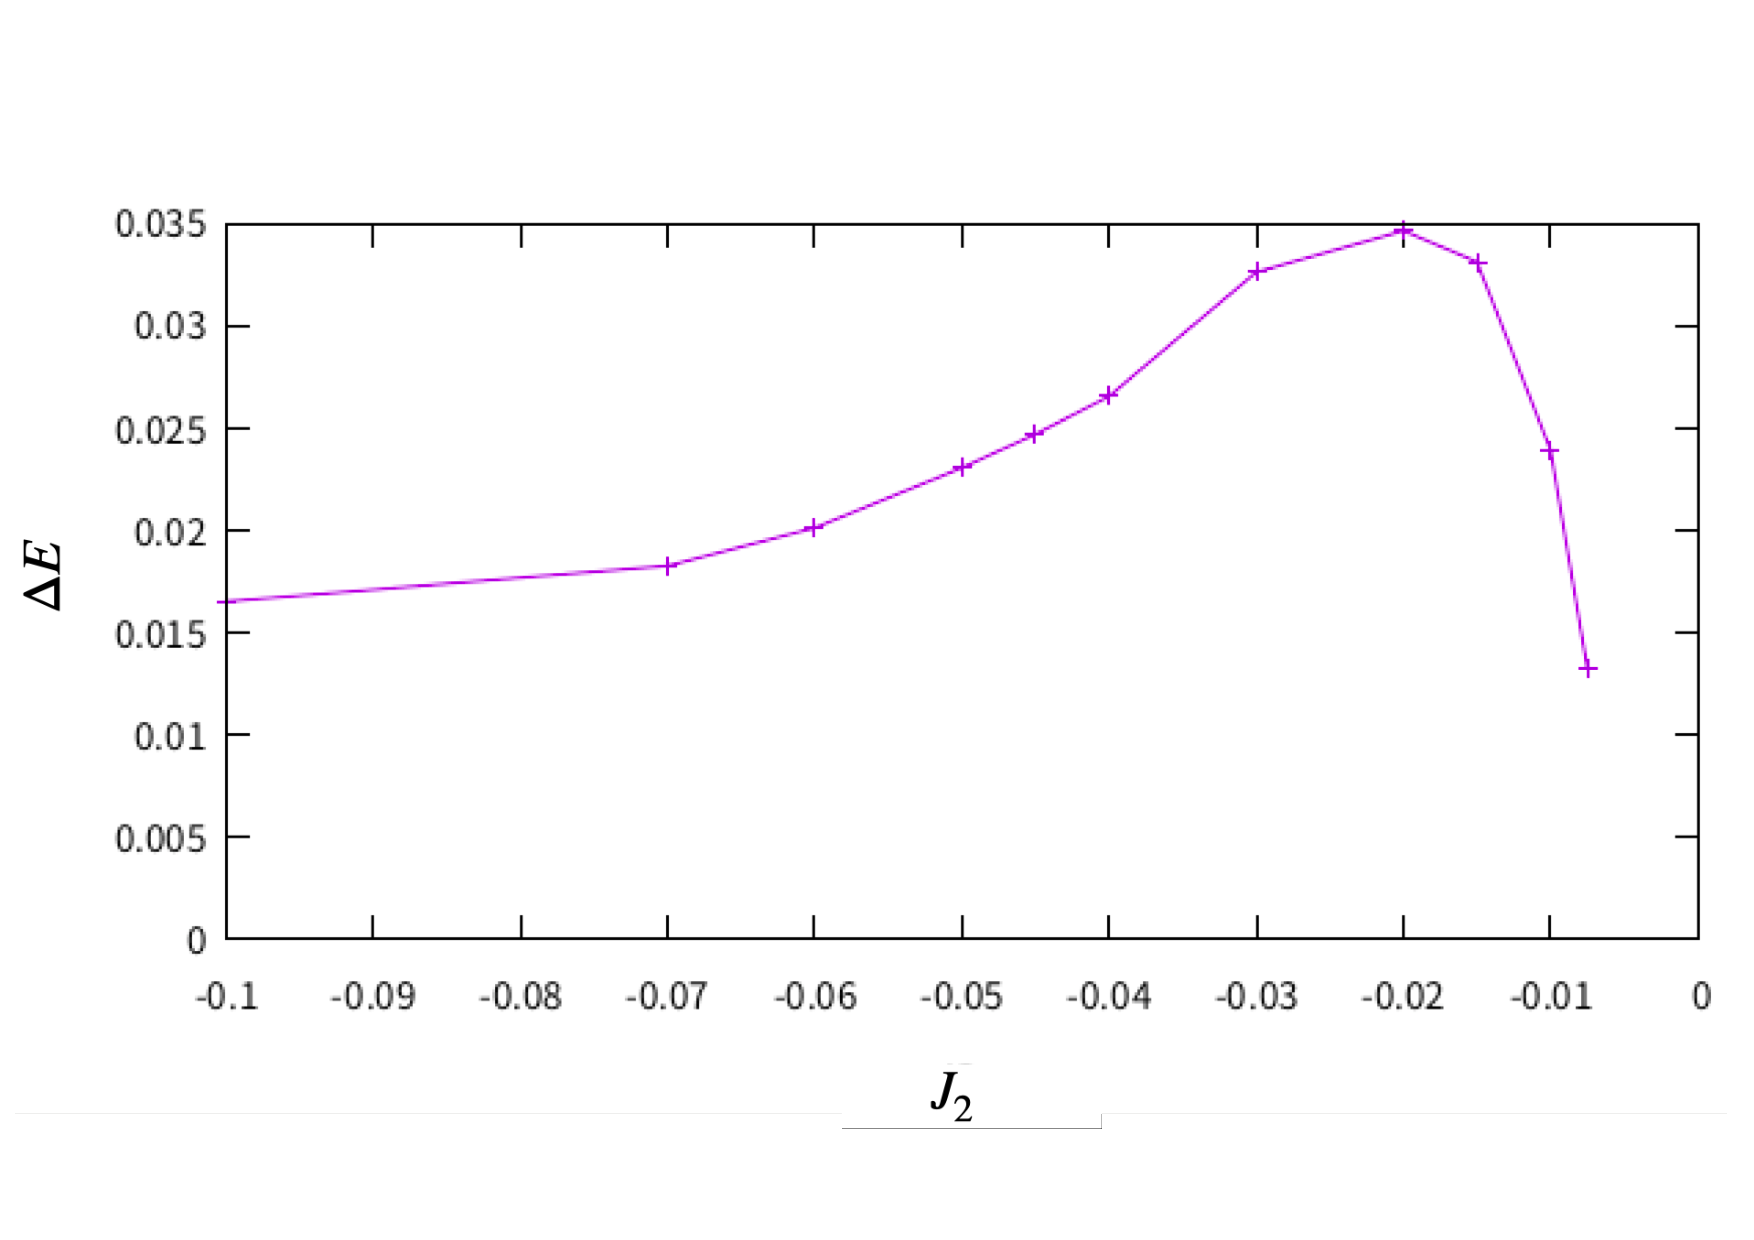
\includegraphics[width=15cm]{figure/egap_j2.pdf}
%   \caption{エネルギーギャップの$J_2$依存性}
%\end{figure}
%
%\begin{figure}[H]
%   \centering
%   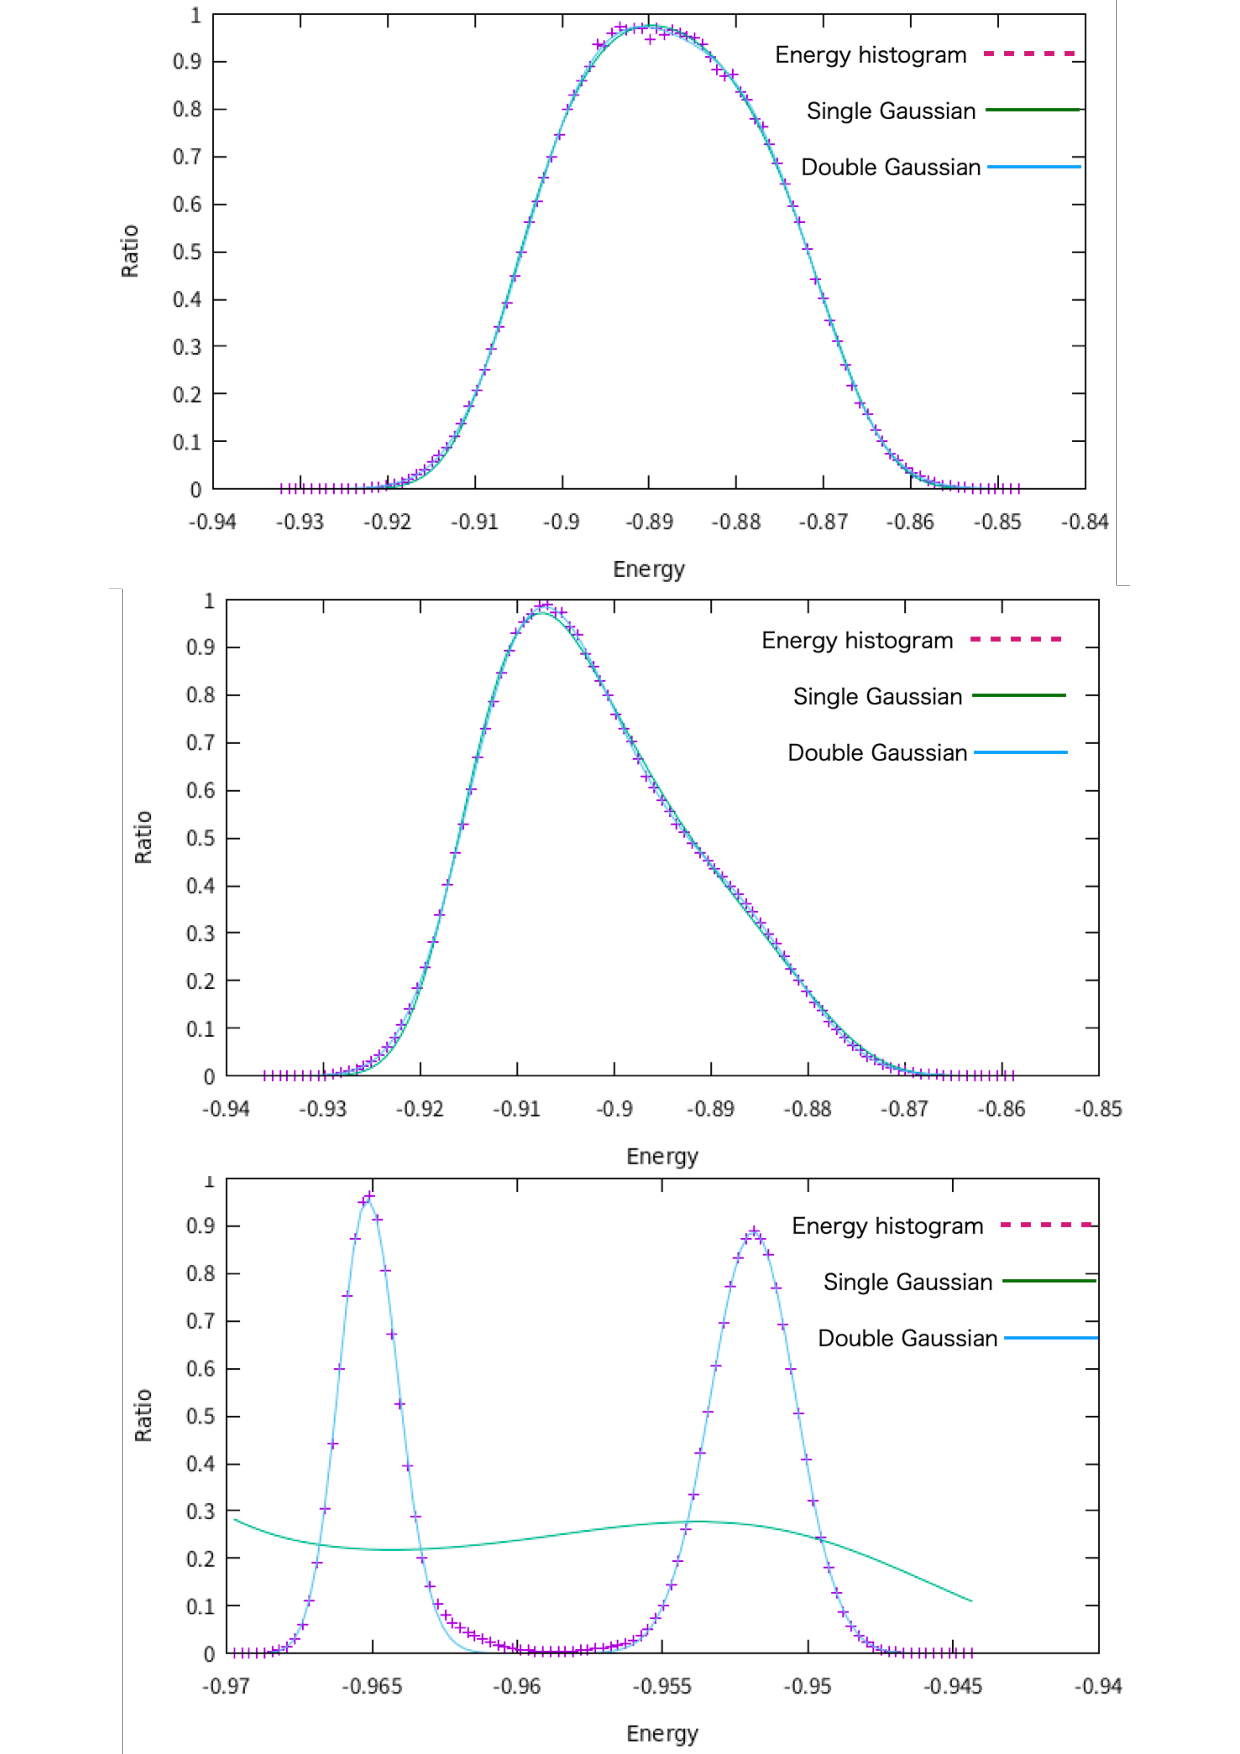
\includegraphics[width=15cm]{figure/energy_histogram.pdf}
%   \caption{代表的な$J_2$でのエネルギーヒストグラム}
%\end{figure}

\newpage

\subsection{秩序変数}
代表的な$J_2$における各秩序変数の温度依存性を示す。
すべて$L=12$の結果である。

まず、$J_2\le0$の場合を議論する。
相図から明らかに$J_2<0$では$m^2_{\sqrt{3}\times\sqrt{3}}$と$\kappa^2_{\mathrm{AFM}}$は値を持たない。
よって、$m^2_{q=0}$と$\kappa^2_{\mathrm{FM}}$と$m^2_{\mathrm{octupole}}$を議論する。
まず、$J_2=0$では、$m^2_{q=0}$と$\kappa^2_{\mathrm{FM}}$のどちらも値を持たない。
一方で、$m^2_{\mathrm{octupole}}$は値を持つため、$J_2=0$における八極子秩序は$q=0$の成分を完全に含まないことがわかる。
次に、$J_2=-5\times10^{-3}$において$m^2_{q=0}$がわずかに値を持つが、$\kappa^2_{\mathrm{FM}}$は値を持たない。
また、比熱に見られた二段転移は存在しない。
これは$J_2=-5\times10^{-3}$における$q=0$相が、カイラリティの長距離秩序を持たない八極子相の性質を受け継いでいることを示唆している。
残りの四点は、以前議論したように、一次転移を示す。
$q=0$秩序と強磁性的カイラリティ秩序と八極子秩序がほぼ同時に転移し、その転移温度は$\abs{J_2}$の増加に伴い上昇する。
%$m^2_{q=0}$と$\kappa^2_{\mathrm{FM}}$と$m^2_{\mathrm{octupole}}$はほぼ同時に転移し、その転移温度は$\abs{J_2}$の増加に伴い上昇する。
%また、相図上で八極子相が存在しない$J_2\ge-2.5\times10^{-2}$においても、$m^2_{\mathrm{octupole}}$が値を持つのは$q=0$秩序が八極子秩序に
\begin{figure}[H]
   \centering
   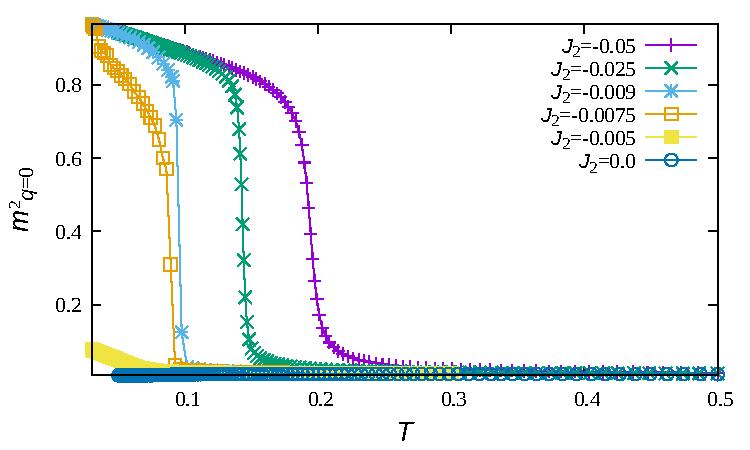
\includegraphics[width=12cm]{figure/mq_q0.pdf}
   \caption{$q=0$磁気秩序変数の温度依存性}
\end{figure}

\begin{figure}[H]
   \centering
   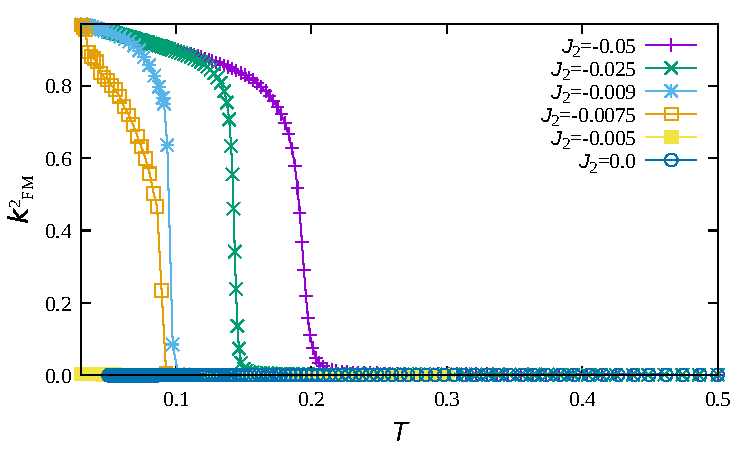
\includegraphics[width=12cm]{figure/fvc.pdf}
   \caption{強磁性的カイラリティ秩序変数の温度依存性}
\end{figure}

次に、$J_2\ge0$を議論する。
$J2\le0$と同様の事情で、$\sqrt{3}\times\sqrt{3}$秩序と反強磁性的カイラリティ秩序と八極子秩序の秩序変数のみを議論する。
基本的な性質は$J_2\le0$と同様である。
すなわち、$\sqrt{3}\times\sqrt{3}$秩序と反強磁性的カイラリティ秩序がほぼ同時に転移し、その転移温度は$\abs{J_2}$の増加に伴い上昇する。
一方で、各秩序変数が$J2\le0$の一次転移領域の秩序変数よりも緩やかに変化する点、$J_2=0$で$m^2_{\sqrt{3}\times\sqrt{3}}$が有限である点で$J_2\le0$と異なる。
前者は、$J_2\ge0$が連続転移であることから説明できる。
一般に、一次転移における転移温度での秩序変数の変化は、連続転移の場合よりも激しい。
後者を整理すると、$J_2=0$において、$m^2_{\sqrt{3}\times\sqrt{3}}$と$m^2_{\mathrm{octupole}}$が有限で、$\kappa^2_{\mathrm{AFM}}$のみ有限ではない。
この結果と$J_2=0$において$m^2_{q=0}$と$\kappa^2_{\mathrm{FM}}$が有限ではないという結果から、以下のことがわかる。
すなわち、$J_2=0$における八極子秩序は確かにカイラリティの長距離秩序を示さず、かつ$q=0$より$\sqrt{3}\times\sqrt{3}$に似た磁気秩序を示す。
%これは、$J_2=0$における非平衡緩和法の初期状態として$q=0$状態ではなく$\sqrt{3}\times\sqrt{3}$状態を選んだ根拠となった。


\begin{figure}[H]
   \centering
   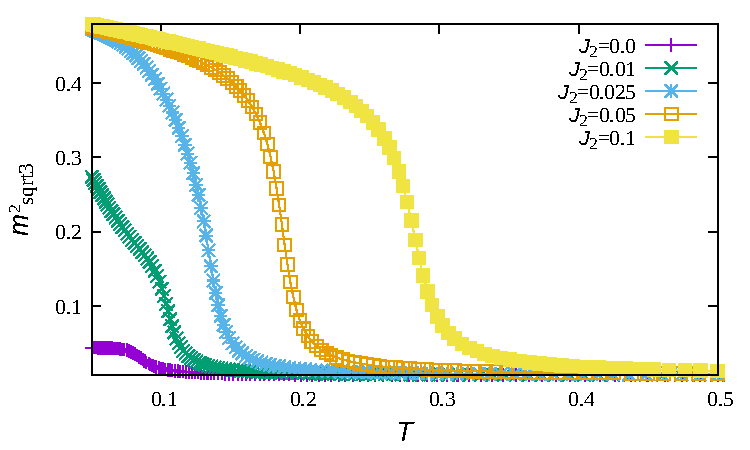
\includegraphics[width=12cm]{figure/mq_sqrt3.pdf}
   \caption{$\sqrt{3}\times\sqrt{3}$磁気秩序変数の温度依存性}
\end{figure}

\begin{figure}[H]
   \centering
   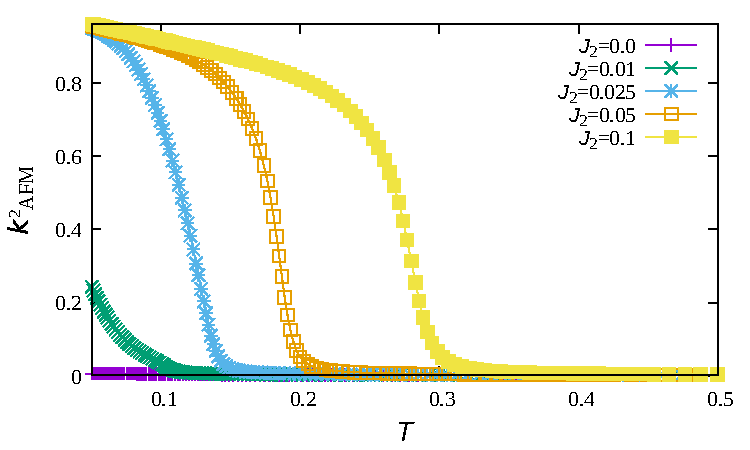
\includegraphics[width=12cm]{figure/afvc.pdf}
   \caption{反強磁性的カイラリティ秩序変数の温度依存性}
\end{figure}

\begin{figure}[H]
   \centering
   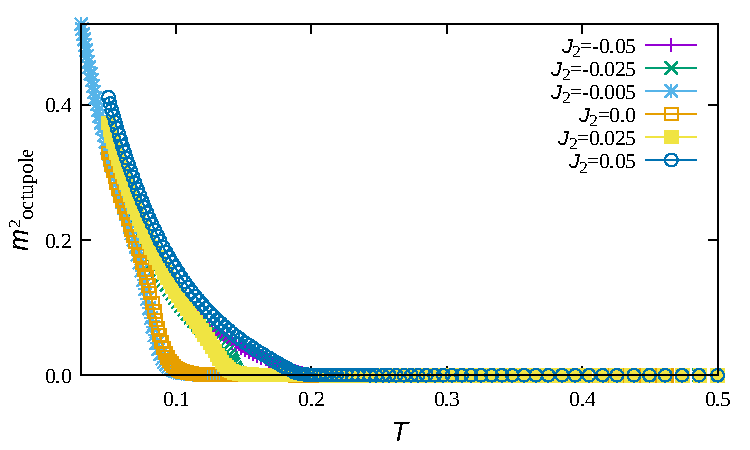
\includegraphics[width=12cm]{figure/octupole.pdf}
   \caption{八極子秩序変数の温度依存性}
\end{figure}

%\begin{figure}[H]
%   \centering
%   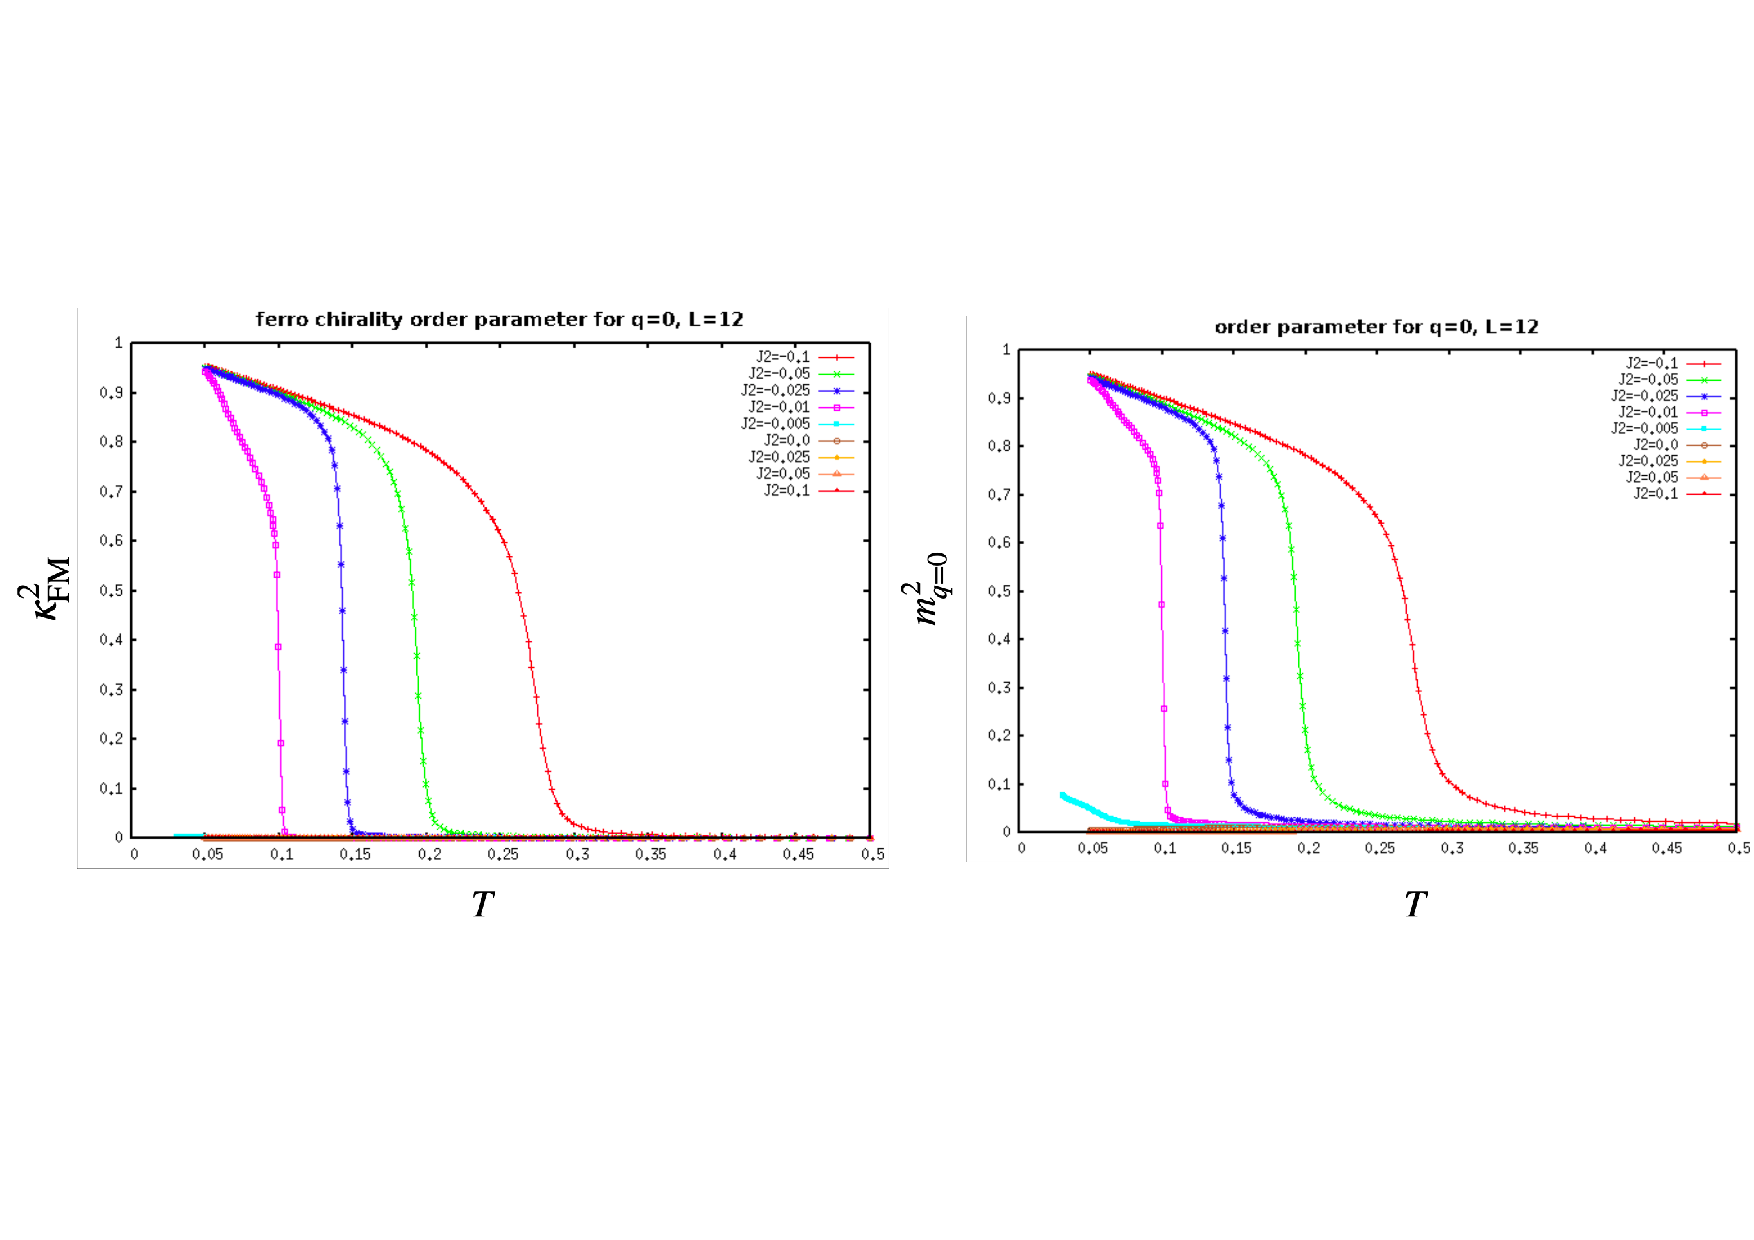
\includegraphics[width=15cm]{figure/order_params_q0.pdf}
%   \caption{強磁性的カイラリティ秩序変数と$q=0$磁気秩序変数の温度依存性}
%\end{figure}
%
%\begin{figure}[H]
%   \centering
%   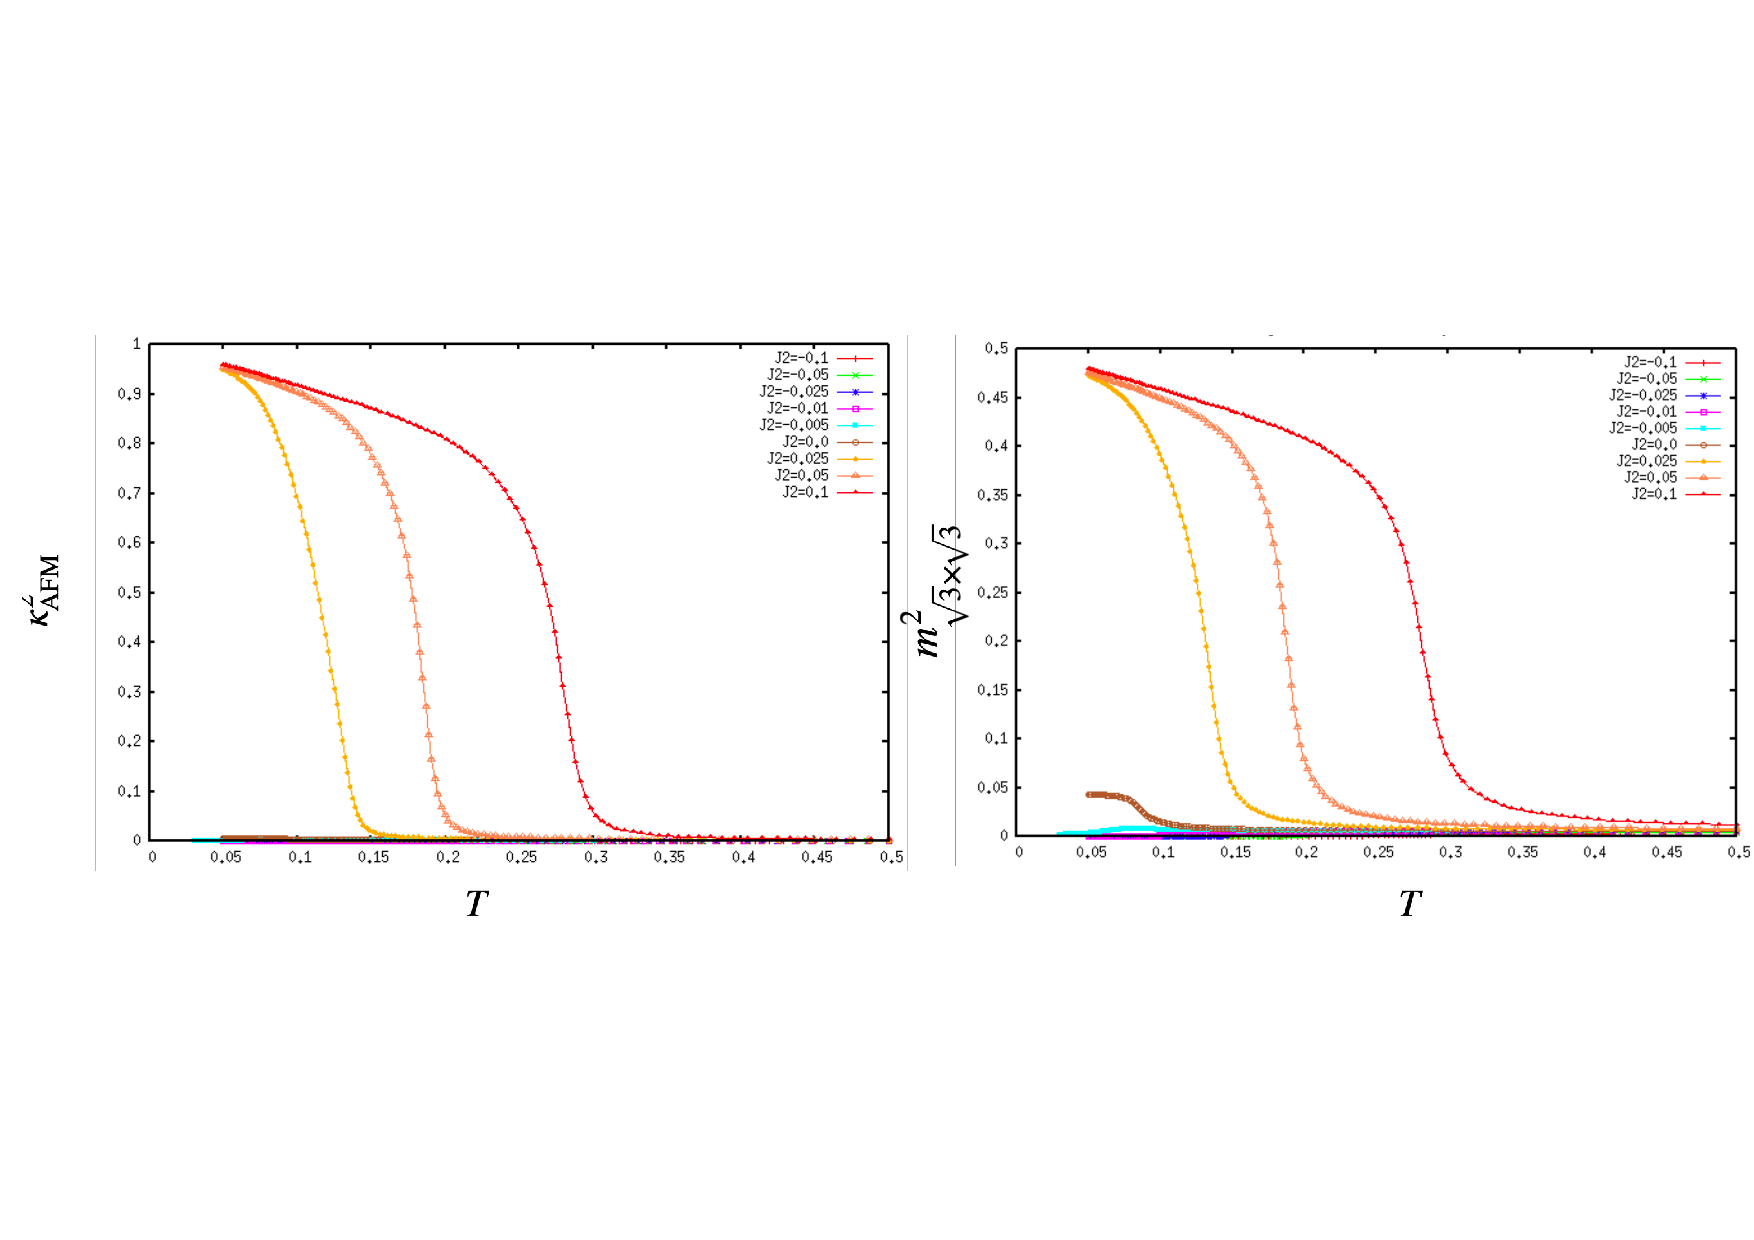
\includegraphics[width=15cm]{figure/order_params_sqrt3.pdf}
%   \caption{反強磁性的カイラリティ秩序変数と$\sqrt{3}\times\sqrt{3}$磁気秩序変数の温度依存性}
%\end{figure}

%\begin{figure}[H]
%   \centering
%   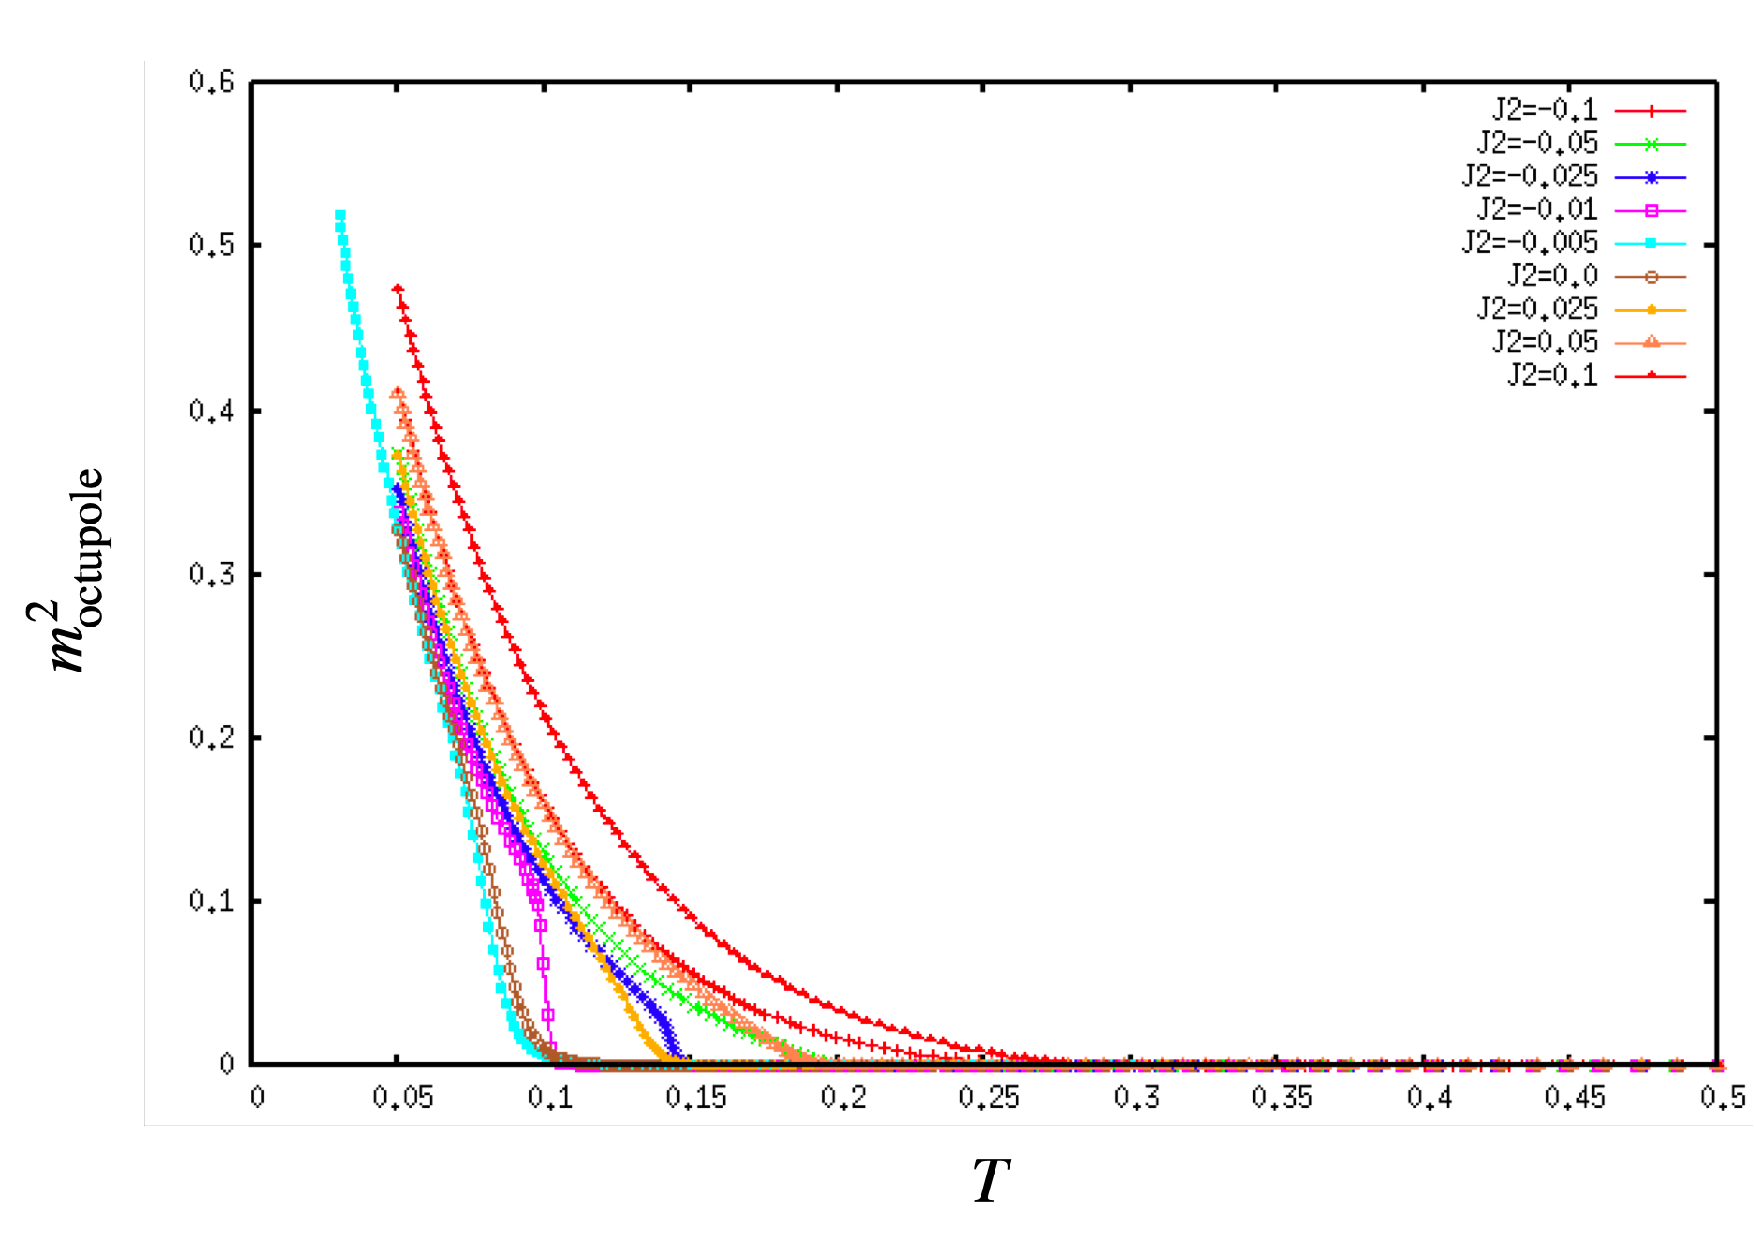
\includegraphics[width=12cm]{figure/octupole_order_params.pdf}
%   \caption{八極子秩序変数の温度依存性}
%\end{figure}

\newpage

\subsection{各秩序変数の緩和過程と緩和時間}
ここからは、非平衡緩和法の結果を議論する。
各$J_2$において、それぞれの秩序変数の緩和過程と緩和時間の温度依存性を示した。

一般に、一次転移近傍では非平衡緩和法を行うことは難しい。
本研究では$J_2=0$と$J_2=-2.5\times10^{-3}$がこれに当たる。
そこで、まずこの二点にについて議論する。
また、この二点では、モンテカルロ更新の凍結により、磁気秩序のBKT転移とカイラリイティ転移の転移温度の推定できていない。
よって、八極子秩序のBKT転移のみ議論する。
一次転移に近いことを考慮して、十分な精度を出すために$J_2=0$では240サンプル、$J_2=-2.5\times10^{-3}$では210サンプルの平均を取った。
また、どちらも$L=1800$で計算した。
$J_2=0$の緩和過程は$T=0.08$で系が臨界的になっていることを示唆している。
また、40サンプルごとに分割し、それぞれ独立に転移温度を計算し統計処理を行った。
その結果、転移温度は
\begin{align}
   T_{\mathrm{octupole}}= 0.067 \pm 0.002
\end{align}
となった。
非平衡緩和法は$T>T_{\mathrm{BKT}}$のデータからの外挿によって転移温度を推定する。
そのため、計算結果は緩和過程から推定される温度よりも低くなることが多い。
これによって$T_{\mathrm{octupole}}<0.08$を説明できる。
また、$T_{\mathrm{octupole}}$は過去の結果$T_{\mathrm{octupole}}'=0.070\sim0.076$\cite{Rzchowski1997}の下限にほぼ一致する。
緩和時間の温度依存性は240サンプルすべてを使って計算した。
これを見ると、240サンプル取ることで$G_{\mathrm{octupole}}$のゆらぎを抑制して尚、緩和時間は低温でなめらかにならない。
40サンプルに分割したとき、この問題がより顕著になり、$T_{\mathrm{octupole}}$の誤差の要因となっていると考えられる。
次に、$J_2=-2.5\times10^{-3}$の結果を示す。
前述のように210サンプル取った。
$J_2=0$と同じく、緩和過程は$T=0.078$で既に臨界的になっていることを示唆しているが、転移温度は
\begin{align}
   T_{\mathrm{octupole}} = 0.065 \pm 0.005
\end{align}
となった。
$J_2=0$の結果に比べ標準偏差が増加しているが、これは$J_2=-2.5\times10^{-3}$が$J_2=0$よりも一次転移領域に近く、非平衡緩和法が不安定になることを反映していると考えられる。
また、$J_2=-2.5\times10^{-3}$において八極子相が存在し、BKT転移温度が$J_2=0$と異なるという結果は、八極子相が$-10^{-3}<J_2/J_1<10^{-4}$に存在し、BKT転移温度は$J_2/J_1$に依存せず一定であるという先行研究の主張に矛盾する。

%\begin{align}
%   T_{\mathrm{octupole}} = 0.0653701 \pm 0.004987432522350554
%\end{align}
%誤差の要因として以下、二点が考えられる。
%一つ目は、それぞれの転移温度はわずか40サンプルのデータから計算されているため、サンプルごとのゆらぎを完全に抑制できていない点。
%二つ目は、先行研究の転移温度が平衡法によって決められているため、有限サイズ効果が混入している点。

%\begin{align}
%   T_{\mathrm{octupole}}= 0.06723238333333333 \pm 0.0015808125814487516
%\end{align}

%\begin{itemize}
%   \item ここからは、非平衡緩和法の結果を議論する。
%   \item 下に各$J_2$におけるそれぞれの秩序変数の緩和過程と緩和時間温度依存性を示す。
%   \item 一次転移に近い$J_2=-2.5\times10^{-3}$と$J_2=0$ではそれぞれ210サンプル、
%\end{itemize}
\begin{figure}[H]
   \centering
   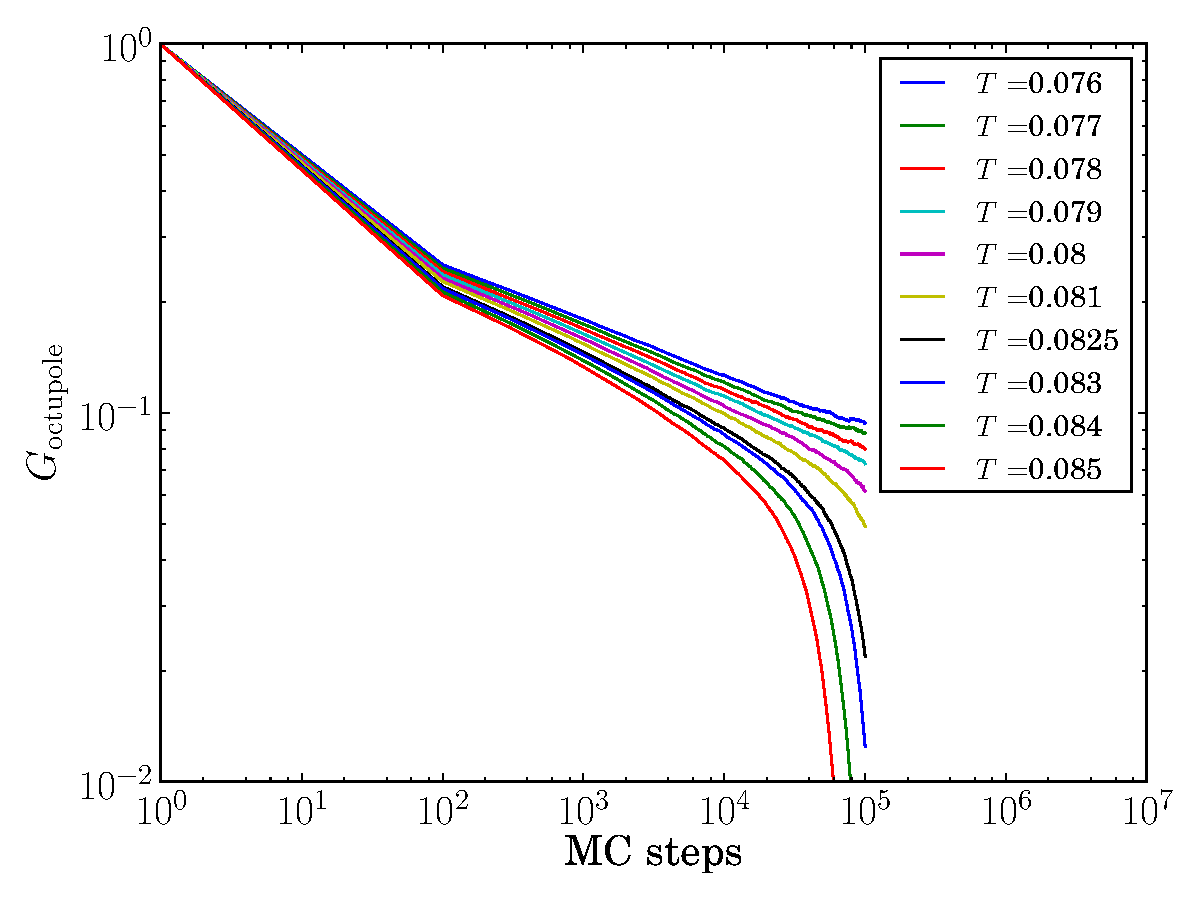
\includegraphics[width=12cm]{figure/octupole_raw_data_j2_0.pdf}
   \caption{$J_2=0$の八極子秩序変数の緩和過程}
\end{figure}

\begin{figure}[H]
   \centering
   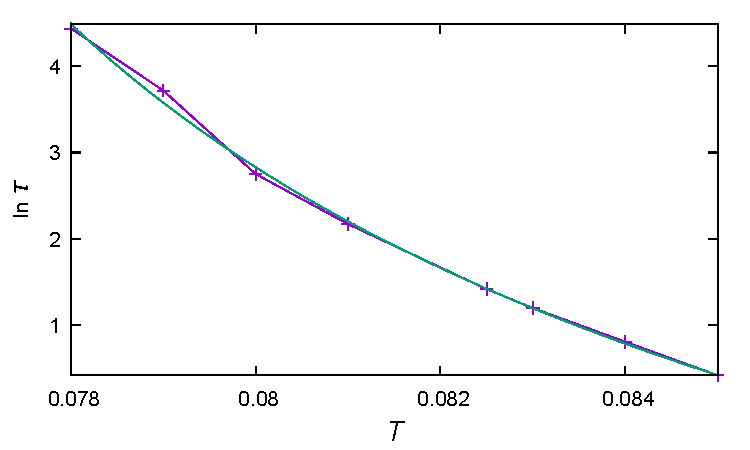
\includegraphics[width=12cm]{figure/octupole_Tc_j2_0.pdf}
   \caption{$J_2=0$の八極子秩序変数の緩和時間の温度依存性}
\end{figure}

\begin{figure}[H]
   \centering
   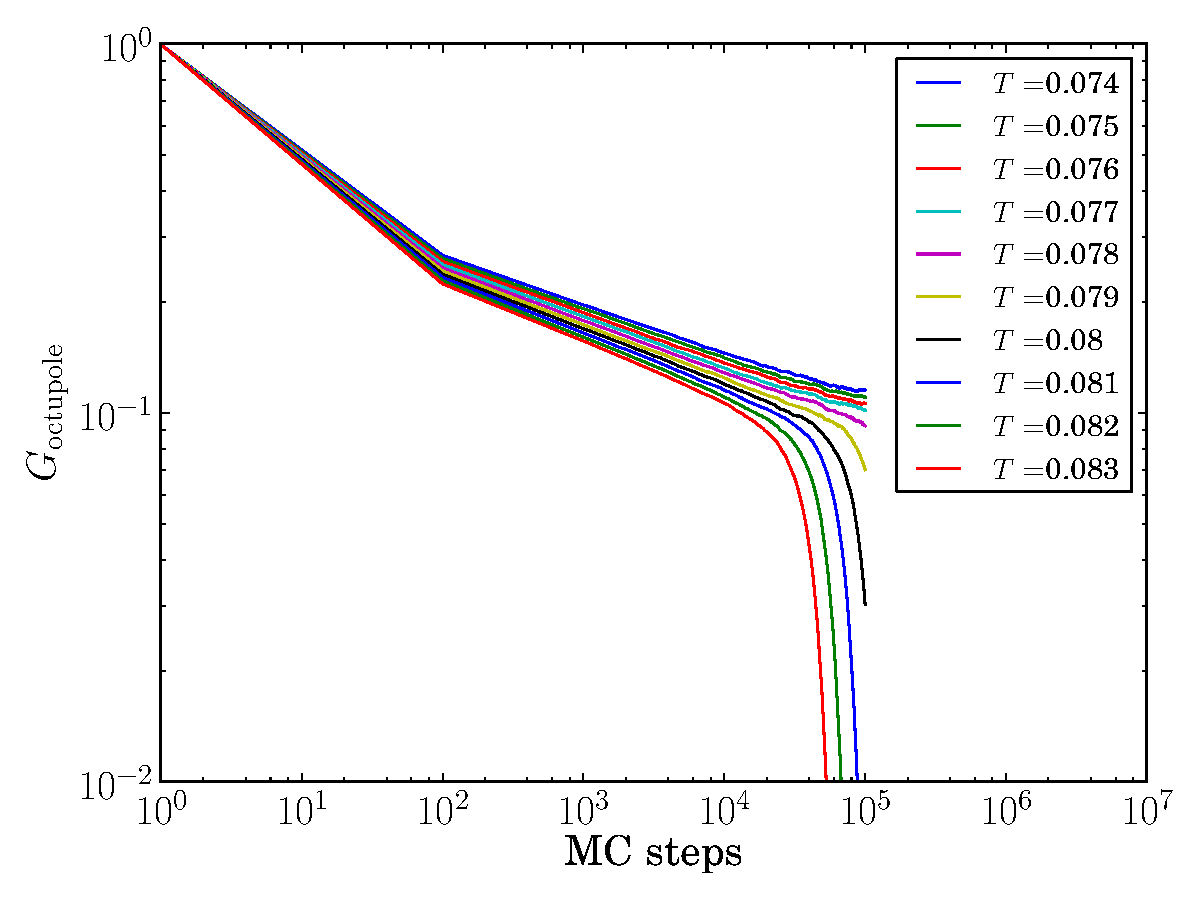
\includegraphics[width=12cm]{figure/octupole_raw_data_j2_-2.5e-3.pdf}
   \caption{$J_2=-0.0025$の八極子秩序変数の緩和過程}
\end{figure}

\begin{figure}[H]
   \centering
   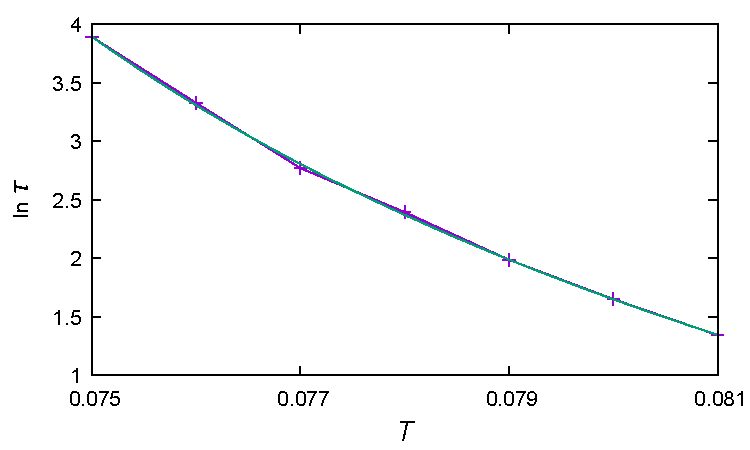
\includegraphics[width=12cm]{figure/octupole_Tc_j2_-2.5e-3.pdf}
   \caption{$J_2=-0.0025$の八極子秩序変数の緩和時間の温度依存性}
\end{figure}

%\begin{figure}[H]
%   \centering
%   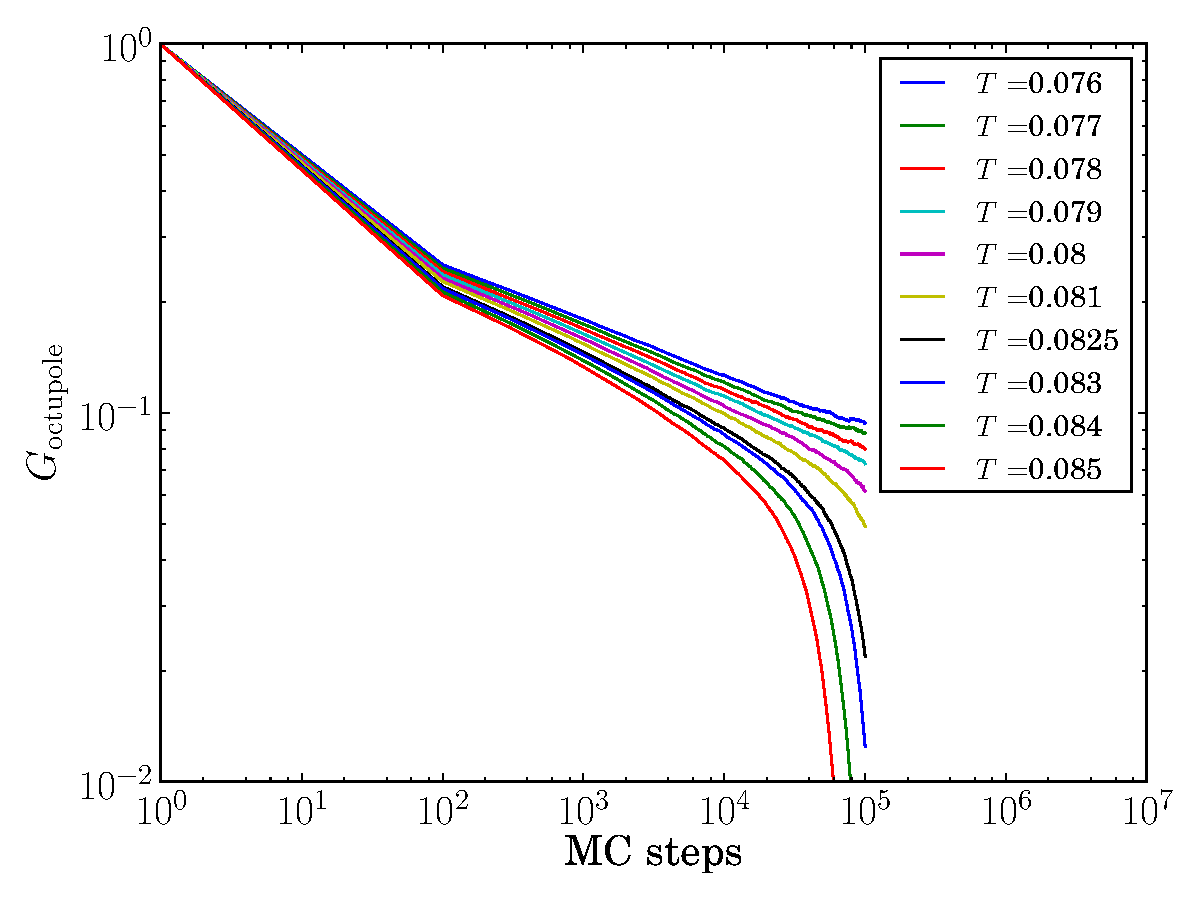
\includegraphics[width=12cm]{figure/octupole_raw_data_j2_0.pdf}
%   \caption{$J_2=0$の八極子秩序変数の緩和過程}
%\end{figure}
%
%\begin{figure}[H]
%   \centering
%   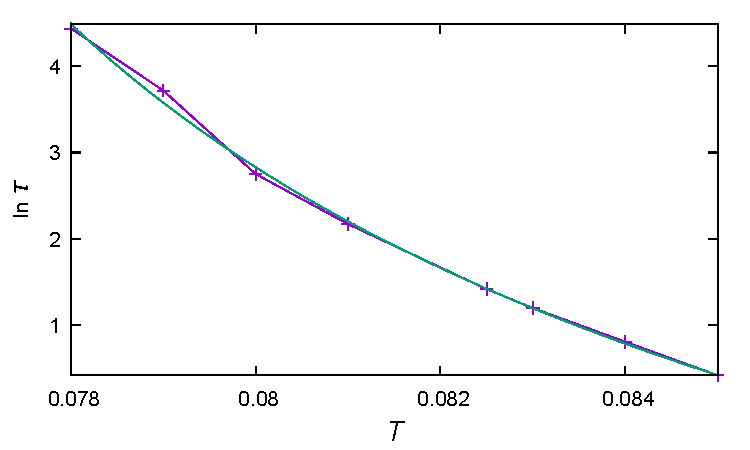
\includegraphics[width=12cm]{figure/octupole_Tc_j2_0.pdf}
%   \caption{$J_2=0$の八極子秩序変数の緩和時間の温度依存性}
%\end{figure}

\newpage

最後に、$J_2>0$の結果を紹介する。
この領域は一次転移領域から十分離れているため、少ないサンプル数で計算した。

まず、$J_2=-1\times10^{-2}$について議論する。
$L=900$、5サンプルの計算を行った。
各秩序変数の転移温度は
\begin{align}
   T_{\sqrt{3}\times\sqrt{3}} &= 0.059 \pm 0.016, \\ 
   T_{\mathrm{AFM}}           &= 0.058 \pm 0.011, \\
   T_{\mathrm{octupole}}      &= 0.092 \pm 0.003. 
\end{align}
$J_2=-1\times10^{-2}$では$T_{\sqrt{3}\times\sqrt{3}},T_{\mathrm{AFM}}$と$T_{\mathrm{octupole}}$が明らかに分離している。
また、低温でのエラーが大きいため、$T_{\sqrt{3}\times\sqrt{3}}$と$T_{\mathrm{AFM}}$の大小関係は判然としない。

%\begin{align}
%   T_{\sqrt{3}\times\sqrt{3}} &= 0.059 \pm 0.016 (27.41\%), \\ 
%   T_{\mathrm{AFM}}           &= 0.058 \pm 0.011 (18.92\%), \\
%   T_{\mathrm{octupole}}      &= 0.092 \pm 0.003 (3.028\%). 
%\end{align}

次に、$J_2=-2\times10^{-2}$について議論する。
$L=1800$、10サンプルの計算を行った。
各秩序変数の転移温度は
\begin{align}
   T_{\sqrt{3}\times\sqrt{3}} &= 0.106 \pm 0.001, \\
   T_{\mathrm{AFM}}           &= 0.107 \pm 0.001, \\
   T_{\mathrm{octupole}}      &= 0.100 \pm 0.004. 
\end{align}
$J_2=-2\times10^{-2}$では、誤差を考慮すれば、三つの秩序がほぼ同時に転移する。
また、$T_{\sqrt{3}\times\sqrt{3}}$と$T_{\mathrm{AFM}}$の間に$10^{-3}$のオーダーの分離が見られる($T_{\mathrm{AFM}}>T_{\sqrt{3}\times\sqrt{3}}$)。
これは、過去に行われた幾何学的フラストレート磁性体に対する非平衡緩和法の結果\cite{Misawa2010}と整合する。

%\begin{align}
%   T_{\sqrt{3}\times\sqrt{3}} &= 0.106 \pm 0.001(0.6071\%), \\
%   T_{\mathrm{AFM}}           &= 0.107 \pm 0.001(0.8501\%), \\
%   T_{\mathrm{octupole}}      &= 0.100 \pm 0.004(4.018 \%). 
%\end{align}
\begin{figure}[H]
   \centering
   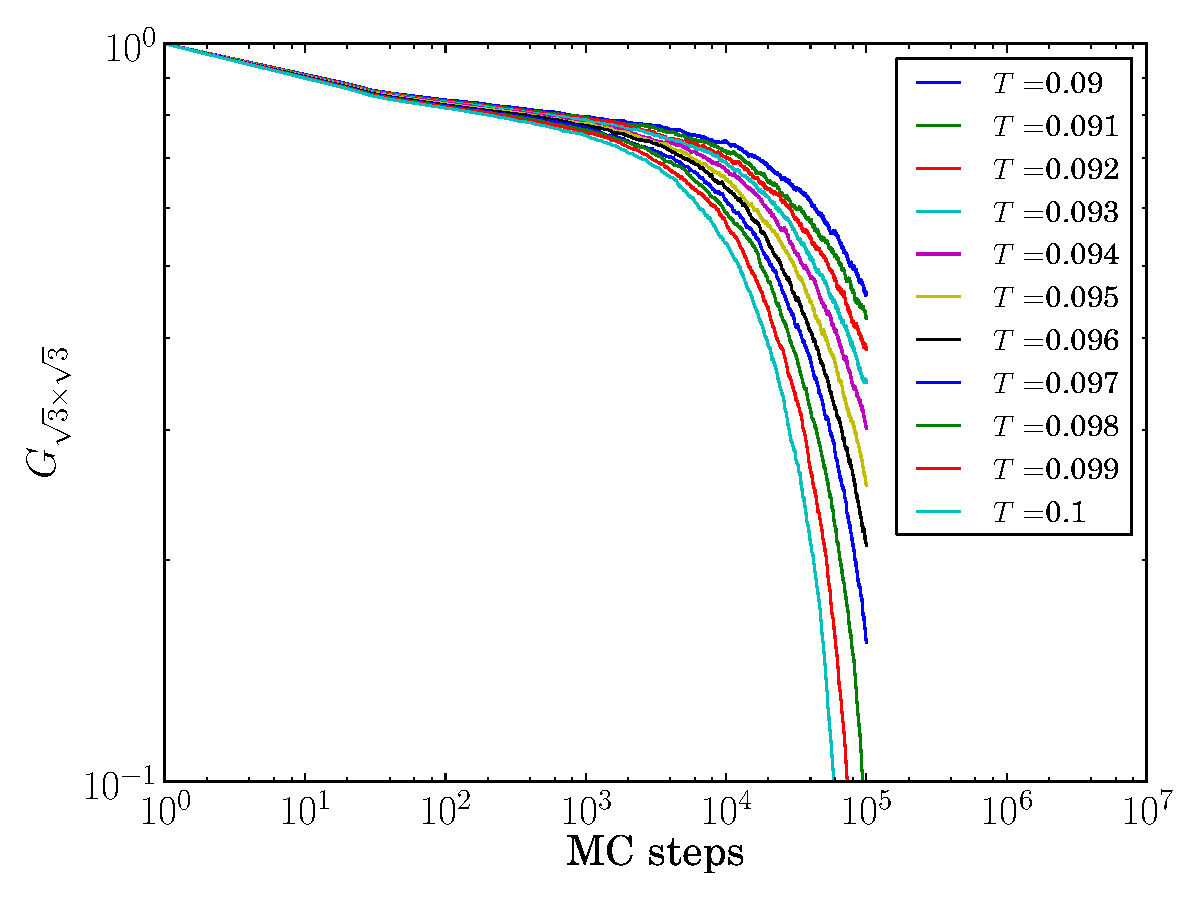
\includegraphics[width=12cm]{figure/mq_sqrt3_raw_data_j2_0.01.pdf}
   \caption{$J_2=0.01$の$\sqrt{3}\times\sqrt{3}$磁気秩序変数の緩和過程}
\end{figure}

\begin{figure}[H]
   \centering
   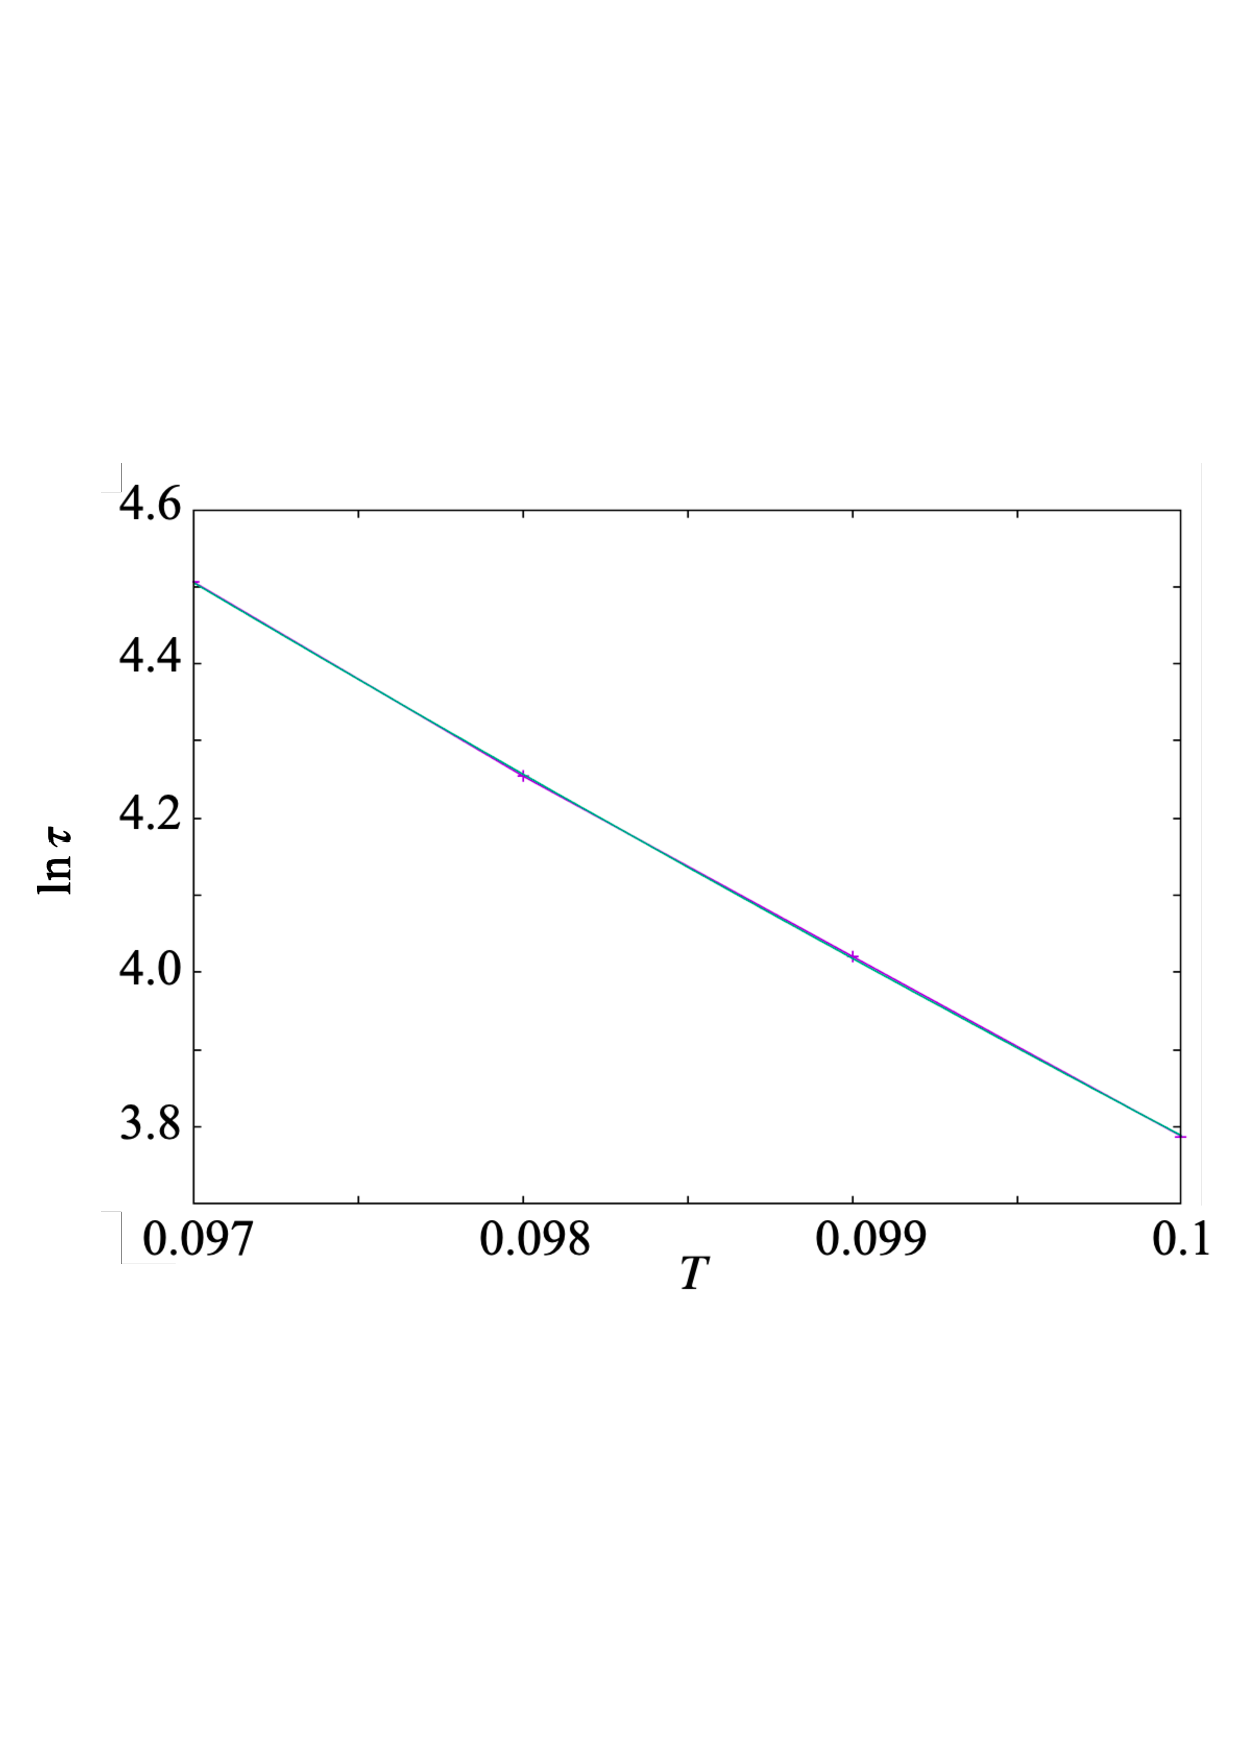
\includegraphics[width=12cm]{figure/mq_sqrt3_Tc_j2_0.01.pdf}
   \caption{$J_2=0.01$の$\sqrt{3}\times\sqrt{3}$磁気秩序変数の緩和時間の温度依存性}
\end{figure}

\begin{figure}[H]
   \centering
   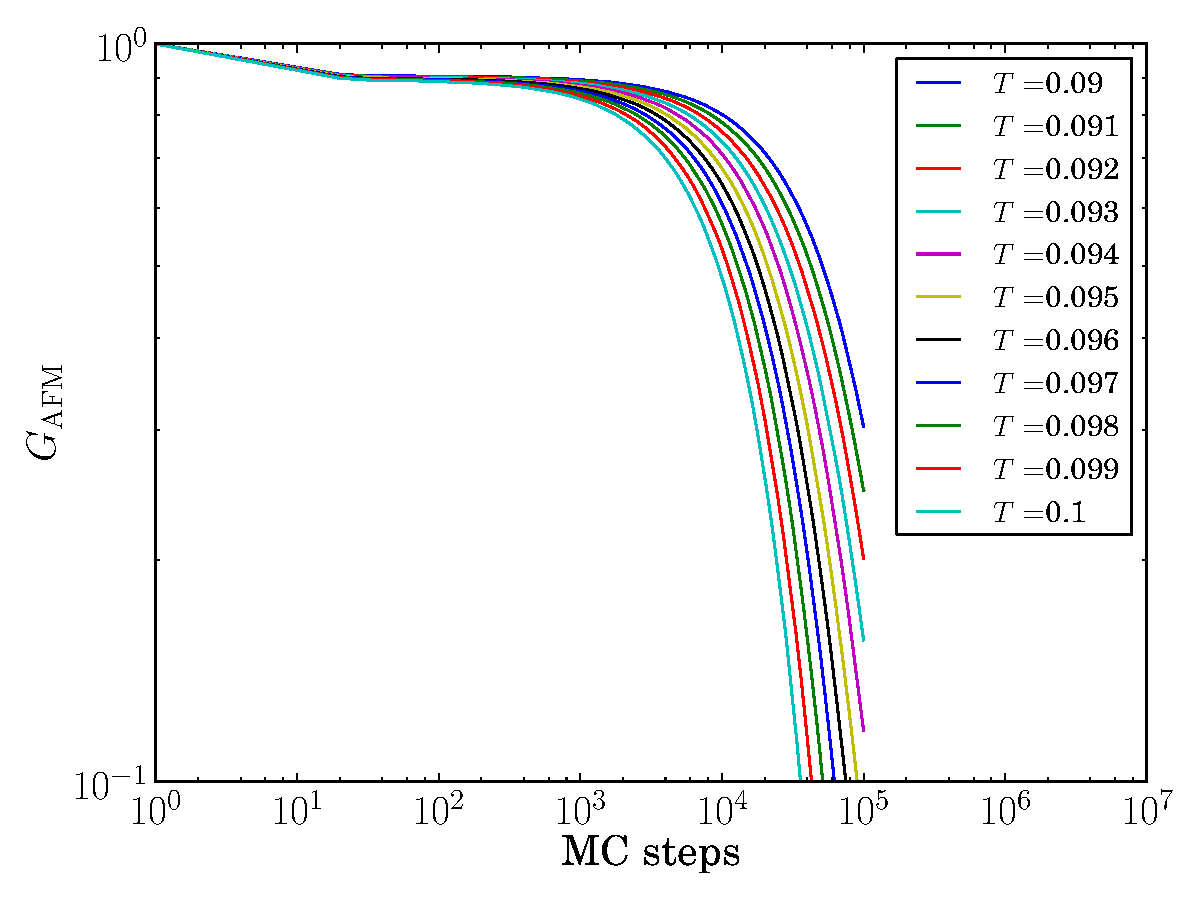
\includegraphics[width=12cm]{figure/afvc_raw_data_j2_0.01.pdf}
   \caption{$J_2=0.01$の反強磁性カイラリティ秩序変数の緩和過程}
\end{figure}

\begin{figure}[H]
   \centering
   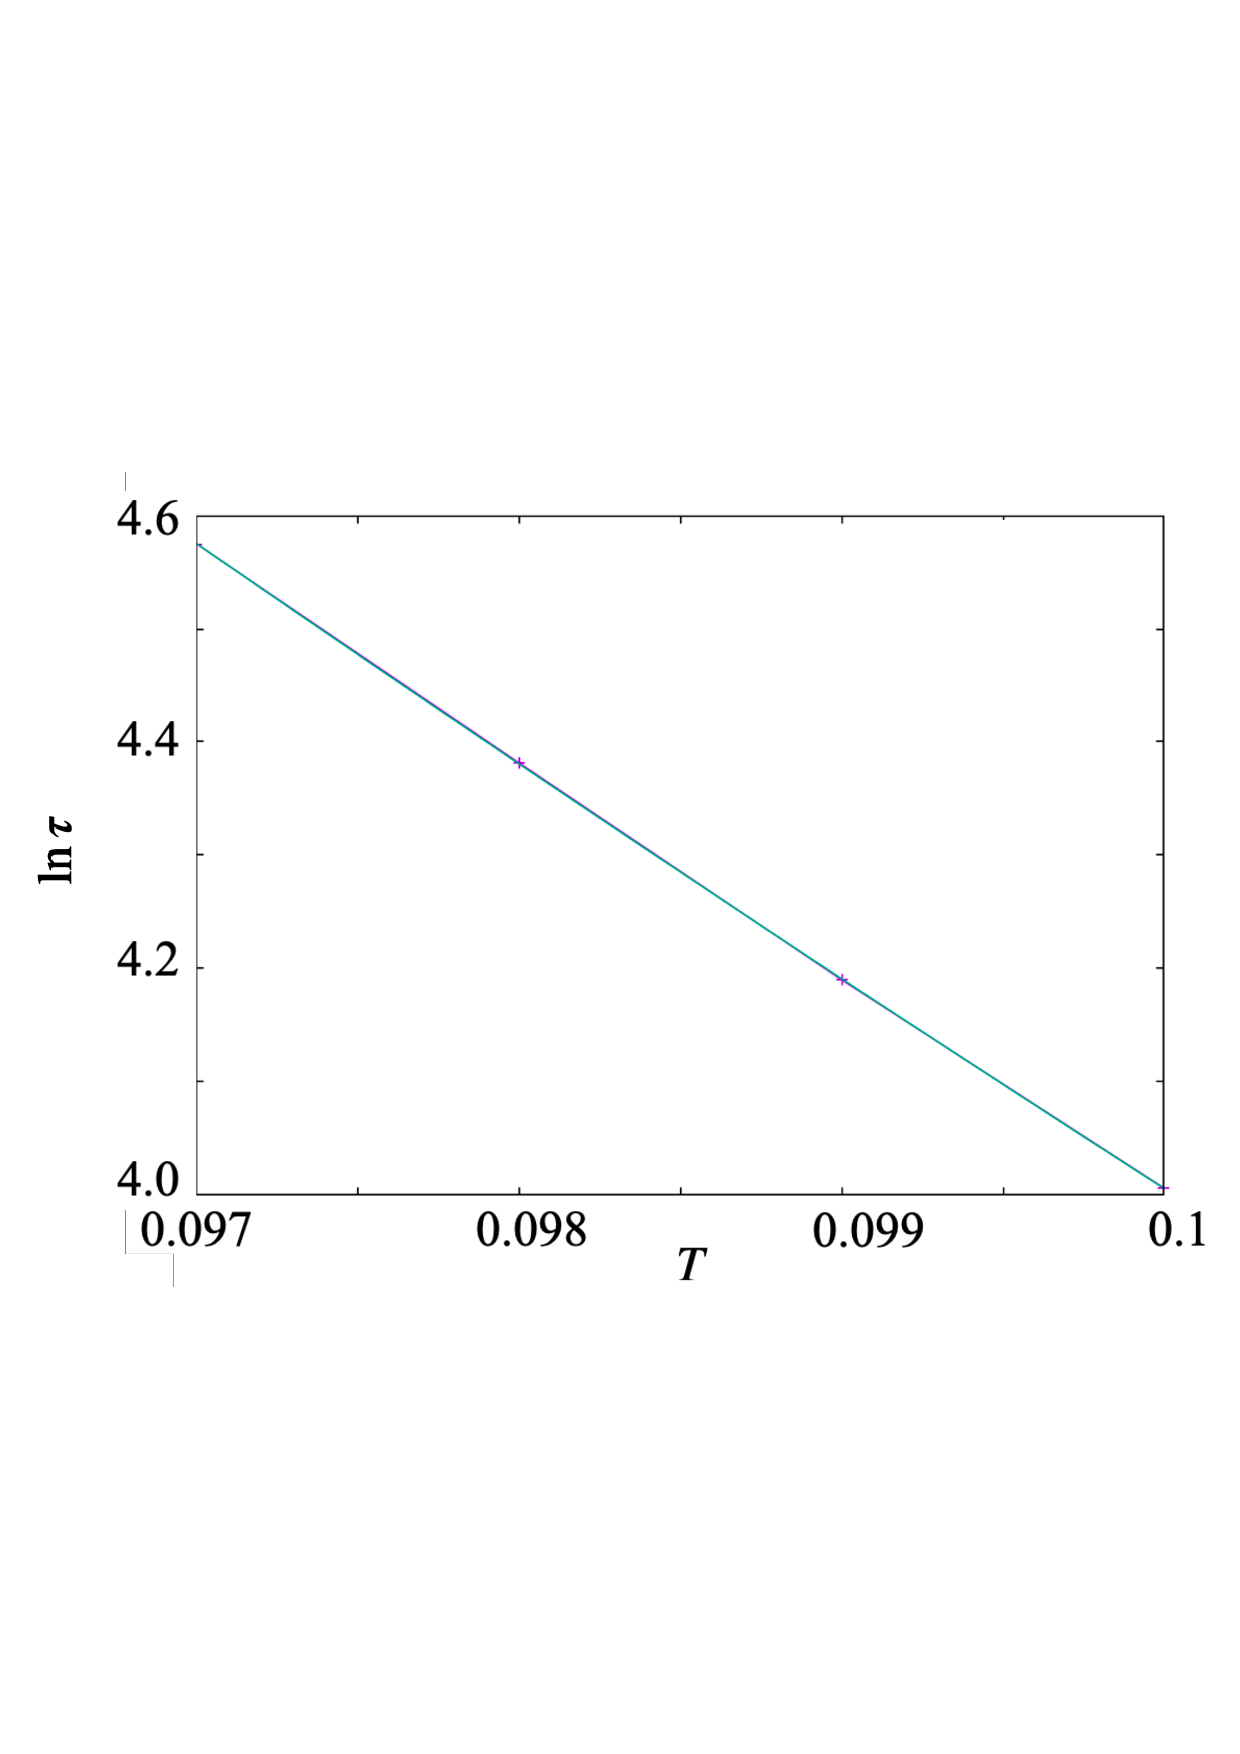
\includegraphics[width=12cm]{figure/afvc_Tc_j2_0.01.pdf}
   \caption{$J_2=0.01$の反強磁性カイラリティ秩序変数の緩和時間の温度依存性}
\end{figure}

\begin{figure}[H]
   \centering
   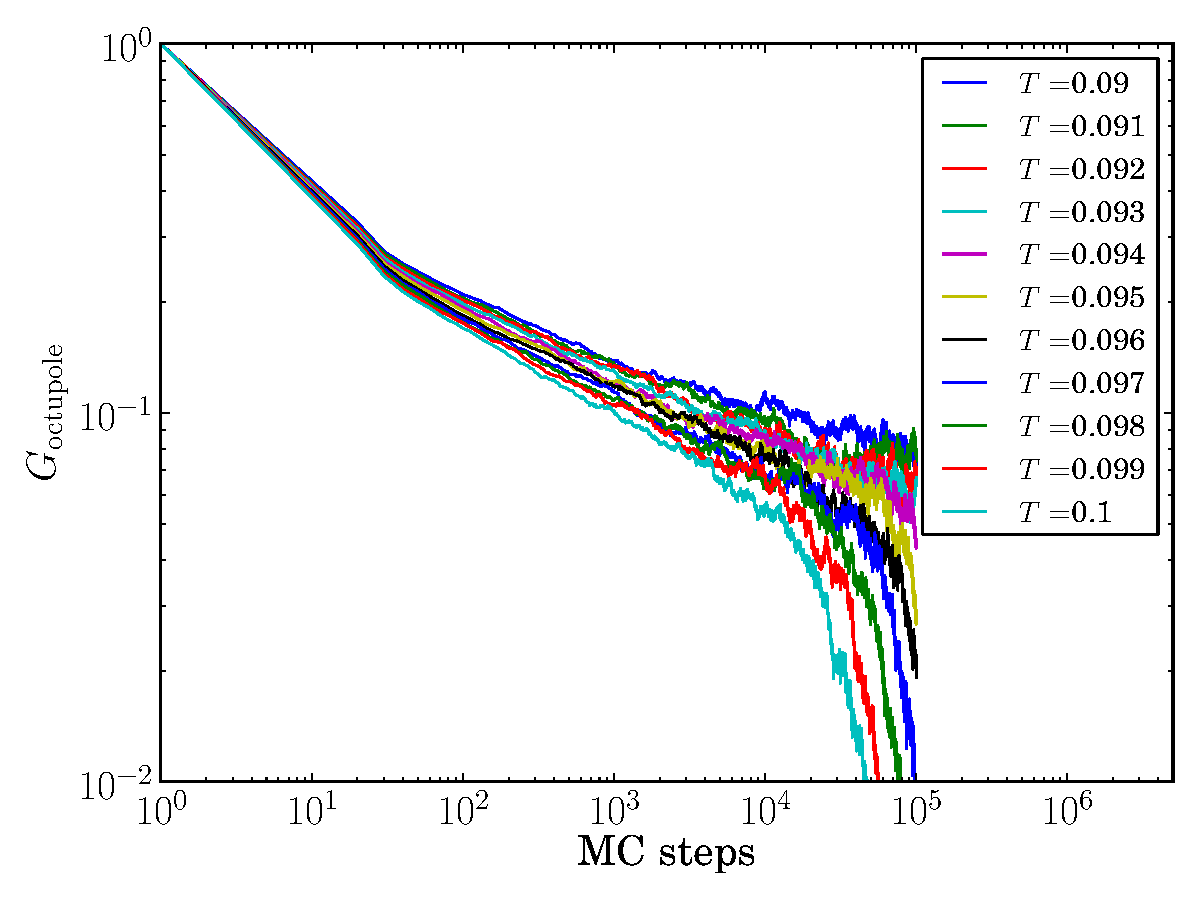
\includegraphics[width=12cm]{figure/octupole_raw_data_j2_0.01.pdf}
   \caption{$J_2=0.01$の八極子秩序変数の緩和過程}
\end{figure}

\begin{figure}[H]
   \centering
   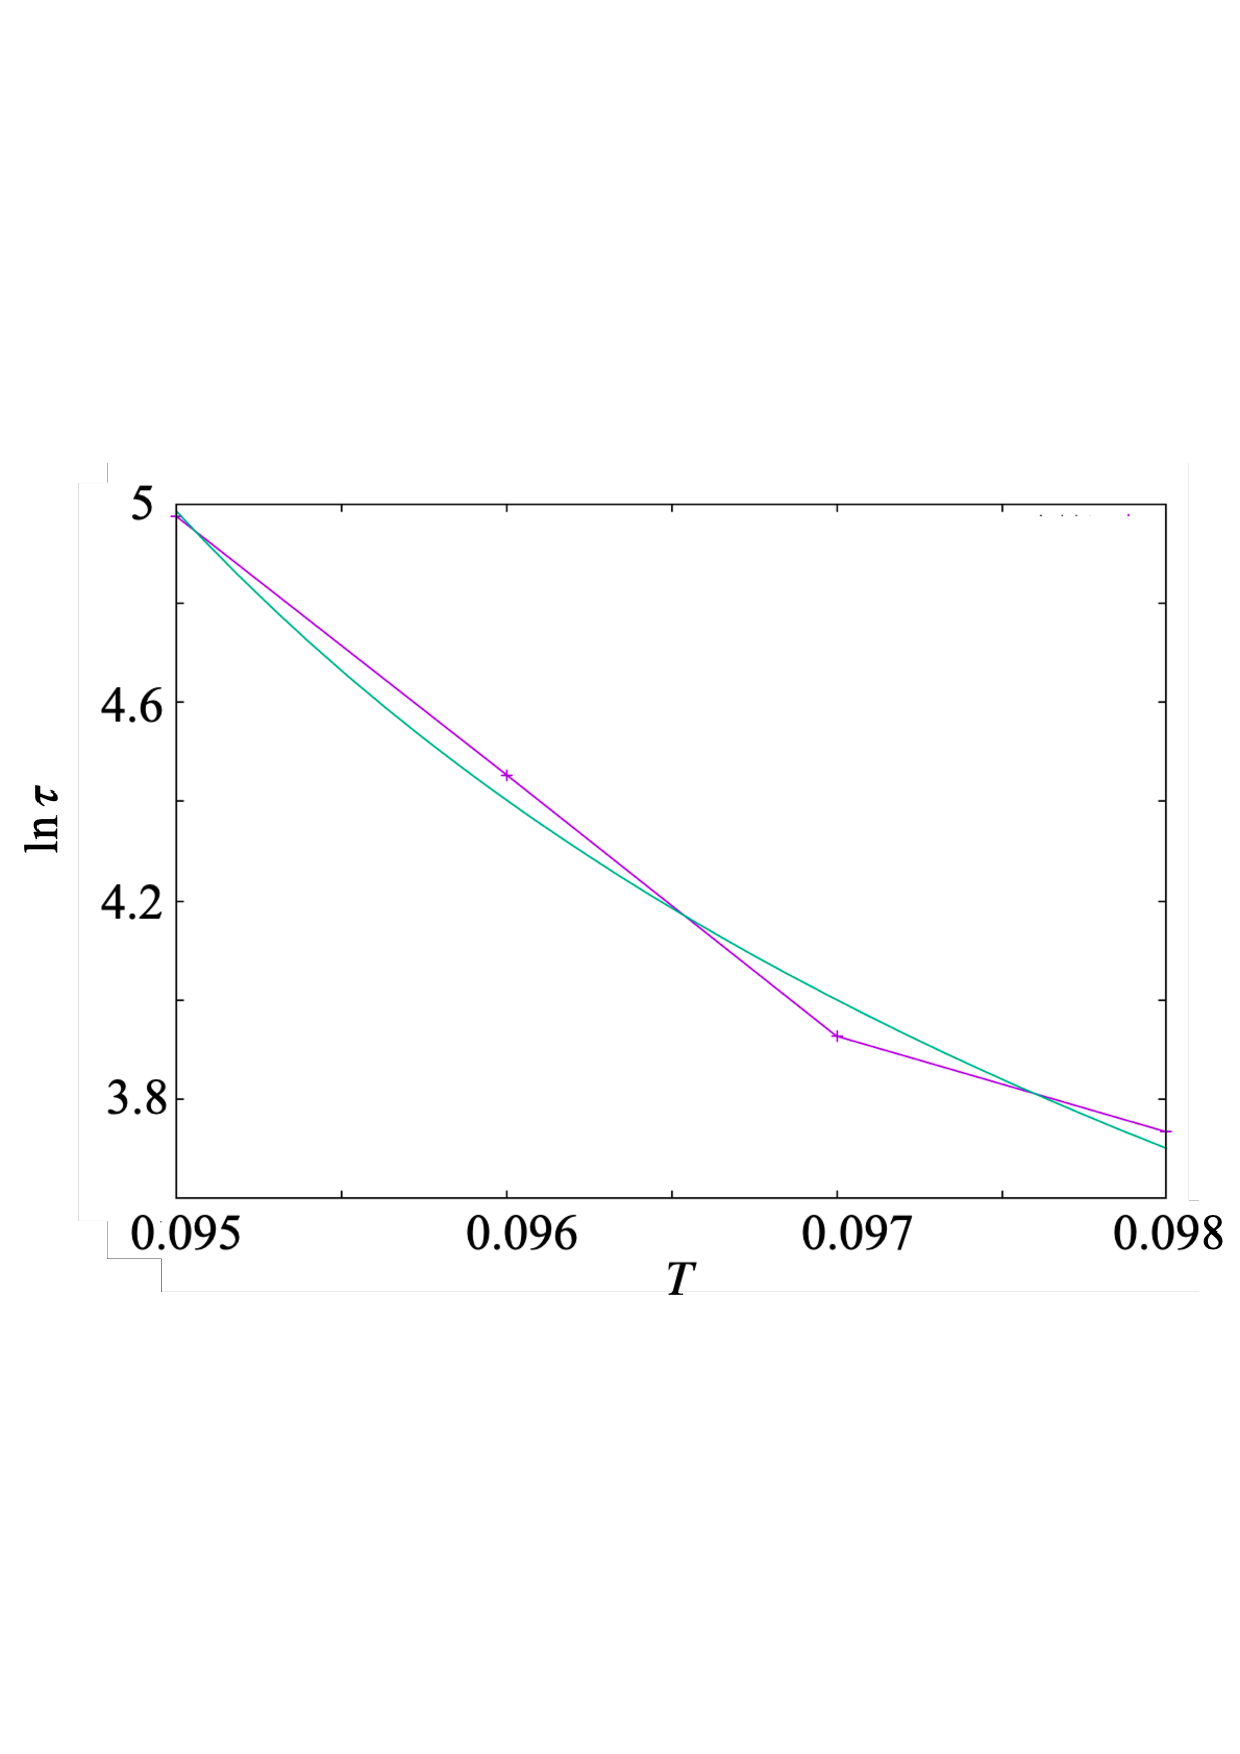
\includegraphics[width=12cm]{figure/octupole_Tc_j2_0.01.pdf}
   \caption{$J_2=0.01$の八極子秩序変数の緩和時間の温度依存性}
\end{figure}

\begin{figure}[H]
   \centering
   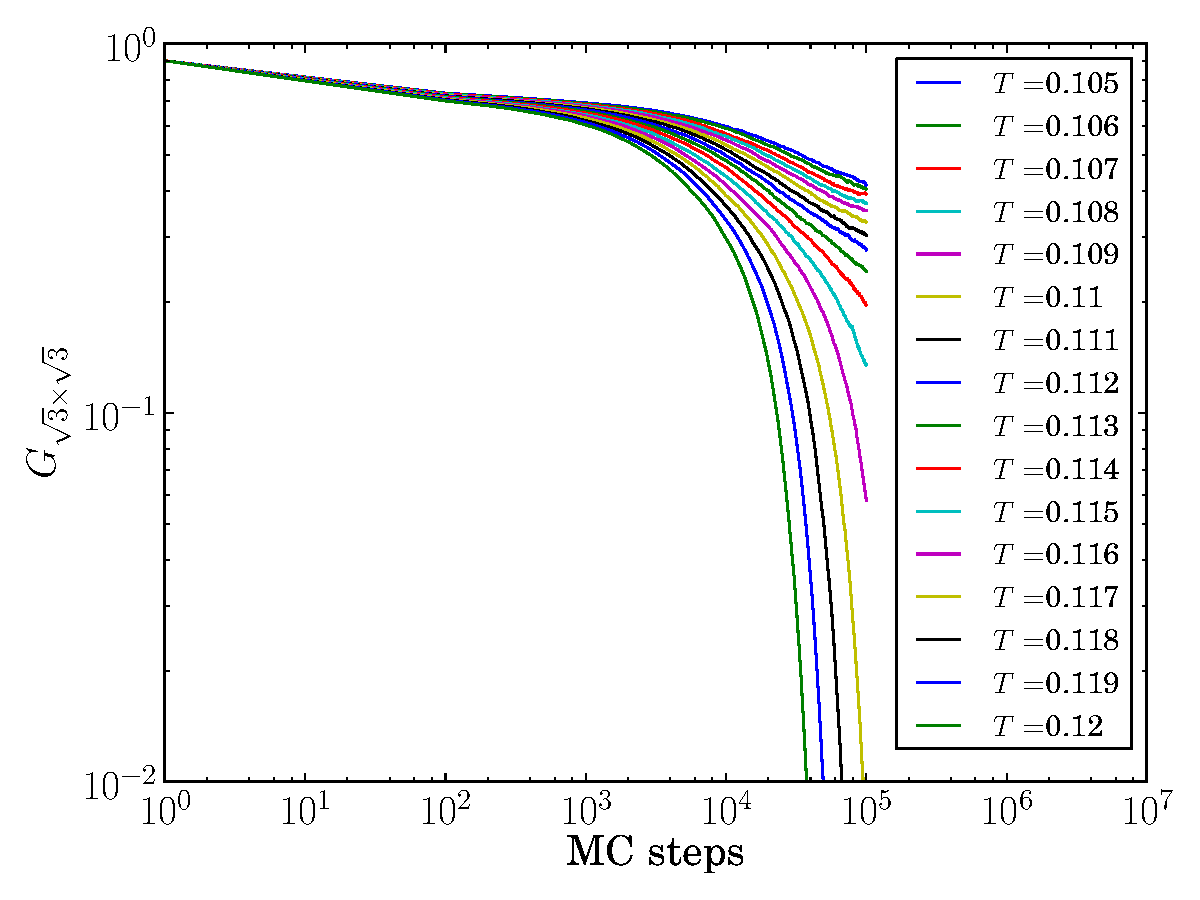
\includegraphics[width=12cm]{figure/mq_sqrt3_raw_data_j2_0.02.pdf}
   \caption{$J_2=0.02$の$\sqrt{3}\times\sqrt{3}$磁気秩序変数の緩和過程}
\end{figure}

\begin{figure}[H]
   \centering
   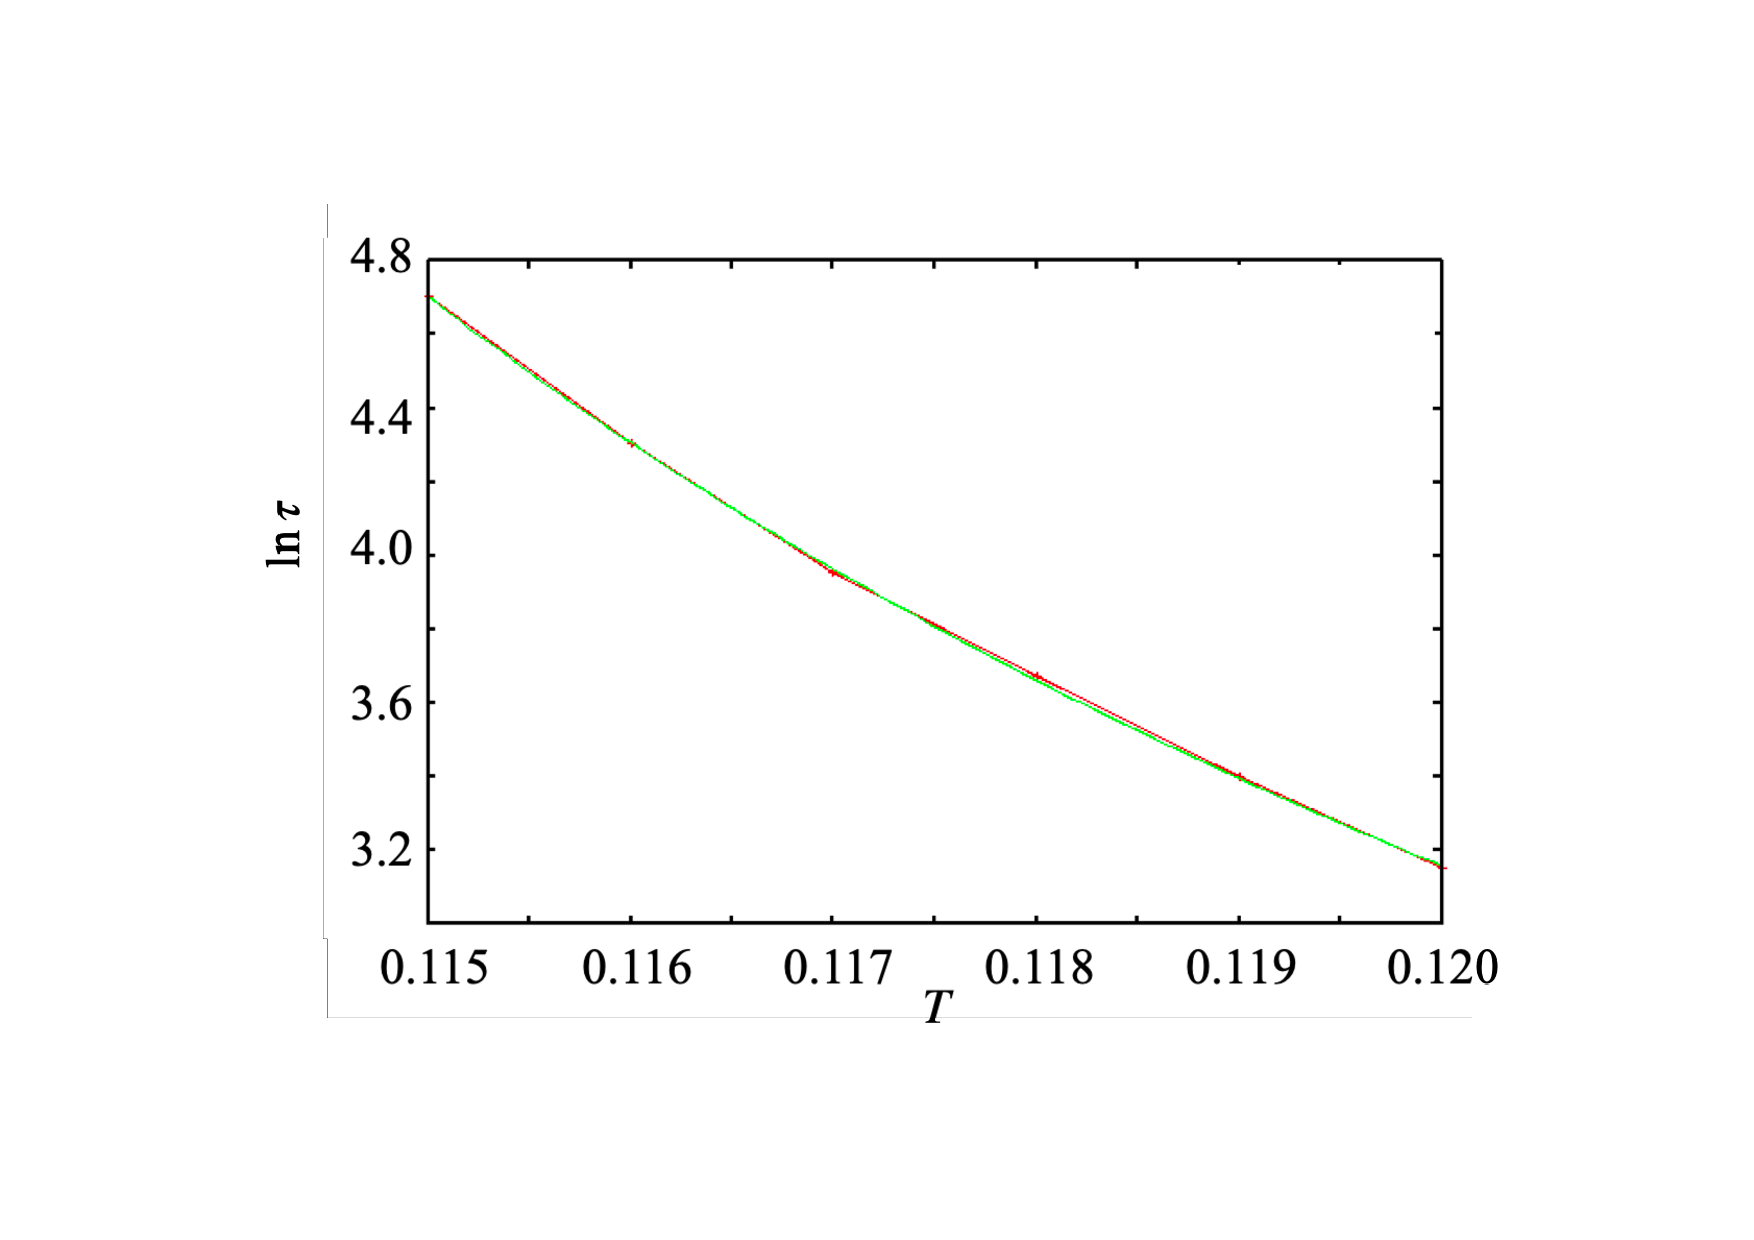
\includegraphics[width=12cm]{figure/mq_sqrt3_Tc_j2_0.02.pdf}
   \caption{$J_2=0.02$の$\sqrt{3}\times\sqrt{3}$磁気秩序変数の緩和時間の温度依存性}
\end{figure}

\begin{figure}[H]
   \centering
   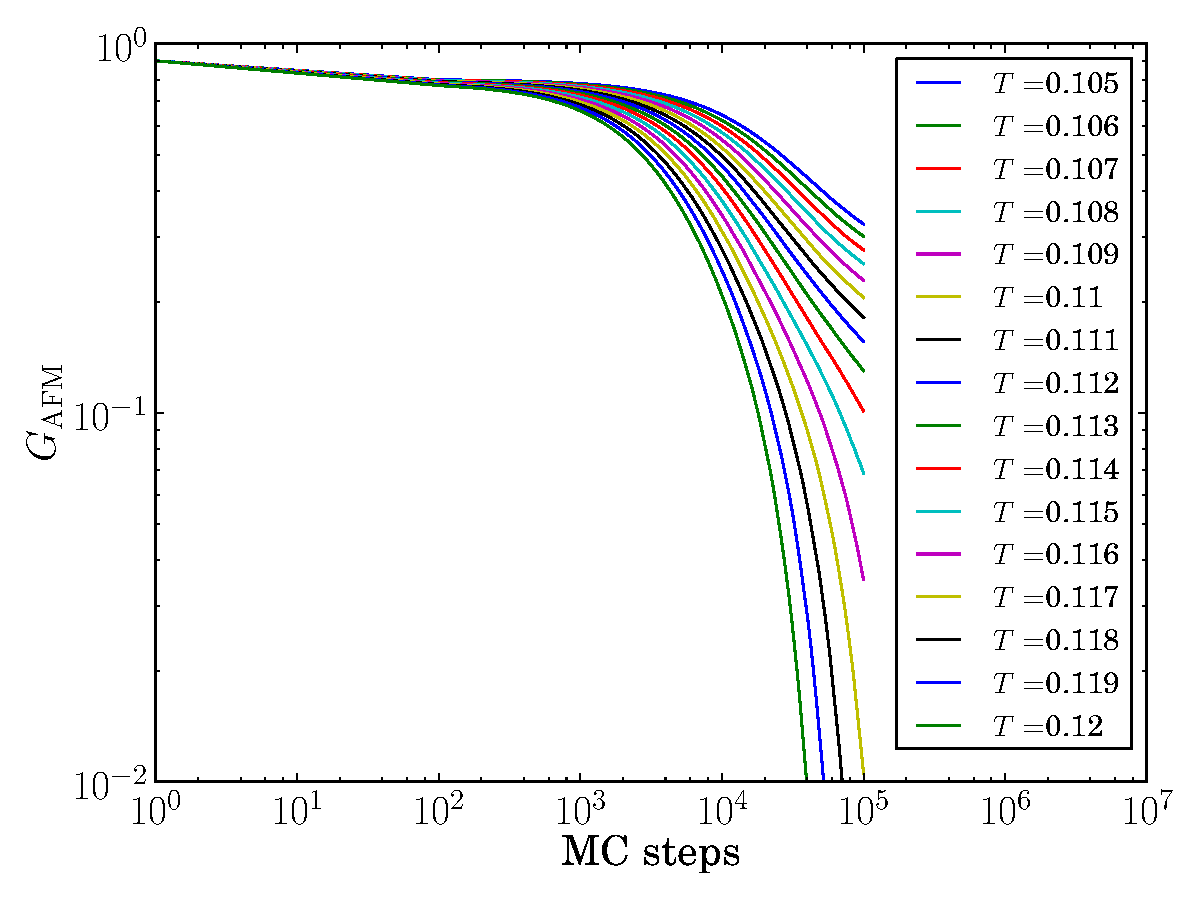
\includegraphics[width=12cm]{figure/afvc_raw_data_j2_0.02.pdf}
   \caption{$J_2=0.02$の反強磁性カイラリティ秩序変数の緩和過程}
\end{figure}

\begin{figure}[H]
   \centering
   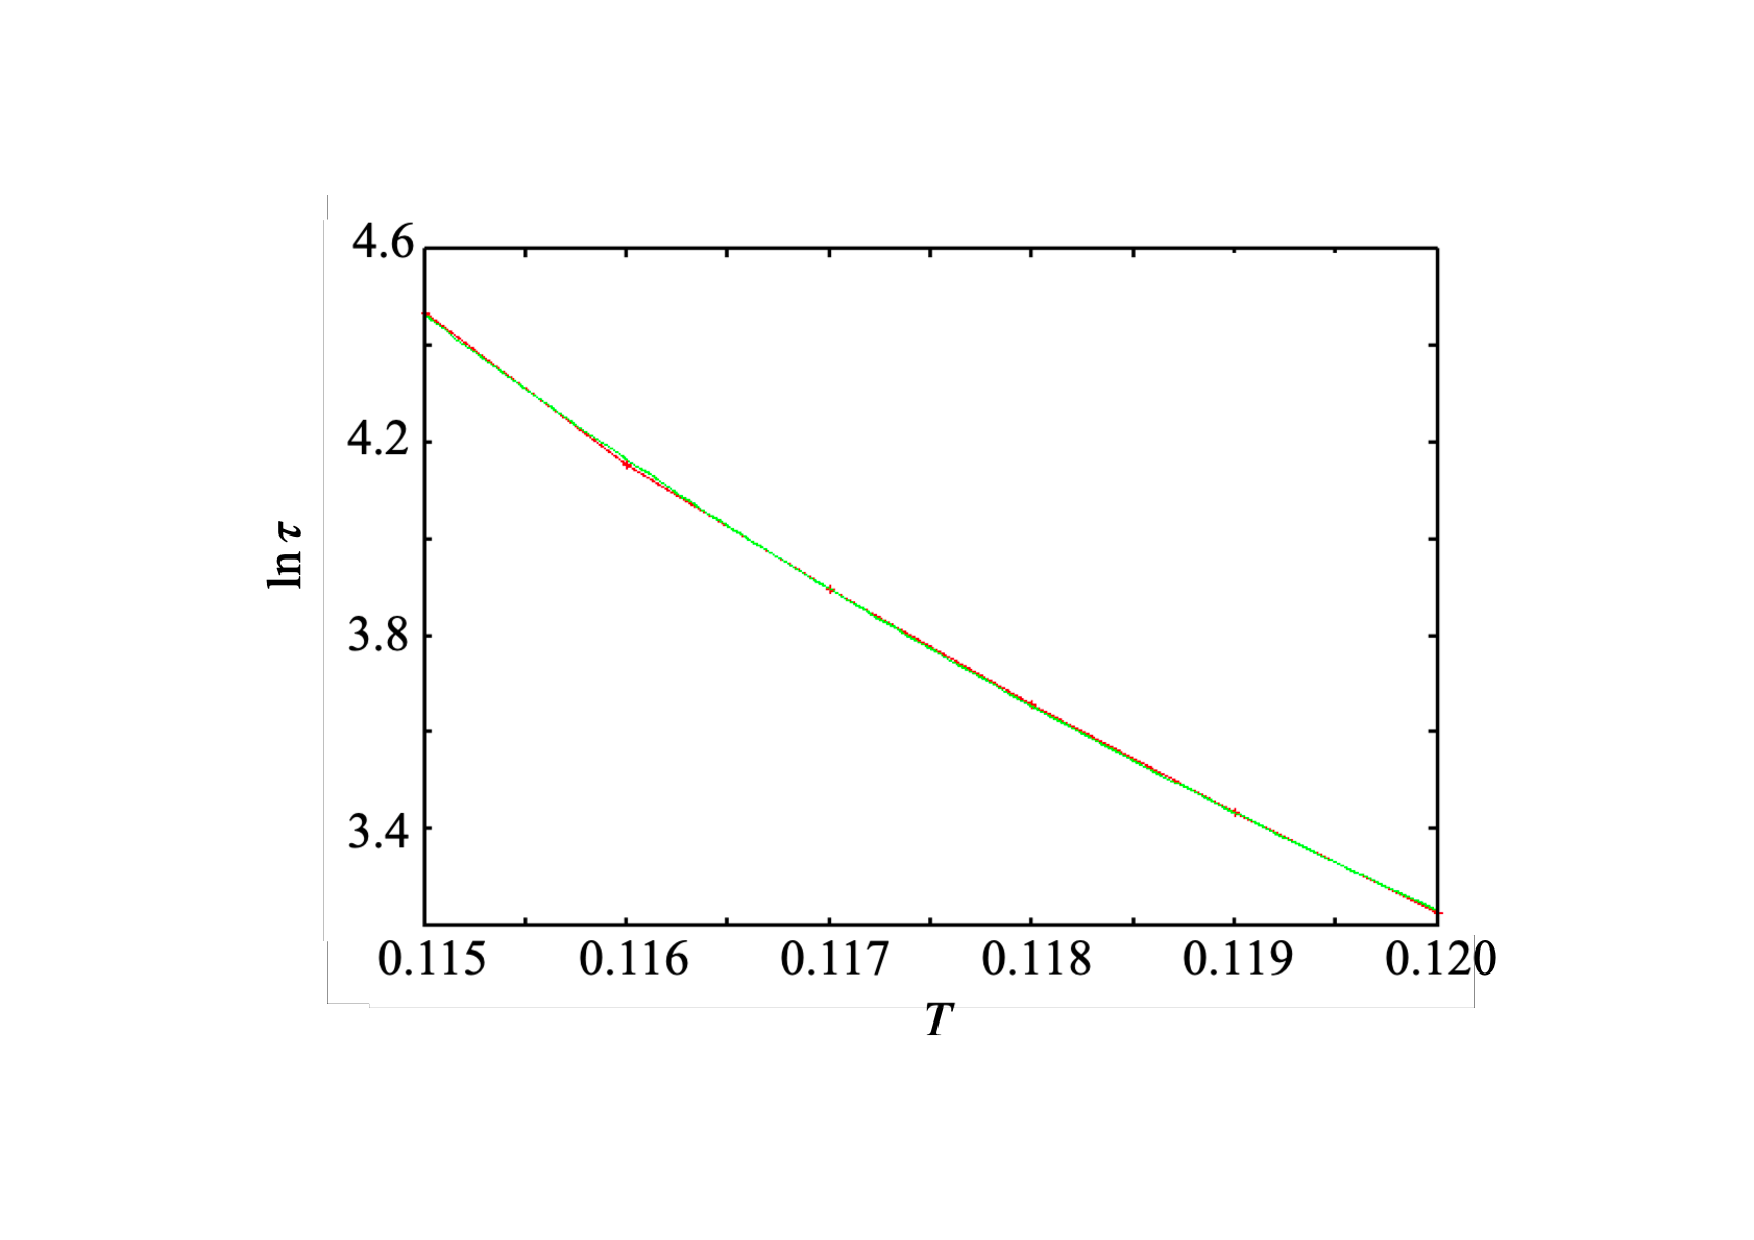
\includegraphics[width=12cm]{figure/afvc_Tc_j2_0.02.pdf}
   \caption{$J_2=0.02$の反強磁性カイラリティ秩序変数の緩和時間の温度依存性}
\end{figure}

\begin{figure}[H]
   \centering
   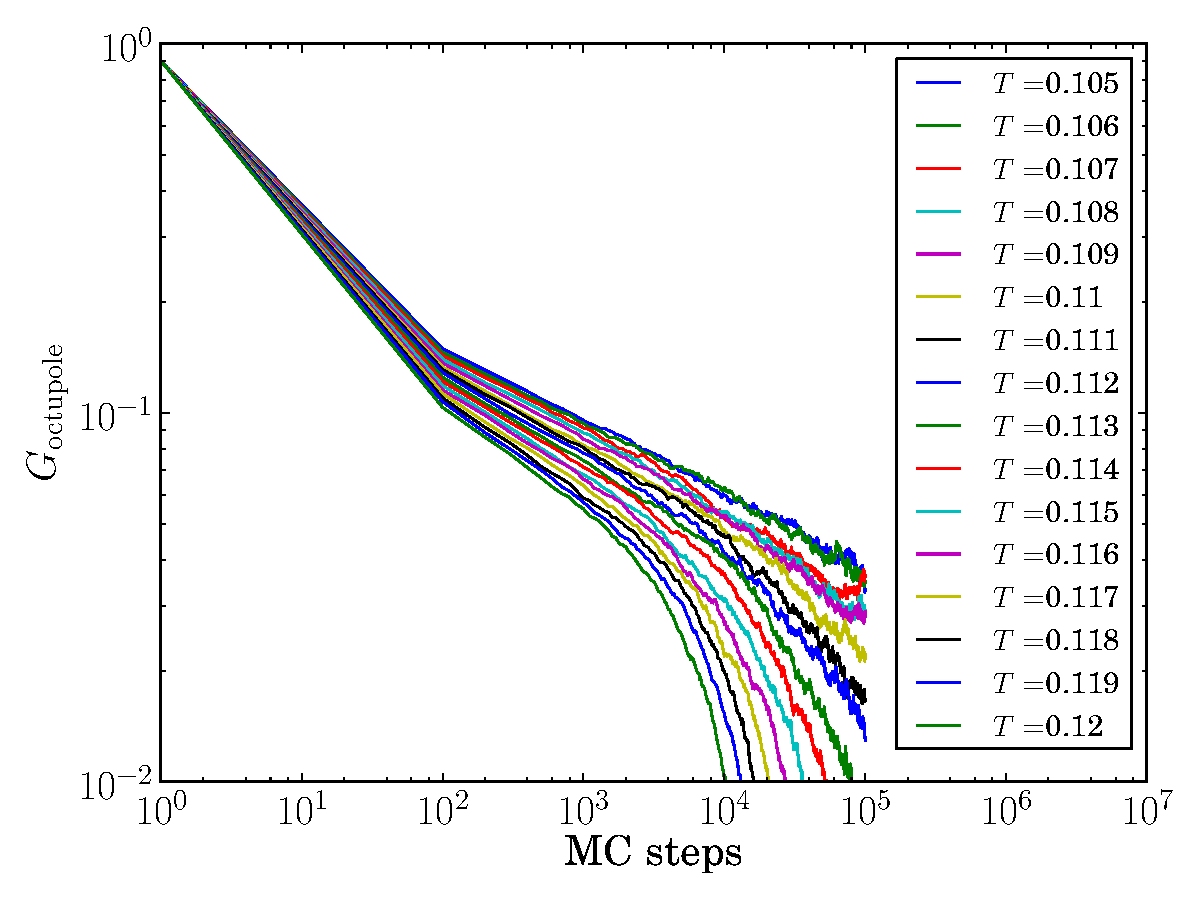
\includegraphics[width=12cm]{figure/octupole_raw_data_j2_0.02.pdf}
   \caption{$J_2=0.02$の八極子秩序変数の緩和過程}
\end{figure}

\begin{figure}[H]
   \centering
   \includegraphics[width=12cm]{figure/octupole_Tc_j2_0.02.pdf}
   \caption{$J_2=0.02$の八極子秩序変数の緩和時間の温度依存性}
\end{figure}


%\begin{figure}[H]
%   \centering
%   \includegraphics[width=15cm]{figure/relaxation_process_J2_0.01_2.pdf}
%   \caption{$J_2=0.01$のそれぞれの秩序変数の緩和過程と緩和時間の温度依存性}
%\end{figure}
%
%\begin{figure}[H]
%   \centering
%   \includegraphics[width=15cm]{figure/relaxation_process_J2_0.02_2.pdf}
%   \caption{$J_2=0.02$のそれぞれの秩序変数の緩和過程と緩和時間の温度依存性}
%\end{figure}

\newpage
\section{結論}
%本研究はカゴメ格子上の最近接古典反強磁性XY模型の基底状態の巨視的縮退に対する温度と次近接相互作用の協奏効果を数値的・定量的に解明することを目的に行われた。
本研究では大規模な古典モンテカルロ計算を行い、数値的な$J_2-T$相図を作成した。
まず、大域的な相構造は先行研究\cite{Korshunov2002}と整合するが、$-7\times10^{-2}\le J_2/J_1\le -7.5\times10^{-3}$に報告のない明確な一次転移が存在する。
%一次転移性は$J_2=-2\times10^{-2}$で最大となり、$J_2=-7\times10^{-2}$あるいは$J_2=-7.5\times10^{-3}$に近づくにつれ弱まる。
一次転移性は$J_2=-2\times10^{-2}$で最大となり、一次転移の終点に近づくにつれ弱まる。
また、$J_2<-7\times10^{-2}$でも有限サイズ効果によってエネルギーギャップが有限に残るため、高温側の終点を精密に決定することは難しい。
%一次転移領域の低温及び高温側の終点はエネルギーヒストグラムから推定できるが、精密な値を決定することは難しい。
次に、八極子相は$-5\times10^{-3}\le J_2/J_1\le2\times10^{-2}$に存在する。
%$J_2\le0$における八極子秩序に対する非平衡緩和法は$J_2=0,-2.5\times10^{-3}$で実行できたが、`'
また、非平衡緩和法の結果から、八極子秩序のBKT転移温度は$J_2$によって異なることがわかった。
さらに、一次転移の低温側の終点($J_2\sim-7.5\times10^{-3}$)は$q=0$相・八極子相・常磁性相の相境界($J_2\sim-5\times10^{-3}$)に近接している。
%これは低温での一次転移消失と八極子相の存在の間の関係を示唆している。
また、$J_2=0.02$において$2\times10^{-3}\si{\kelvin}$程度、反強磁性的カイラリティ転移と$\sqrt{3}\times\sqrt{3}$転移の転移温度が分離していることが確認できた。
これは長距離秩序であるカイラリティ秩序が準長距離秩序である$\sqrt{3}\times\sqrt{3}$秩序に比べ、温度ゆらぎに対してロバストであるという物理的直観に整合する。最後に、原点近傍の複雑な相構造は極低温における更新凍結によって確認されなかった。


%\newpage

\section{謝辞}
本修士論文を執筆する上で多くの方々に助言、協力をいただきました。特に学部四年と修士の二年の計三年の間、物理学の知識や数値計算、プログラミング技術について議論や質問に丁寧に対応して頂いた指導教員の品岡寛助教に感謝申し上げます。また、共同研究者であるBAQISの三澤貴宏さんにも協力、助言いただいたことに感謝申し上げます。また学内で日頃お世話になった物性理論研究室の星野晋太郎助教、学生の皆様にもこの場を借りて御礼申し上げます。最後に、親元を離れて大学に送り出してくれた家族に深く感謝を申し上げます。

\newpage

\bibliography{ref}
\bibliographystyle{junsrt}

\end{document}

\section{光電子分光}
物質の性質は主に電子が支配している。はじめに1電子近似において測定されるスペクトル関数について述べ、後半では電子相関がある多電子系で測定できるスペクトル関数について述べる\cite{pes}。

\subsection{1電子近似のスペクトル関数}

\begin{align}
   A(\omega) &= \frac{1}{\pi} \cdots\cdots\cdots\cdots\cdots\cdots\cdots\cdots\cdots\cdots
\end{align}
なお、複雑な数式を書くのは、physicsパッケージが便利らしい。

図をどう書くかは人の好みがあるが、ベクトル画像はPDF形式で保存して読み込むのがよい。
PNG形式でも良いが、拡大したときにぼやけたり、サイズが増える可能性がある。

Gnuplot, matplotlibを使う場合は、直接PDFファイル形式で保存可能。ベクトル形式のファイルを直接編集できるソフトとしては、Adobe/Illustrator, Inkscapeが有名。前者は高機能で値段分の価値はある。

\begin{figure}[ht]
  \centering
  \includegraphics[width=0.8\linewidth]{figure/zikken.png}
   \caption{角度光電子分光の概略図。横幅はincludegraphicsのオプションで調整可能。}
\end{figure}

\begin{figure}[ht]
  \centering
  \includegraphics[width=0.8\linewidth]{figure/bse3.pdf}
   \caption{PDFファイルも直接張り込めます。元ファイルはInkscapeで作ったfigure/bse3.svg}
\end{figure}

論文やHPのURLは、\begin{verbatim}\url \end{verbatim}コマンドを使う。

Google, \url{https://www.google.co.jp/}

大関真之. 「今日からできるスパースモデリング」\cite{sparse}。参考文献のbibtexにURLと閲覧日を記入する。

\section{手法}
\clearpage

\section{結果}
\clearpage

\section{まとめと今後の展望}
\clearpage

\section*{謝辞}
本修士論文を執筆する上で多くの方々に助言、協力をいただきました。特に$\cdots$

\bibliography{ref}
\bibliographystyle{junsrt}


\appendix
\section{手法の詳細}
